%% Copernicus Publications Manuscript Preparation Template for LaTeX Submissions
\documentclass[gmd, manuscript]{copernicus} %final manuscript
\definecolor{dark-gray}{gray}{0.55}

\begin{document}
\title{Emulating the GGCMI Phase II experiment: global gridded emulators of crop model responses to changes in CO2, temperature, nitrogen, and water (protocol version 1.0)}
%\title{GGCMI global gridded crop model emulators of yield and irrigation water demand}

\Author[1,2]{James}{Franke}
\Author[3]{Christoph}{M\"{u}ller}
\Author[2,4]{Joshua}{Elliott}
\Author[5]{Alex C.}{Ruane}
\Author[6]{Abigail}{Snyder}
\Author[3,2,4,5]{Jonas}{J\"{a}germeyr}
\Author[7,8]{Juraj}{Balkovic}
\Author[9,10]{Philippe}{Ciais}
\Author[11]{Marie}{Dury}
\Author[12]{Pete}{Falloon}
\Author[7]{Christian}{Folberth}
\Author[11]{Louis}{Fran{\c{c}}ois}
\Author[13]{Tobias}{Hank}
\Author[14,23]{Munir}{Hoffmann}
\Author[15,16]{R.\ Cesar}{Izaurralde}
\Author[11]{Ingrid}{Jacquemin}
\Author[15]{Curtis}{Jones}
\Author[7]{Nikolay}{Khabarov}
\Author[14]{Marian}{Koch}
\Author[2,17]{Michelle}{Li}
\Author[9,18]{Wenfeng}{Liu}
\Author[19]{Stefan}{Olin}
\Author[5,20]{Meridel}{Phillips}
\Author[21,22]{Thomas A.\ M.}{Pugh}
\Author[15]{Ashwan}{Reddy}
\Author[9,10]{Xuhui}{Wang}
\Author[12]{Karina}{Williams}
\Author[13]{Florian}{Zabel}
\Author[1,2]{Elisabeth}{Moyer}
%%%%%%%%%%%%%%%%%%%%%%%%%%%%%%
\affil[1]{Department of the Geophysical Sciences, University of Chicago, Chicago, IL, USA}
\affil[2]{Center for Robust Decision-making on Climate and Energy Policy (RDCEP), University of Chicago, Chicago, IL, USA}
\affil[3]{Potsdam Institute for Climate Impact Research, Member of the Leibniz Association, Potsdam, Germany}
\affil[3]{Department of Computer Science, University of Chicago, Chicago, IL, USA}
\affil[5]{NASA Goddard Institute for Space Studies, New York, NY, United States}
\affil[6]{Joint Global Change Research Institute, Pacific Northwest National Laboratory, College Park, MD, USA}
\affil[7]{Ecosystem Services and Management Program, International Institute for Applied Systems Analysis, Laxenburg, Austria}
\affil[8]{Department of Soil Science, Faculty of Natural Sciences, Comenius University in Bratislava, Bratislava, Slovak Republic}
\affil[9]{Laboratoire des Sciences du Climat et de l'Environnement, CEA-CNRS-UVSQ, 91191 Gif-sur-Yvette, France}
\affil[10]{Sino-French Institute of Earth System Sciences, College of Urban and Env. Sciences, Peking University, Beijing, China}
\affil[11]{Unit{\'{e}} de Mod{\'{e}}lisation du Climat et des Cycles Biog\'eochimiques, UR SPHERES, Institut d'Astrophysique et de G\'eophysique, University of Li\`ege, Belgium}
\affil[12]{Met Office Hadley Centre, Exeter, United Kingdom}
\affil[13]{Department of Geography, Ludwig-Maximilians-Universit\"{a}t, Munich, Germany}
\affil[14]{Georg-August-University G\"{o}ttingen, Tropical Plant Production and Agricultural Systems Modeling, G\"{o}ttingen, Germany}
\affil[15]{Department of Geographical Sciences, University of Maryland, College Park, MD, USA}
\affil[16]{Texas Agrilife Research and Extension, Texas A\&M University, Temple, TX, USA}
\affil[17]{Department of Statistics, University of Chicago, Chicago, IL, USA}
\affil[18]{EAWAG, Swiss Federal Institute of Aquatic Science and Technology, D\"{u}bendorf, Switzerland}
\affil[19]{Department of Physical Geography and Ecosystem Science, Lund University, Lund, Sweden}
\affil[20]{Earth Institute Center for Climate Systems Research, Columbia University, New York, NY, USA}
\affil[21]{School of Geography, Earth and Environmental Sciences, University of Birmingham, Birmingham, UK.}
\affil[22]{Birmingham Institute of Forest Research, University of Birmingham, Birmingham, UK.}
\affil[23]{Leibniz Centre for Agricultural Landscape Research (ZALF), D-15374 Müncheberg, Germany}
%%%%%%%%%%%%%%%%%%%%%%%%%%%%%%
\runningtitle{The GGCMI crop model emulators}
\runningauthor{Franke et al.}
\correspondence{James Franke (jfranke@uchicago.edu)}
%%%%%%%%%%%%%%%%%%%%%%%%%%%%%%

%% These dates will be inserted by Copernicus Publications during the typesetting process.
\received{}
\pubdiscuss{} %% only important for two-stage journals
\revised{}
\accepted{}
\published{}
%%%%%%%%%%%%%%%%%%%%%%%%%%%%%%
\firstpage{1}
\maketitle
%%%%%%%%%%%%%%%%%%%%%%%%%%%%%%
\begin{abstract}
\textcolor{red}{
Statistical emulation of process-based crop models provides the opportunity to combine some of the advantageous features of statistical and process-based crop models.  
The Global Gridded Model Intercomparison Project (GGCMI) Phase II consists of a set of simulations run on a suit of process based models with an explicit goal of producing a structured training dataset for crop model emulator development.
In this study we present the construction of a set of crop model emulators of mean-climatological yield for nine process-based crop models and five crops.
The GGCMI Phase II systematic parameter sweep protocol allows disentangling the climate-driven mean response from year-over-year variations; we show that the two responses have very different relationships to standard climate metrics such as mean growing season temperature. 
The climatological mean yield response can be readily represented with a simple polynomial in almost all locations where crops are currently grown, permitting a tool that captures model responses in a lightweight, computationally tractable form. 
Crop model emulation should therefore facilitate both model comparison and integrated assessment of climate impacts.
}
\end{abstract}

%\copyrightstatement{TEXT}

\introduction
\label{S:1}
Improving our understanding of the impacts of future climate change on crop yields is critical for global food security in the twenty-first century. 
Projections of future yields under climate change are generally made with one of two approaches: either process-based models, which  simulate the process of photosynthesis and the biology and phenology of individual crops, or statistical models, which use historical weather and yield data to capture relationships between observed crop yields and major drivers.
Process-based crop models provide some advantages, including capturing the direct effects of CO$_2$ fertilization and allowing projections in areas where crops are not currently grown. 
%including providing a clear mechanism for linking climate to yield outcomes.
However, they are computationally expensive, and can be difficult or impossible to directly integrate into larger climate change impacts assessments.
Statistical crop models can only capture crop responses under the range of current conditions, but have several advantages: they implicitly include management and behavioral practices that are difficult to model explicitly, and they are typically simple analytical expressions that are easily implemented by downstream impact modelers. 
Both types of models are routinely used, and comparative studies have concluded that when done carefully, both approaches can provide similar yield estimates \citep[e.g.][]{Lobell2010, Moore2017, Roberts2017, zhao2017}. 

Statistical emulation allows combining some of the advantageous features of both statistical and process-based models.
Crop model emulators allow representing process-based crop model responses in a computationally-inexpensive form appropriate for economic assessments, and assist in crop model intercomparison and improvement efforts.
The approach involves constructing a ``surrogate model'' of numerical simulations by using their output as training data for a statistical representation \citep[e.g.][]{OHAGAN2006, OHAGAN2010}. 
Emulation is particularly useful in cases where simulations are complex and output data volumes are large, and has been used in a variety of fields, including hydrology \citep[e.g.][]{Razavi2012}, engineering \citep[e.g.][]{STORLIE2009}, environmental sciences \citep[e.g.][]{RATTO2012}, and climate \citep[e.g.][]{Castruccio14, Holden2014}. 
For agricultural impacts studies, emulation of process-based models allows capturing key relationships between input variables in a lightweight, flexible form that is compatible with economic studies. Emulation allows producing yield projections under arbitrary emissions scenarios and is an important diagnostic tool for model comparison and model evaluation.

Interest is rising in applying statistical emulation to crop models, and multiple studies have developed crop model emulators in the past decade.
Early studies proposing or describing potential crop yield emulators include \citet{Howden2005, raisen2006, Lobell2010}, and \citet{Ferrise2011}, who used a machine learning approach to predict Mediterranean wheat yields. 
Studies developing single-model emulators include  \citet{Holzkamper2012} for the CropSyst model, \citet{RUANE2013a} for the CERES wheat model, and \citet{Oyebamiji15} for the LPJmL model. 
More recently, emulators have begun to be used in the context of multi-model intercomparisons, with multiple authors \citep{BLANC2015, BLANC2017, Ostberg2018, Mistry2017}  using them to analyze the five crop models  of the Inter-Sectoral Impacts Model Intercomparison Project (ISIMIP). ISIMIP offers a relatively large traning set --  control, historical, and several Representative Concentration Pathway (RCP) scenarios using output from up to five climate models \citep{Warszawski3228, Frieler2017} -- and choices of emulation strategy differ.
\citet{BLANC2015} and \citet{BLANC2017} use historical and RPC8.5 scenarios, combine multiple climate model projections for RCP8.5, and regress across soil regions. 
%\textcolor{red}{don't understand: and use local weather variables and yields in their regress across soil regions}. 
\citet{Ostberg2018} use global mean temperature change (and CO$_2$) as regressors, and then pattern-scales to emulate local yields. 
\citet{Mistry2017} compare emulated and observed historical yields, using local weather data and a historical crop simulation. 
The constraints of the ISIMIP experiment mean that all these efforts do share important common features. 
All emulate annual crop yields along an entire scenario or scenarios, and all future climate scenarios are non-stationary, with important covariates (temperature and precipitation for example) evolving simultaneously. % which may make diagnosing the individual and interacting affects difficult.  

An alternative approach to emulation involves construction of a ``parameter sweep'' training set, a collection of multiple stationary scenarios that systematically cover a range of input parameter values.
A parameter sweep offers several important advantages for emulation over an experiment in which climate evolves over time. 
First, it allows separating the effects of different variables that affect yields but that are highly correlated in realistic future scenarios (e.g.\ CO$_2$ and temperature). 
such as those of ISIMIP.
Second, it allows making a distinction between year-over-year yield variations and climatological changes, which may involve different responses to the particular climate regressors used \citep[e.g.][]{Ruane2016}. 
For example, if year-over-year yield variations are driven predominantly by variations in the distribution of temperatures throughout the growing period, and long-term climate changes are driven predominantly by shifts in means, then regressing on the mean growing period temperature will produce different yield responses at annual vs.\ climatological timescales.  

Systematic parameter sweeps have begun to be used in crop model evaluation and emulation, with early efforts in 2014 and 2015 \citep{ruane2014, Markowski2015, Pirttioja2015}, and several recent studies in 2018 \citep{FRONZEK20182, Snyder2018, RUIZRAMOS2018}. 
All three 2018 studies sample multiple perturbations to temperature and precipitation, and two of the three add CO$_2$ as well, for a total of 132, 99 and 220 different combinations, respectively. 
All take advantage of the structured training set to construct emulators (``response surfaces'') of climatological mean yields, omitting year-over-year variations. 
All studies have some limitations, however, for assessing global agricultural impacts. None offer global coverage, but instead focus on a limited number of sites. Two involve many crop models but only one crop (wheat) \citep{FRONZEK20182,RUIZRAMOS2018}, while \citet{Snyder2018} analyzes four crops (maize, wheat, rice, soy) but only in one crop model (GCAM) \citep{calvin2019}.

In this paper we describe a set of globally-gridded crop model emulators developed from the new parameter-sweep dataset of the Global Gridded Crop Model Intercomparison (GGCMI) Phase II effort. 
GGCMI Phase II, a part of the Agricultural Model Intercomparison and Improvement Project (AgMIP) \citep{ROSENZWEIG2013, Rosenzweig2014}, provides the first near-global-coverage systematic parameter sweep of multi-model crop simulations, and is specifically designed for construction of agricultural emulators,  
%\textcolor{red}{The experiment involves twelve different globally gridded crop models, each simulating multiple crops (maize, rice, soy and spring and winter wheat) over as many as 1400 simulations, each driven by historical climate inputs with systematically perturbations to CO$_2$, temperature, precipitation, and nitrogen application (CTWN).
%The resulting dataset allows }
to allow diagnosing the effects on crop yields of both individual factors and their joint effects.
In the following, we describe the training dataset (Section \ref{S:2}), the statistical model used for emulation (Section \ref{S:3}), measures of emulator fidelity (Section \ref{S:4}), and examples of preliminary results (Section \ref{S:5}). 

%is the most comprehensive crop model emulation effort to date, significantly expanding the scope of previous parameter-sweep crop model emulation work by incorporating 

%%%%%%%%%%%%%%%%%%%%%%%%%%%%%%%%%%%%%%%%%%%%%%%%%%%%%%%%%%%%%%%
%%%%%%%%%%%%%%%%%%%%%%%%%%%%%%%%%%%%%%%%%%%%%%%%%%%%%%%%%%%%%%%
%%%%%%%%%%%%%%%%%%%%%%%%%%%%%%%%%%%%%%%%%%%%%%%%%%%%%%%%%%%%%%%
\section{Training dataset}
\label{S:2}
\subsection{The GGCMI Phase II dataset}
\begin{table*}[t]
\caption{
Crop models included in GGCMI Phase II emulators and the number of CTWN-A simulations performed for each model. 
The maximum number is 756 for A0 (no adaptation) experiments, and 648 for A1 (maintaining growing length) experiments, since T0 is not simulated under A1. ``N-Dim.'' indicates whether the models are able to represent varying nitrogen levels.
Each model provides the same set of CTWN simulations across all its modeled crops, but some models omit individual crops. 
(For example, CARAIB does not simulate spring wheat.)
Table adapted from \citet{Franke2019a}. 
The three simulation models not included in the emulators have been removed for clarity.
}
\label{table:models}
  \begin{tabular}{p{6cm} p{1cm} p{1cm} p{1cm} p{1cm} p{1cm} p{1cm} p{1.9cm}}
    \tophline
    {\textbf{Model (Key Citations)}}&{\textbf{Maize}}&{\textbf{Soybean}}&{\textbf{Rice}}&{\textbf{Winter wheat}}&{\textbf{Spring wheat}}&{\textbf{N dim.}}&{\textbf{Sims per crop (A0 / A1)}}\\ \middlehline
    {\textbf{CARAIB},    \citet{Dury2011, Pirttioja2015}}  & {X} & {X} & {X} & {X} & {X} & {--} & {\textbf{252 / 216}}\\ \middlehline
    {\textbf{EPIC-TAMU}, \citet{Izaurralde06}} & {X} & {X} & {X} & {X} & {X} & {X} & {\textbf{756 / 648}}\\ \middlehline
    {\textbf{JULES},     \citet{Osborne2015, Williams2015, Williams2017}} & {X} & {X} & {X} & {--} & {X} & {--} & {\textbf{252 / 0}}\\ \middlehline
    {\textbf{GEPIC},     \citet{LIU2007478, FOLBERTH201221}} & {X} & {X} & {X} & {X} & {X} & {X} & {430 / 181}\\ \middlehline
    {\textbf{LPJ-GUESS}, \citet{Lindeskog2013, Olin2015}} & {X} & {--} & {--} & {X} & {X} & {X} & {\textbf{756 / 648}}\\  \middlehline
    {\textbf{LPJmL},     \citet{von_Bloh_implementing_2018}} & {X} & {X} & {X} & {X} & {X} & {X} & {\textbf{756 / 648}}\\ \middlehline
    {\textbf{pDSSAT},    \citet{Elliott2014b, JONES2003235}} & {X} & {X} & {X} & {X} & {X} & {X} & {\textbf{756 / 648}}\\ \middlehline
    {\textbf{PEPIC},     \citet{LIU2016164, LIU2016}}  & {X} & {X} & {X} & {X} & {X} & {X} & {149 / 121}\\ \middlehline
    {\textbf{PROMET},    \citet{Hank2015, MAUSER2015}} & {X} & {X} & {X} & {X} & {X} & {X} & {261 / 232}\\
    \bottomhline
  \end{tabular}
\end{table*}

\begin{table}[t]
\caption{GGCMI Phase II input levels for the parameter sweep. 
Temperature and precipitation values are the perturbations from the historical climatology. 
W-percentage does not apply to the irrigated (W$_{inf}$) simulations, which are all simulated at the maximum beneficial levels of water. 
Bold font indicates the `baseline' historical level. One model provided simulations at the T + 5 level. 
See Figure SX in the supplement for number of simulations associated with each combination of input levels.
Table repeated from \citet{Franke2019a} 
%The GGCMI Phase II simulation model inputs are harmonized wherever possible including planting days (which vary spatially) and growing season lengths.
}
\label{table:inputs} 
    \begin{tabular}{lcc} 
        \tophline \vspace{1mm}
        \textbf{Input variable} & \textbf{Tested range} & \textbf{Unit} \\ \middlehline \vspace{1mm}
        [CO$_2$] (C) & \textbf{360}, 510, 660, 810 & ppm\\ \middlehline \vspace{1mm}
        Temperature (T) & -1, \textbf{0}, 1, 2, 3, 4, 6 & $^{\circ}$C\\ \middlehline \vspace{1mm}
        Precipitation (W) & -50, -30, -20, -10, \textbf{0}, & \% \\
        {} & 10, 20, 30, (and W$_{inf}$) & {} \\ \middlehline \vspace{1mm}
        Applied nitrogen (N) & 10, 60, \textbf{200} & kg ha$^{-1}$ \\ \middlehline \vspace{1mm}
        Adaptation (A) & \textbf{A0: none}, A1: new cultivar to maintain original growing season length & -\\ \bottomhline
    \end{tabular}\\
\end{table}

The GGCMI Phase II simulations are described in detail in \citet{Franke2019a}, but we summarize briefly here. 
The experiment involves nine different globally gridded crop models, each simulating multiple crops (maize, rice, soy, and spring and winter wheat) across a parameter sweep of as many as 1400 scenarios, each driven by a historical climate timeseries with systematic perturbations to CO$_2$, temperature, precipitation, and nitrogen application (CTWN). 
%The resulting dataset allows diagnosing effects on crop yields of both the individual factors and their joint effects.}
Table \ref{table:models} shows the participating models and the scenarios that each provides, and Table \ref{table:inputs} shows the specified 4 levels of atmospheric CO$_2$, 7 of temperature, 8 of precipitation, and 3 of applied nitrogen. 
These simulations are repeated four times, for irrigated and rainfed crops, and for fixed growing seasons and growing seasons lengthening in warmer climates. 
(Fixed and lengthening growing-season scenarios are termed A0 and A1, respectively.) 
The complete protocol for a modeling group involves up to 19,440 years of global simulated output for rainfed crop and growing-season case; or 42,120 years across all simulations for a single modeling group. 
Because the computational demand is high, modeling groups were allowed to submit at various specified levels of participation, with the lowest level of participation consisting of 20\% of the maximum possible simulations; the mean participation level is 65\% of max potential runs.

Each individual crop model simulation is run for 30 years over historic weather for the period of 1981-2010, with added uniform perturbations to any of the CTWN variables.
Historical weather is taken for most models from the AgMERRA \citep{Ruane2015} historical daily climate data product, but the PROMET model uses the ERA-Interim reanalysis \citep{dee2011era} and the JULES model uses a bias-corrected version of ERA-Interim, WFDEI (WATCH-Forcing-Data-ERA-Interim) \citep{weedon2014wfdei}. 
Temperature perturbations are applied as additive mean shifts (from -1 to +6 degrees C), precipitation as fractional multipliers (from -50\% to +30\%), and CO$_2$ and nitrogen application as fixed values. (See Table \ref{table:inputs} for all values.)
Models provide global output at 0.5 degree latitude and longitude resolution for each simulation year.

%Some models share a common genealogy, but have since branched and developed independently, and will be treated independently in this work. 
%Minor differences in historical rainfall across the different reanalysis products used result in differences in the precipitation shift in the parameter-sweep. 
%Atmospheric CO$_2$ and applied nitrogen fertilizer take uniform, static values globally for each 30-year simulation case.
%Sampling across the parameter sweep is heterogeneous across models so the resultant training dataset size differs across models. 
%(See Table \ref{table:models} for number of 30-year simulations).

%%%%%%%%%%%%%%%%%%%%%%%%%%%%%%%%%%%%%%%%%%%%%%%%%%%%
\subsection{Climatological vs. year-to-year response}
\begin{figure}[ht]
\centering
   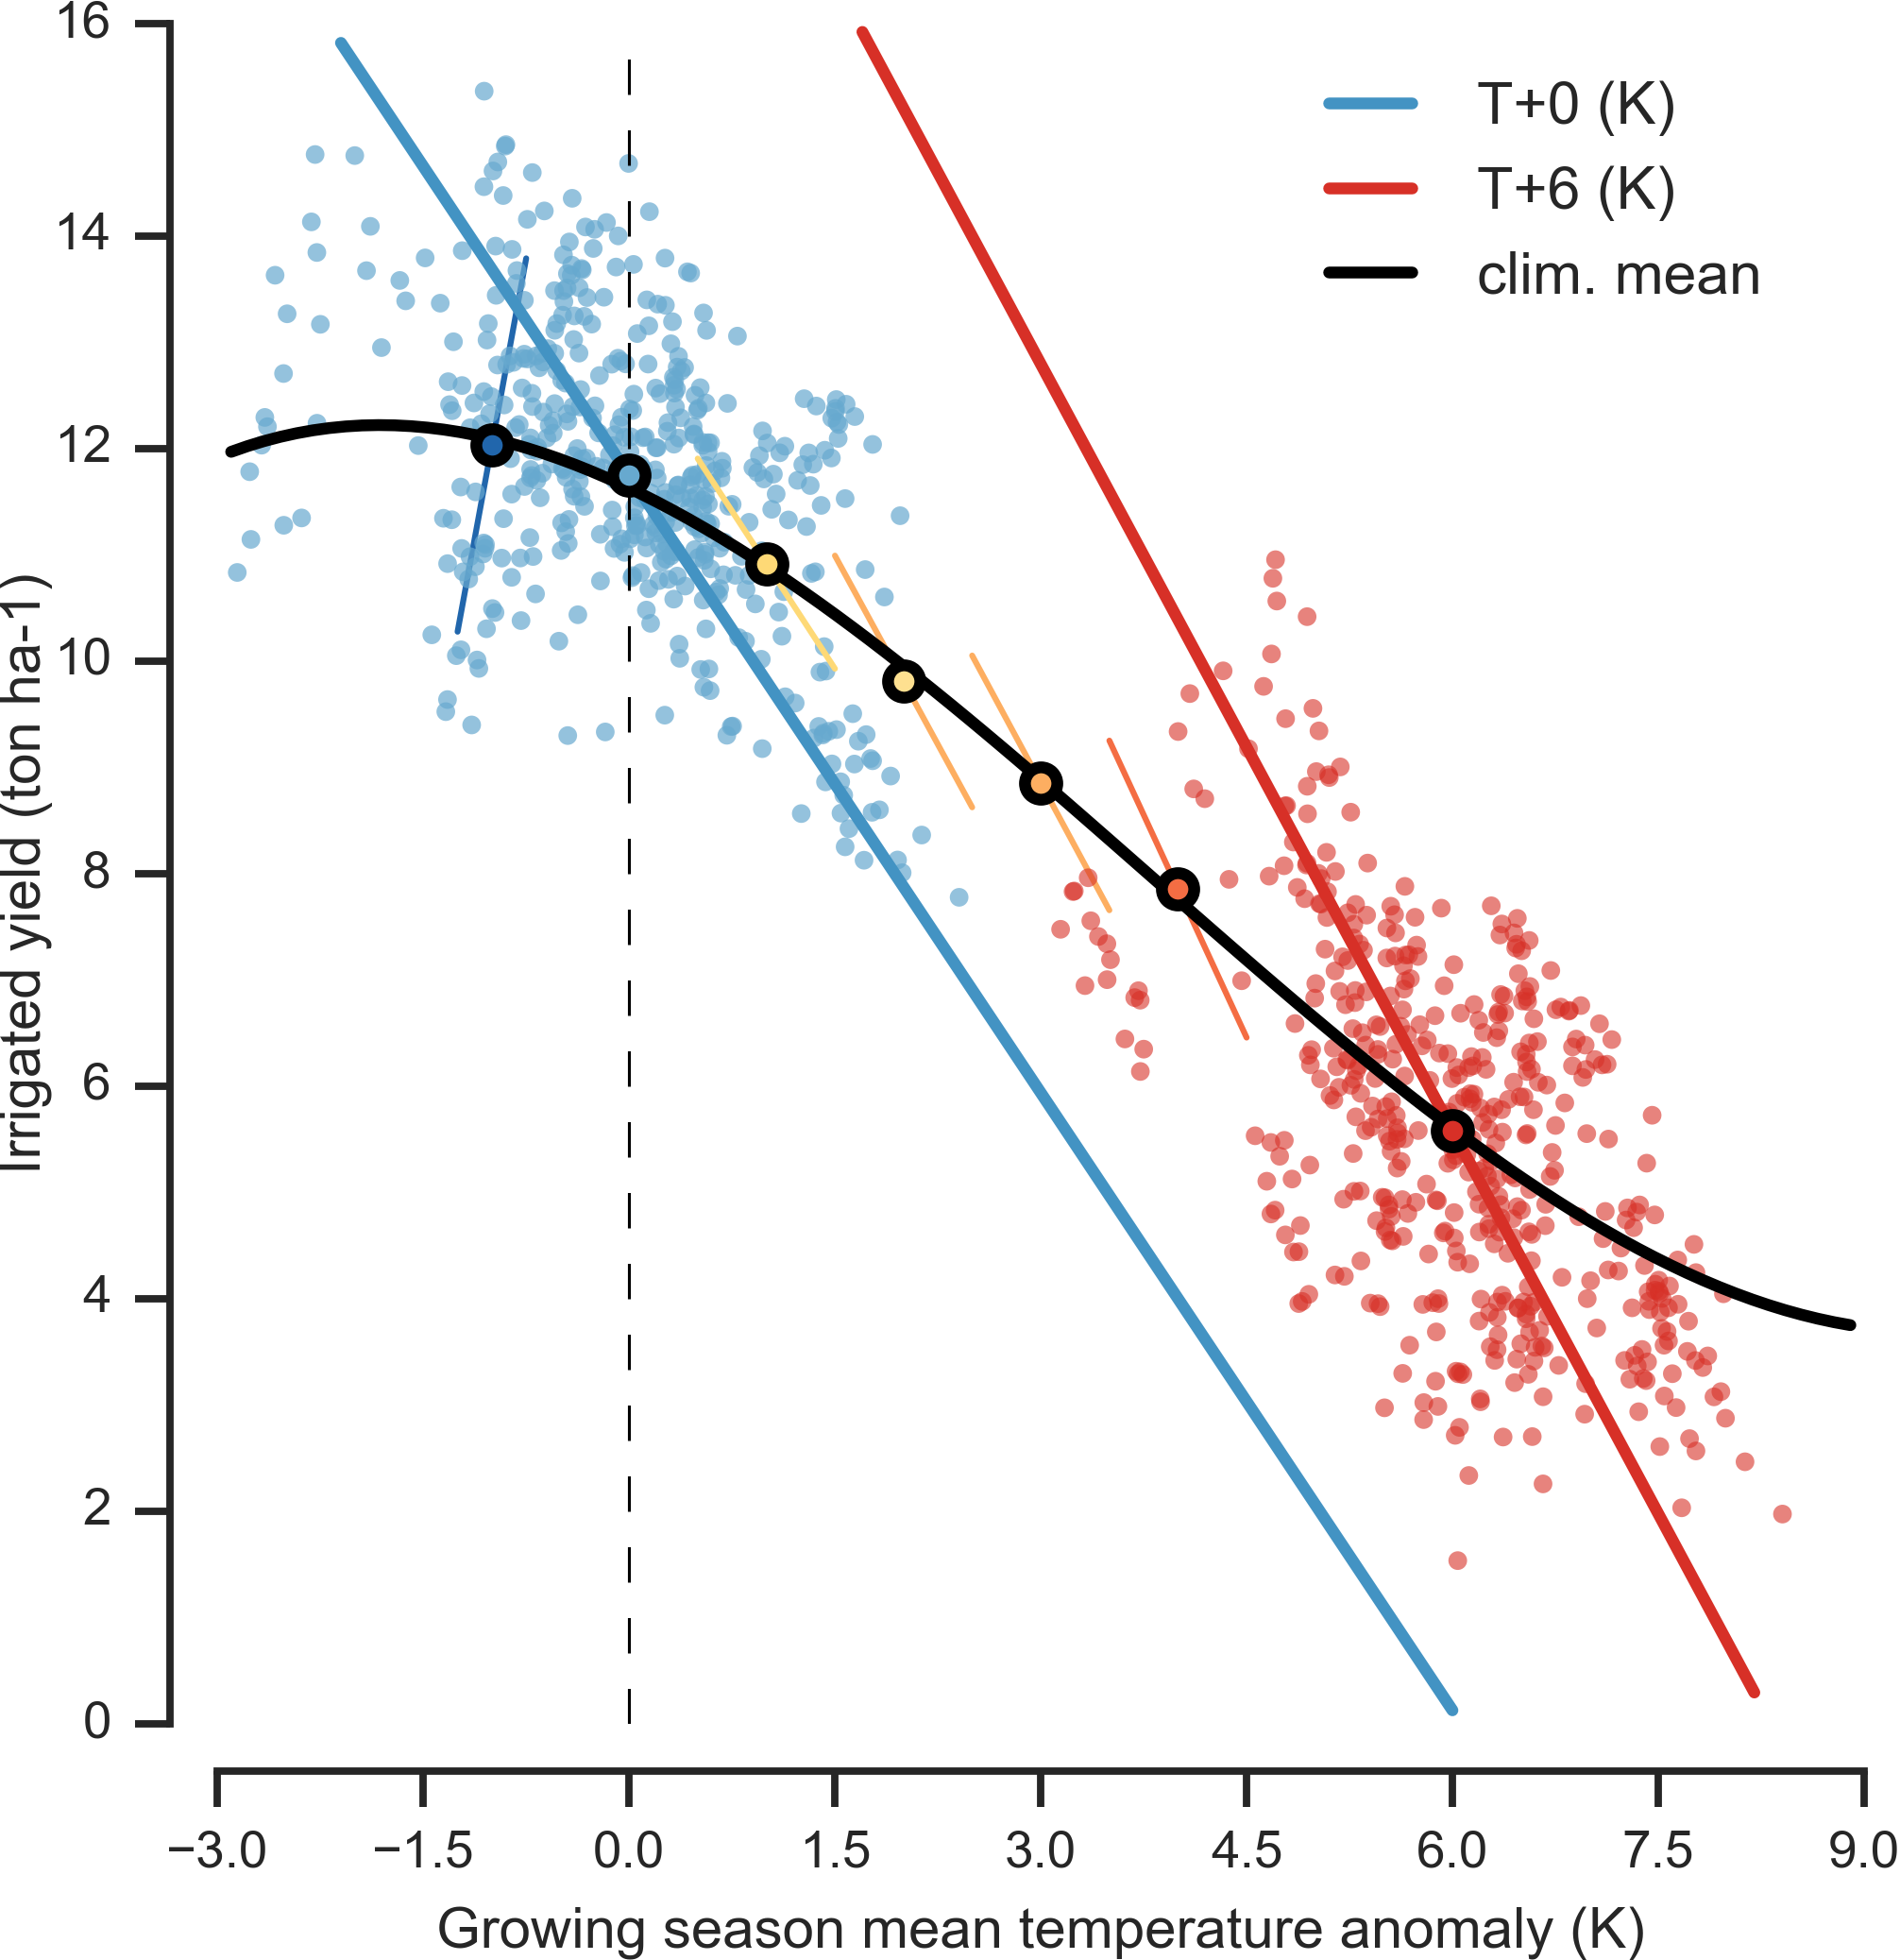
\includegraphics[width=7cm]{figures/tempyearvclim.png} \hspace{10mm} 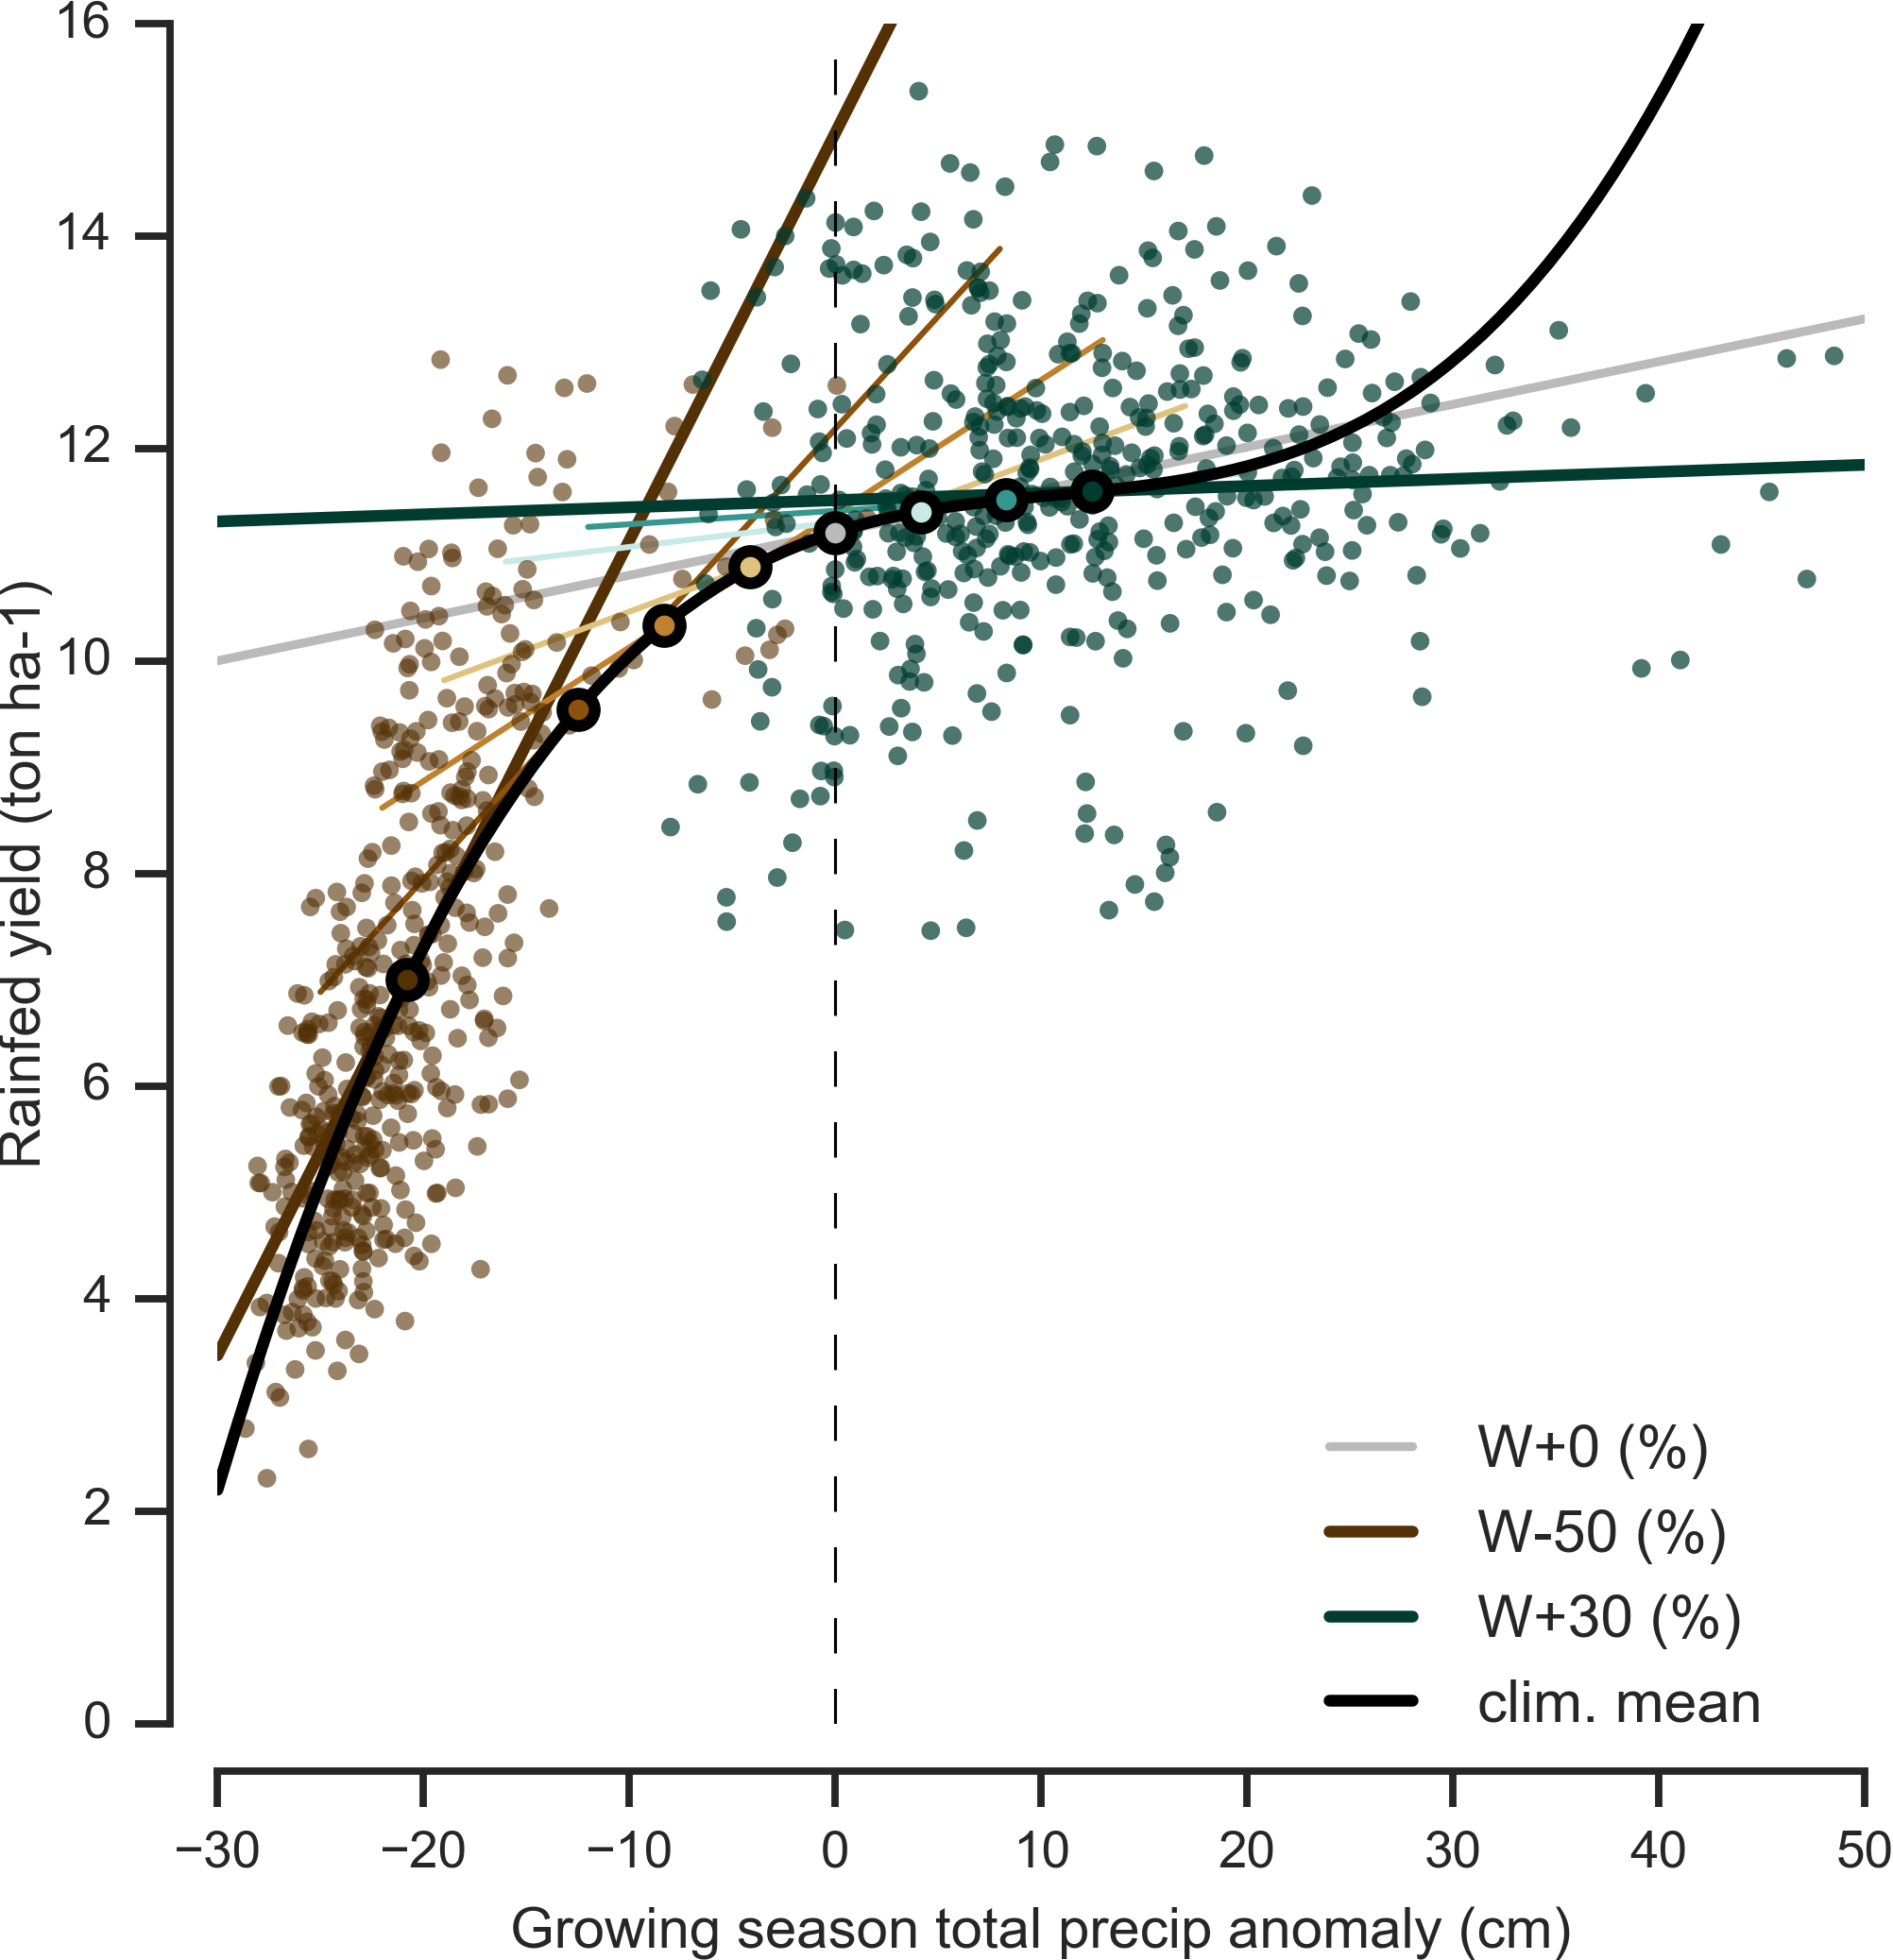
\includegraphics[width=7cm]{figures/pryearvclim.png}
   \caption{
   Example showing distinction between crop yield responses to year-to-year and climatological mean temperature and precipitation shifts. Figures shows
	maize for a representative high-yield region (nine adjacent grid cells in northern Iowa) from the pDSSAT model \textit{Left}: irrigated maize, climatological mean values for all temperature cases (T-1, +0, +1, +2, +3, +4, +6) with other variables held at baseline values, and individual years for T+0, blue, and T+6 K, red. \textit{Right}: rainfed maize, all precipitation cases (W -50\%, -30\%, -20\%, -10\%, W, +10\%, +20\%, +30\%), with individual years shown for W-50\%, grown, and W+50\%, green.
	Open black circles mark climatological mean yields for each case and short colored lines the linear regression to individual yields in each case. Bold black lines show 3rd order polynomial fits through climatological mean values. 
   In the temperature case, year-over-year yield responses are very different from the response to longer-term climate perturbations, and rise under warmer conditions. In the precipitation case, year-over-year responses resemble the climatological mean response, but the response is highly nonlinear.}
   \label{fig:yearvclim}
\end{figure}

\begin{figure}[ht]
\centering
   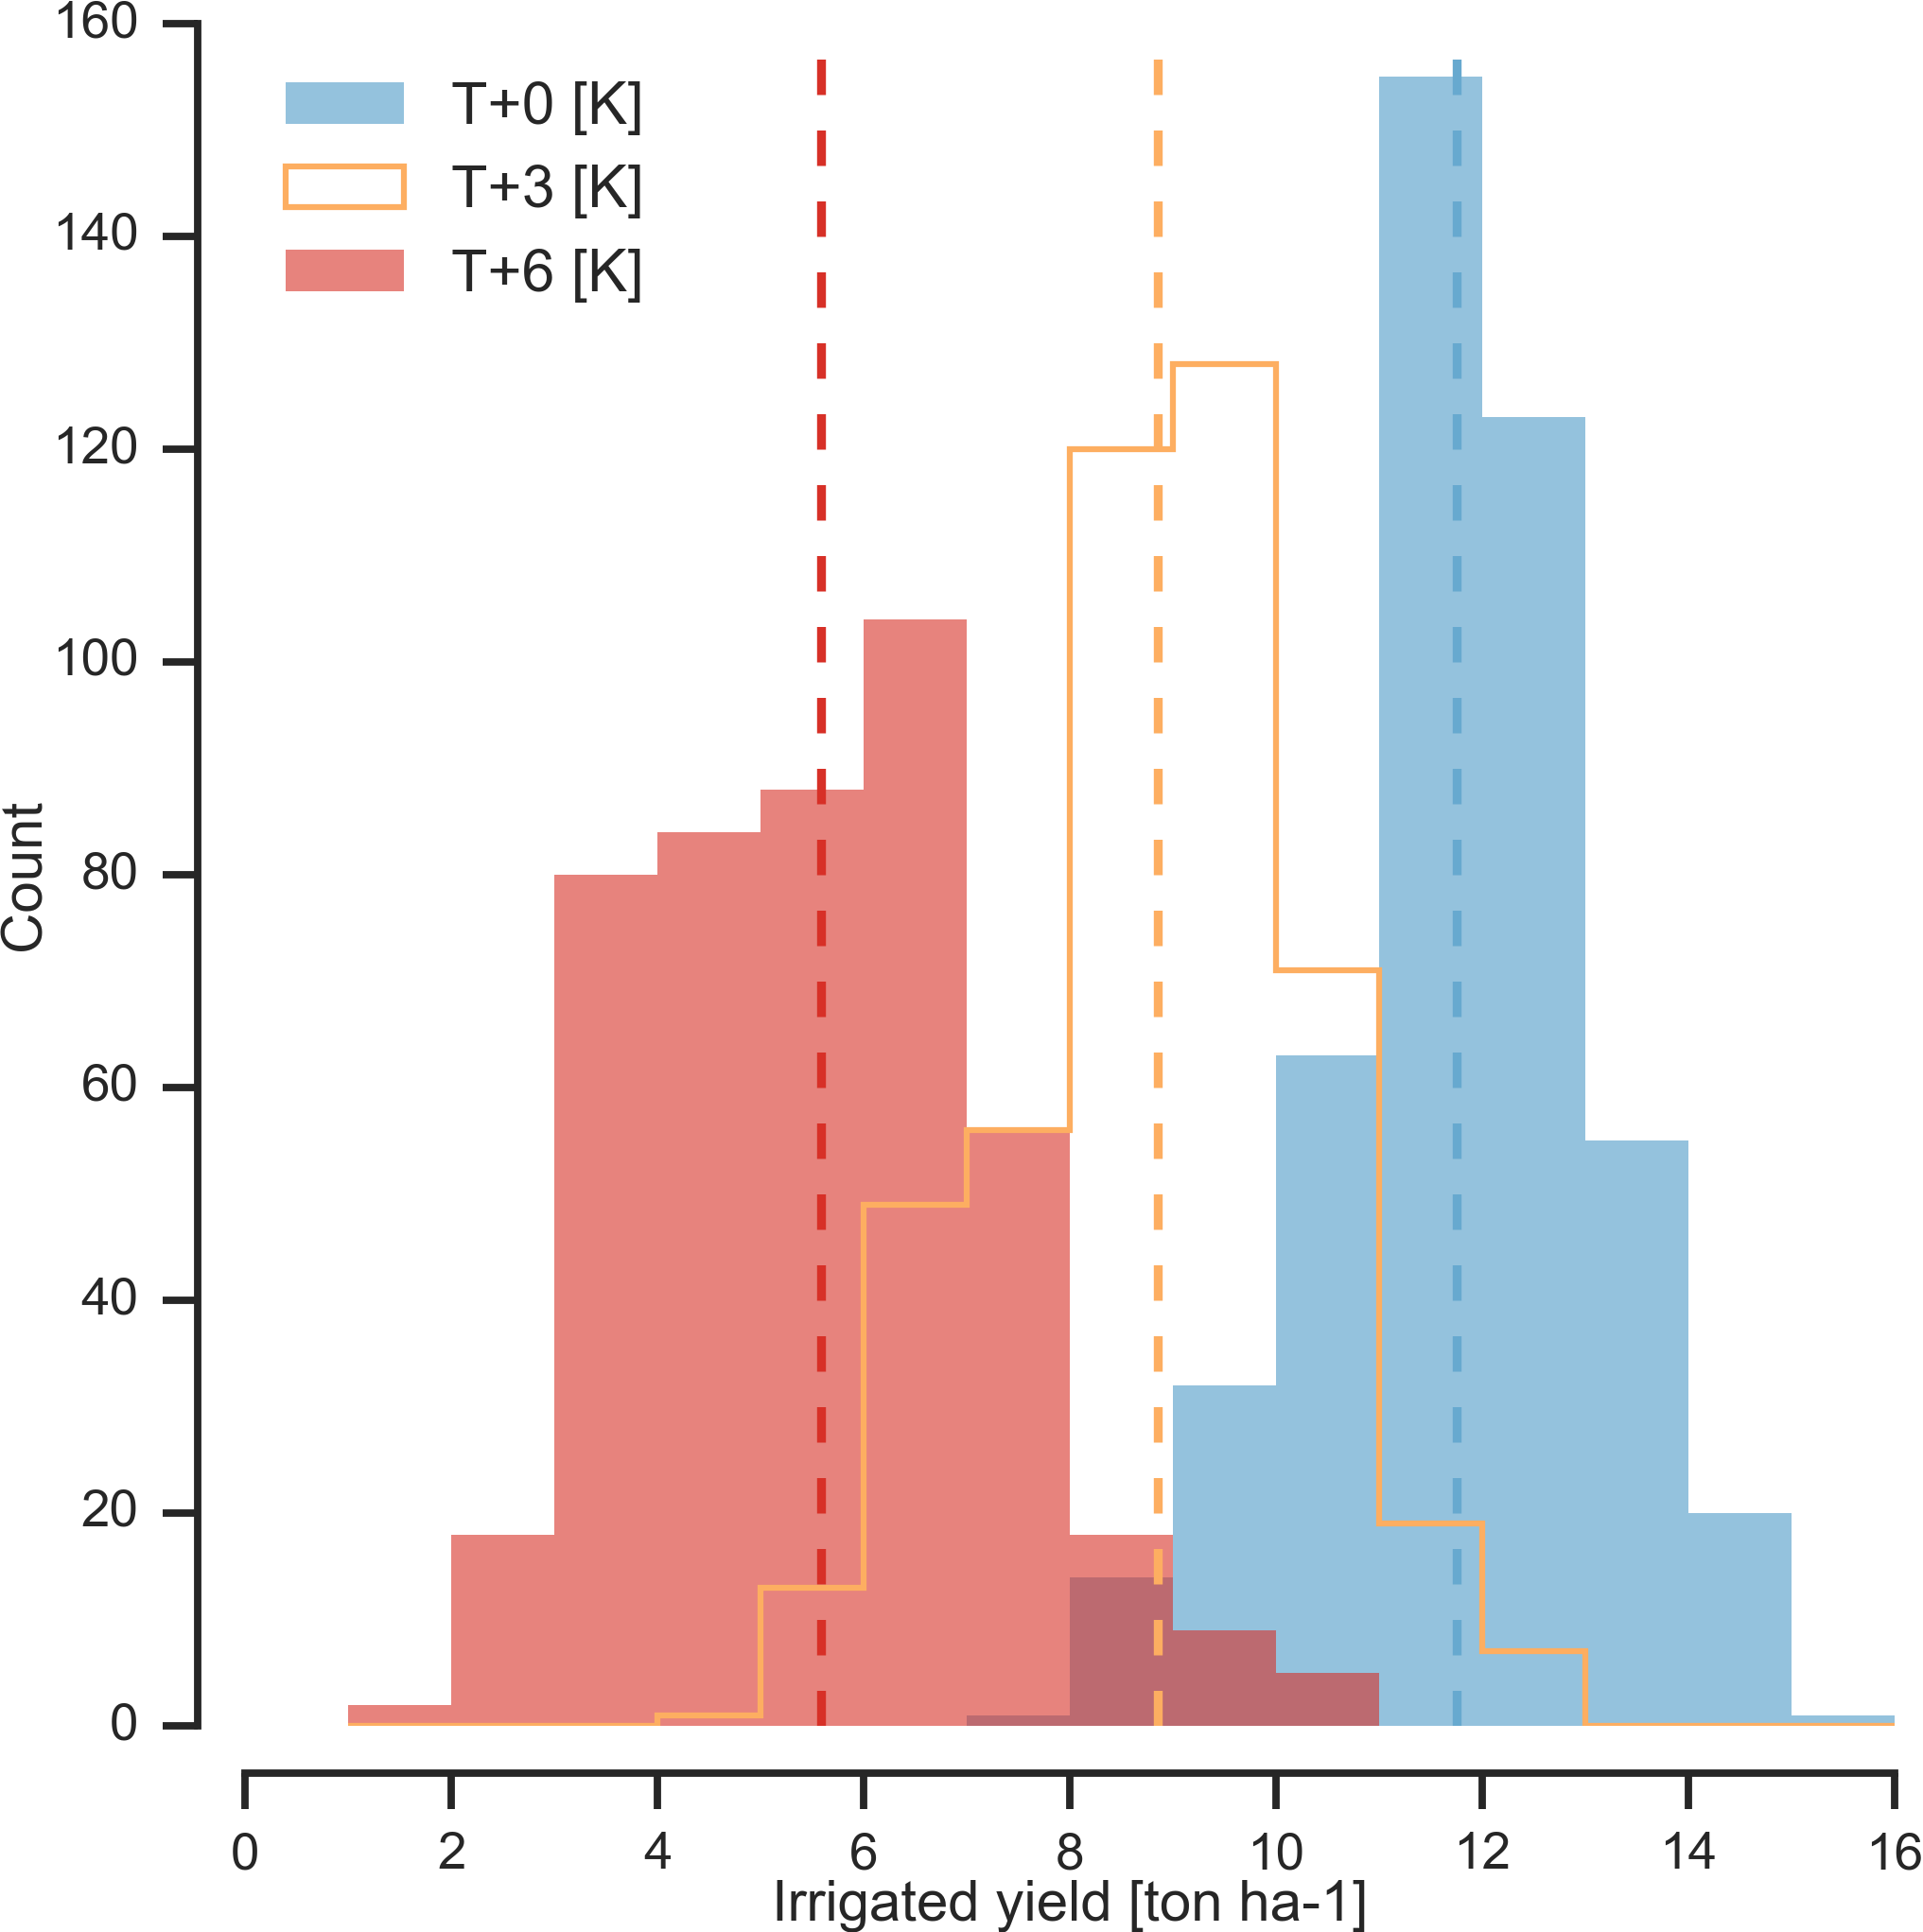
\includegraphics[width=7cm]{figures/hist_year_t.png} \hspace{10mm} 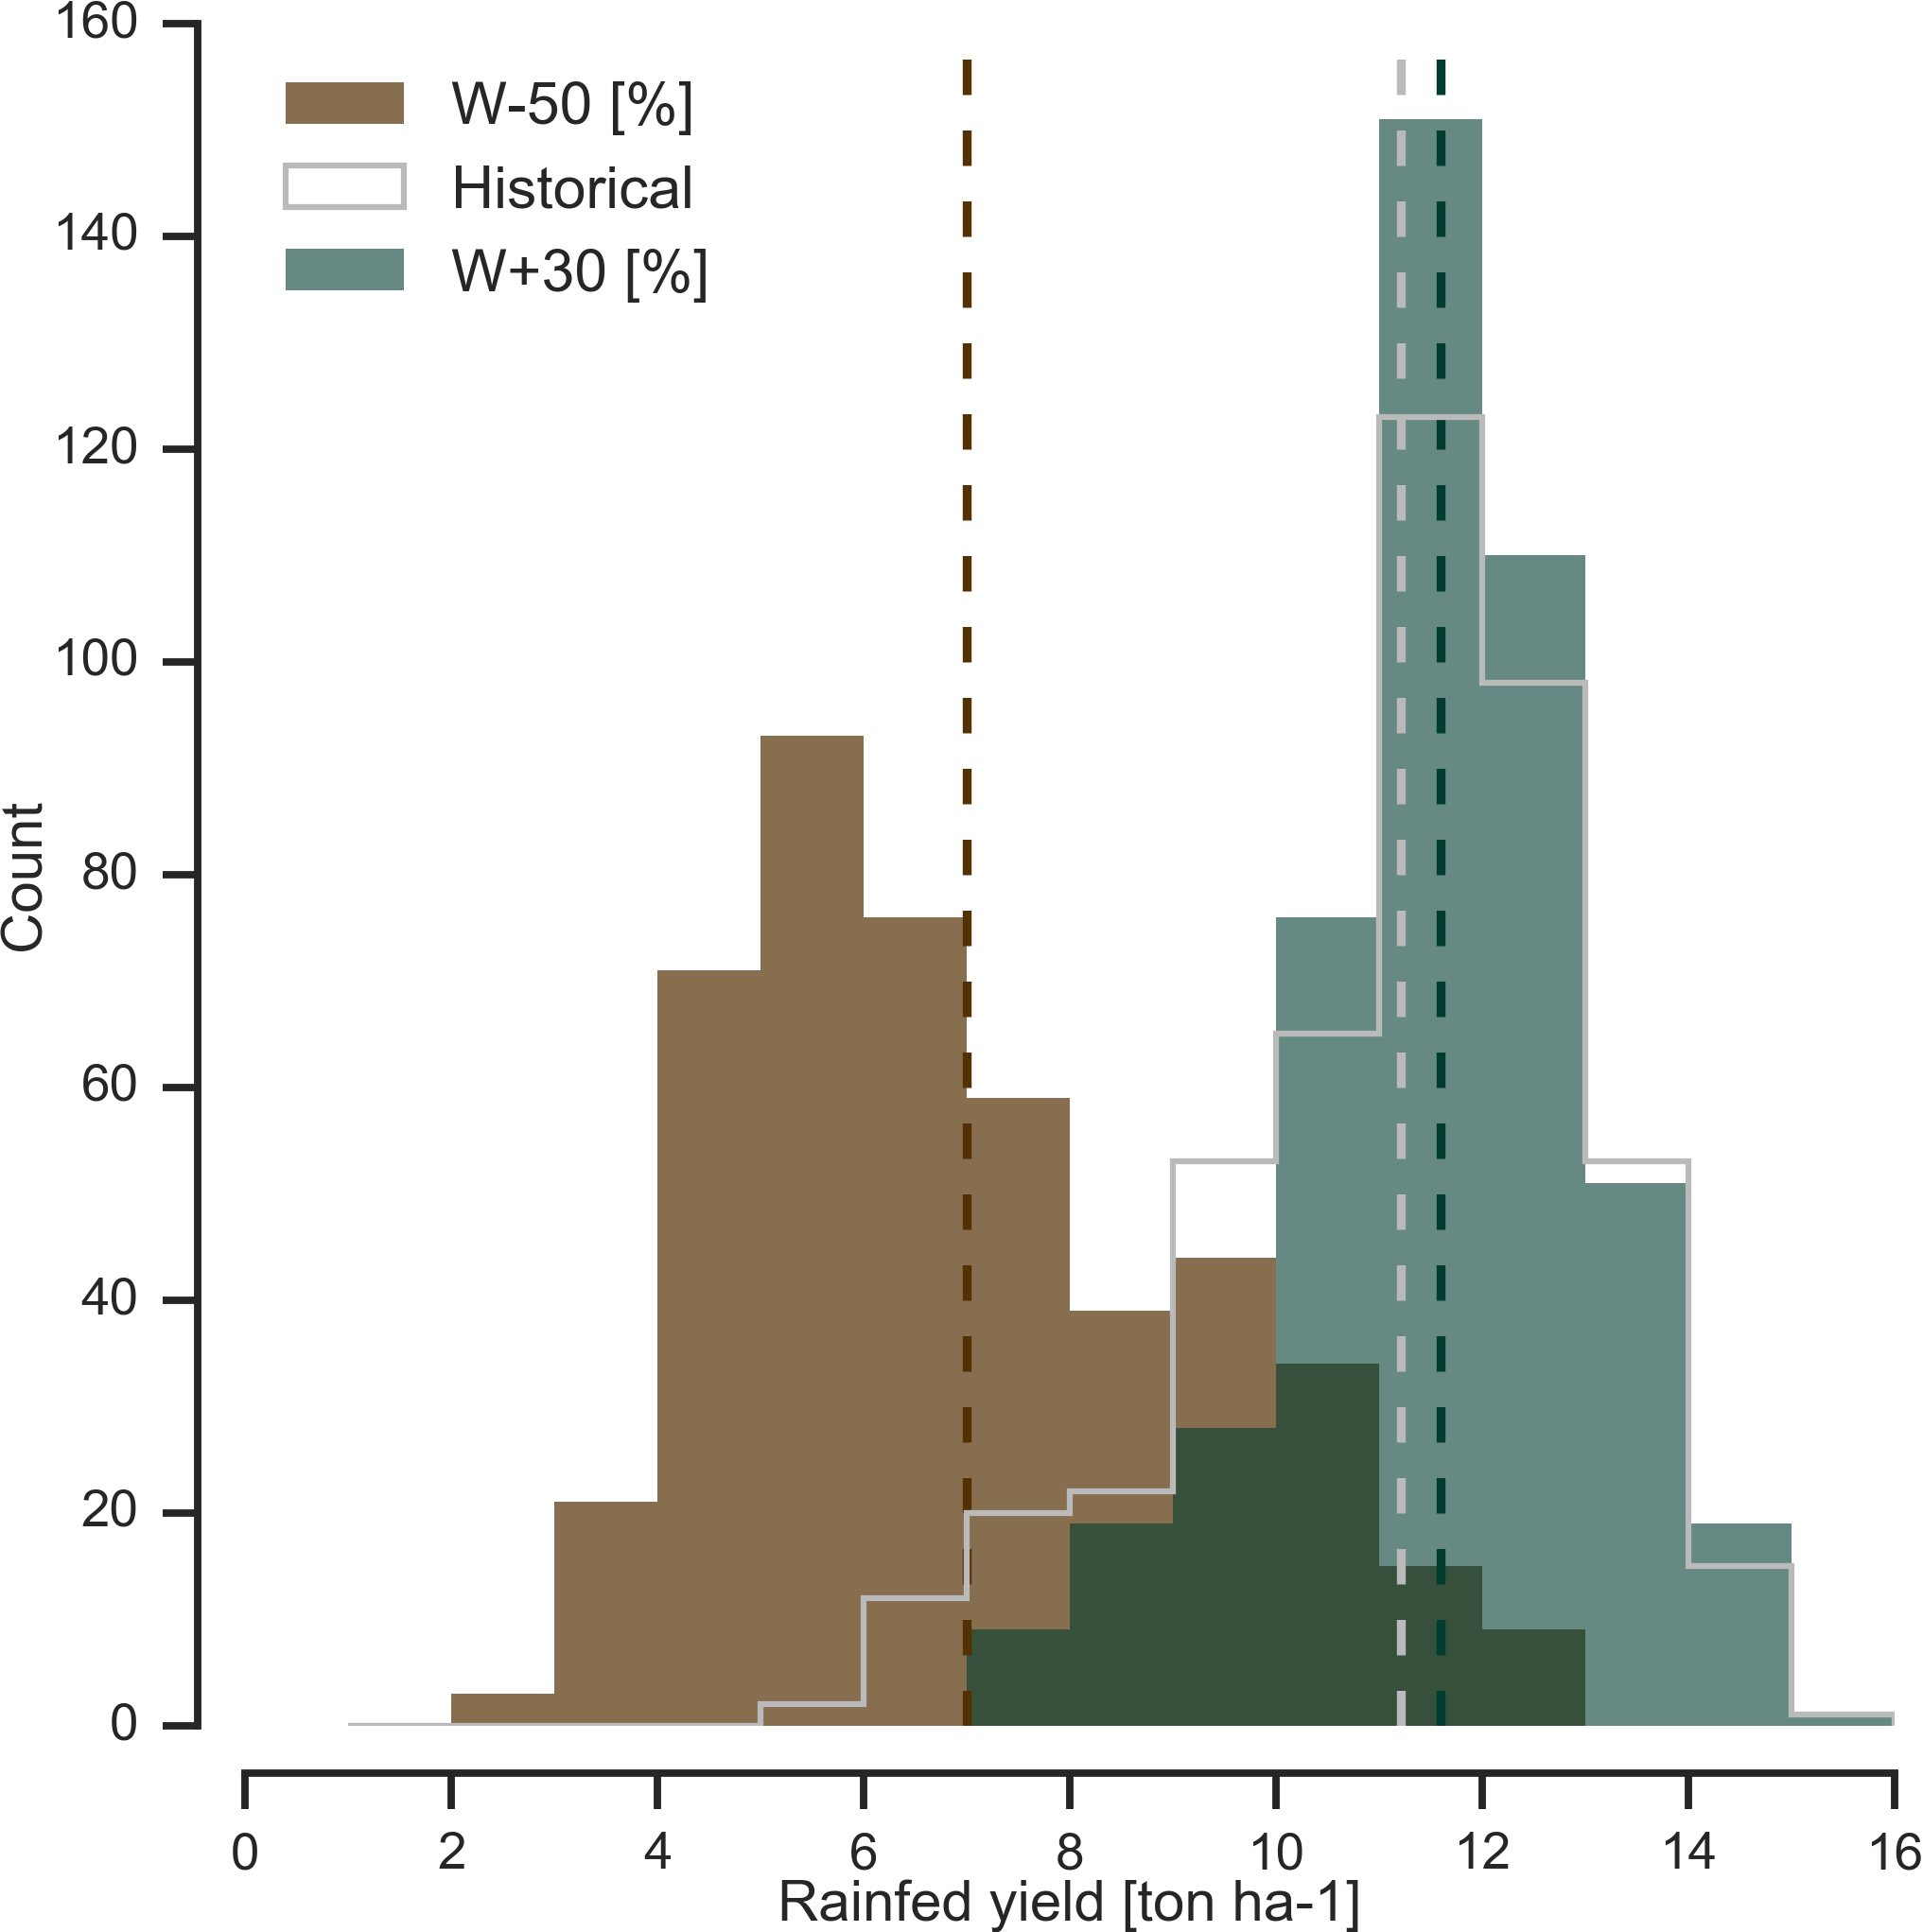
\includegraphics[width=7cm]{figures/hist_year_pr.png}
   \caption{
   Example showing results of increased crop yield sensitivity to year-over-year climate variations under climate stress. 
   Figure shows distributions of yields from examples of Figure \ref{fig:yearvclim}, of irrigated (left) and rainfed (right) maize in Iowa in scenarios of altered temperature (left) and precipitation (right).
   Under large warming (T+6) or drying (P-50\%), increased sensitivity means that distributions of year-over-year crop yields widen relative to present-day simulations, even though input climate has identical variance in climate drivers.
   }
   \label{fig:yearly}
\end{figure}

so the section on Figure 1 says, can year-over-year and climatological responses be different? the answer is sometimes yes. For example, in 
Figure 1 the year-over-year responses for temperature are very different from the climatological response. Both are approximately linear over the regime sampled, but different in slope, and and moreover the year-over-year response changes slope as a function of climate state). 
In the precip case, on the other hand, the climatological response is strongly nonlinear, but the year-over-year responses matches it very well. 
These effects are physically reasonable. Crops are very sensitive to daily temperature extrema and year-over-year and climatological changes in mean temperature can be associated with different changes (or lack of changes) in the growing season temperature distribution, and so produce different responses. 
Crops are less sensitive to short-term precipitation changes, since they care about soil moisture and the soil integrates.(cite Glotter et al for showing that in all but very arid regions, crop responses in models are not sensitive to how the precipitation is distributed within a month).

In both cases show in the Figure 2, the year-over-year response is nonlinear, getting stronger with more severe mean climate shifts. 
That strengthening of crop sensitivity means that under severe climate shifts, distribution of modeled crop yields becomes wider, even when underlying climate variability is the same (Figure 2). 
For temperature, that strengthening year-over-year response adds another complication to  emulating when using a non-stationary scenario where mean climate gradually warms.

I kind of feel that Figure 2 doesn't alone say anything about how hard the system is to emulate. In the precip case, the fact that the distribution widens is fine, because the climatological response is identical. It's only in the T case that it's a real problem. 
I'm sure fitting a strongly nonlinear response is hard anyway, but with precip in the example that you have, I don't think it gets harder by throwing in individual years.

%% XX -- this subsection not edited, make longer -- XX}
The first critical design choice for our emulators is centered around temporal aggregation.
We construct our emulator of 30-year climatological mean yields because most economic models project impacts at some aggregate temporal scale (decades or larger) or utilize some temporally aggregated climate projection as their input.
The GGCMI Phase II model experiment parameter sweep was designed to provide a training dataset for emulation that is structured in a way conducive to this temporal aggregation.

Three important distinctions are made between the year-to-year yield response and the climatological-mean yield response.
First, the year-over-year responses to weather are generally quantitatively distinct from (and, in the case of temperature, larger than) the climatological mean responses in the GGCMI Phase II simulation output dataset. 
In the example in Figure \ref{fig:yearvclim} for irrigated maize in Iowa, responses to year-over-year temperature variations are 100\% larger than those to long-term perturbations in the baseline case, and larger still under warmer conditions, rising to nearly 200\% more in the T+6 case. 
The same general principal applies to the precipitation dimension however in this case it is more manifestly an artifact of sampling range in the historical period (Figure \ref{fig:yearvclim}, right).
Year-over-year and climatological responses can differ for many reasons including memory in the crop model, lurking covariates, and differing associated distributions of daily growing-season daily weather \citep[e.g.][]{Ruane2016}. 

Second, the year-over-year response is not constant across different levels of climate stress. 
For example, the stronger year-over-year response to temperature under warmer conditions also manifests as a wider distribution of yearly yields (Figure \ref{fig:yearly}) within a 30-year simulation even though the variance in input temperates is unchanged. 
Likewise for precipitation changes, strong decreases in precipitation results in a widening of the distribution in yields even though the variance in precipitation is decreasing (from approximately 60 cm yr-1 to 30 cm yr-1 in this example). 
\textcolor{red}{...both are manifestations of the non-linear mapping from input weather to yields}
Since we emulate mean climatological-yields, we do not capture any of these higher-order moment changes in yield in this study.

Finally, the climatological-mean yield response is considerably smoother than the year-to-year yield response and makes emulation relatively simple. 
Note that the GGCMI Phase II training dataset does not capture potential changes in climate variability, because all simulations are run with fixed offsets from the historical climatology.
However, prior work has suggested that mean changes are the dominant drivers of climatological crop yield shifts in all but arid regions \citep[e.g.][]{Glotter14}.
Critically for emulation, the mean-climatological yield can easily be related to the mean-climatological shift in temperature or precipitation in the GGCMI Phase II dataset.

%%%%%%%%%%%%%%%%%%%%%%%%%%%%%%%%%%%%%%%%%%%%%%%%%%%%
\section{Emulation}
\label{S:3}
Emulation involves fitting individual regression models from GGCMI Phase II output for each crop and model and 0.5 degree geographic pixel; the regressors are the applied perturbations in CO$_2$, temperature, water, and nitrogen (CTWN). 
We discuss here largely emulations of climatological mean crop yield with no growing season adaptation (A0 scenarios), but note that any output of the crop models can potentially be emulated. 
We provide separate emulations of not only irrigated and rainfed yields but also irrigation water demand in both the A0 and A1 growing season, meaning that each model and crop combination results in six regressions. (See Supplementary Material XX for more information on additional cases not shown.)

\subsection{Statistical model} %Feature engineering}
For the statistical model of crop yields as a function of CTWN, we choose a relatively simple parametric model with a 3rd-order polynomial basis function. 
If the climatological mean response is relatively smooth, then a simpler form provides a reasonable fit that allows for some interpretation of resultant parameter weights. 
A relativity simple parametric form also allows fast model emulation at the grid cell level as opposed to the global or large regional level. 
By emulating at the grid cell level, we indirectly includes any yield response to geographically distributed factors such as soil type, insolation, and the baseline climate, and preserve the spatial resolution of the parent models.
To facilitate potential parameter-by-parameter comparison across crop models, we hold the functional form constant in space, across all crops, and models. 
That is, the same statistical model is used for all grid cells, models, and rainfed crops. 
(Note however that regressions for irrigated crops do not contain W terms and models that do not sample the nitrogen levels omit the N terms.)

Both higher-order and interaction terms are expected to be important for representing crop yields. Higher order terms are needed because crop yield responses to weather are well-documented to be nonlinear: e.g.\ \citet{Schlenker2009} for T perturbations and \citet{He2016} for W (precipitation). 
%The mean-climatological response is relatively smooth but also manifestly non-linear.
Interaction terms are needed since the yield response is expected to depend on interactions between the major inputs. 
For example, \citet{Lobell2007} and \citet{Tebaldi2008} showed that in real-world yields (with C and N fixed), the joint distribution in T and W is needed to explain observed yield variance.  
Other observation-based studies have shown the importance of the interaction between W and N \citep[e.g.][]{AULAKH2005}, and between N and C \citep{Mitsuru92, Nakamura97}. 

A full third order polynomial with interaction terms for the four regressors (CTWN) has 34 total terms (Equation \ref{eqn:features_original}), too many for robust fitting even with the large GGCMI Phase II dataset. %The large GGCMI Phase II sampled variable space greatly aids in fitting statistical models, but it is still sufficiently limited that use of the full 34-parameter polynomial basis function can be problematic.
We therefore reduce the number of free parameters through a feature selection process (discussed in detail below), eliminating 10 terms that do not play a significant role in predicting crop yields; these are shown in {\color{dark-gray}gray} in Equation \ref{eqn:features_original}. 
The resulting 23-parameter model can be well-fitted to crop model response in nearly all regions, with the only exceptions being extremely low-yield regions where crops are not currently grown.

\begin{align}
    \label{eqn:features_original}
    Y\ = \ & K_{1}  \\
    + \ & K_{2} C      + K_{3} T      + K_{4} W      + K_{5} N   \nonumber \\
    + \ & K_{6} C^2    + K_{7} T^2    + K_{8} W^2    + K_{9} N^2 \nonumber \\
    + \ & K_{10} C W   + K_{11} C N   + K_{12} T W   + K_{13} T N   + K_{14} W N \nonumber \\
    + \ & {\color{dark-gray}K_{a} C T} + K_{15} T^3  + K_{16} W^3  + {\color{dark-gray}K_{b} C^3} + {\color{dark-gray}K_{c} N^3} \nonumber \\
    + \ & K_{17} T W N + K_{18} T^2 W + K_{19} W^2 T + K_{20} W^2 N + {\color{dark-gray}K_{d} C W N} \nonumber \\
    + \ & {\color{dark-gray}K_{e} C T N} + K_{21} N^2 C + K_{22} N^2 T + K_{23} N^2 W + {\color{dark-gray}K_{f} T^2 N} \nonumber \\
    + \ & {\color{dark-gray}K_{g} T^2 C} + {\color{dark-gray}K_{h} W^2 C} + {\color{dark-gray}K_{i} C^2 W} + {\color{dark-gray}K_{j} C^2 T} + {\color{dark-gray}K_{k} C^2 N} \nonumber
\end{align}

We do not focus in this study on comparing different functional forms or non-parametric models.
Some prior studies have used other statistical specifications in crop model emulation: for example, \citet{BLANC2015} and \citet{BLANC2017} use a 39 term fractional polynomial. 
Such a high-dimensional model is difficult to fit, especially for a training set of realistic simulations in which input parameters are highly correlated, and  \citet{BLANC2015} and \citet{BLANC2017}  ``borrow information across space'' by fitting grid points simultaneously across soil region in a panel regression. 
Our simpler functional form can be fit independently at each grid cell while still providing a satisfactory emulation of all GGCMI crop models and crops. 
(See Section \ref{S:4} for evaluation of emulator fidelity.)

\subsection{Feature selection} %Regularization}
%The large GGCMI Phase II sampled variable space greatly aids in fitting statistical models, but it is still sufficiently limited that use of the full 34-parameter polynomial basis function described above can be problematic.
To reduce the number of terms in our statistical model, we apply a feature selection cross-validation process in which terms in the polynomial are tested for importance.
In this procedure higher-order and interaction terms are added successively to the regression model one by one, and 
we calculate an aggregate mean absolute error with each increasing terms and eliminate those terms that do not contribute significant reductions in error (top row of Figure \ref{fig:features}). 
Some terms that did not reduce the aggregate error are included if a higher order version of that term provided a decrease in mean squared error: for example, the $T^3$ term cannot be included without also taking the $T^2$ and $T$ terms. 
We select terms by applying the feature selection process to three example models: two that provided the complete set of 672 rainfed simulations (pDSSAT, EPIC-TAMU, and one that provided the smallest training set (120, PEPIC). 
Feature importance is not uniform due to spatial heterogeneity across models and crops, so we weight the loss function by current cultivation area during this step. 
The resulting choice of terms is then applied for all emulators and all crops. 
Since the goal of the emulator is interpolation within the sample space and not extrapolation, we err on the side of including terms that are useful in at least some cases, because the added predictive ability outweighs the costs to distribution of the residuals or over fitting.  

\begin{figure*}[ht]
\centering
   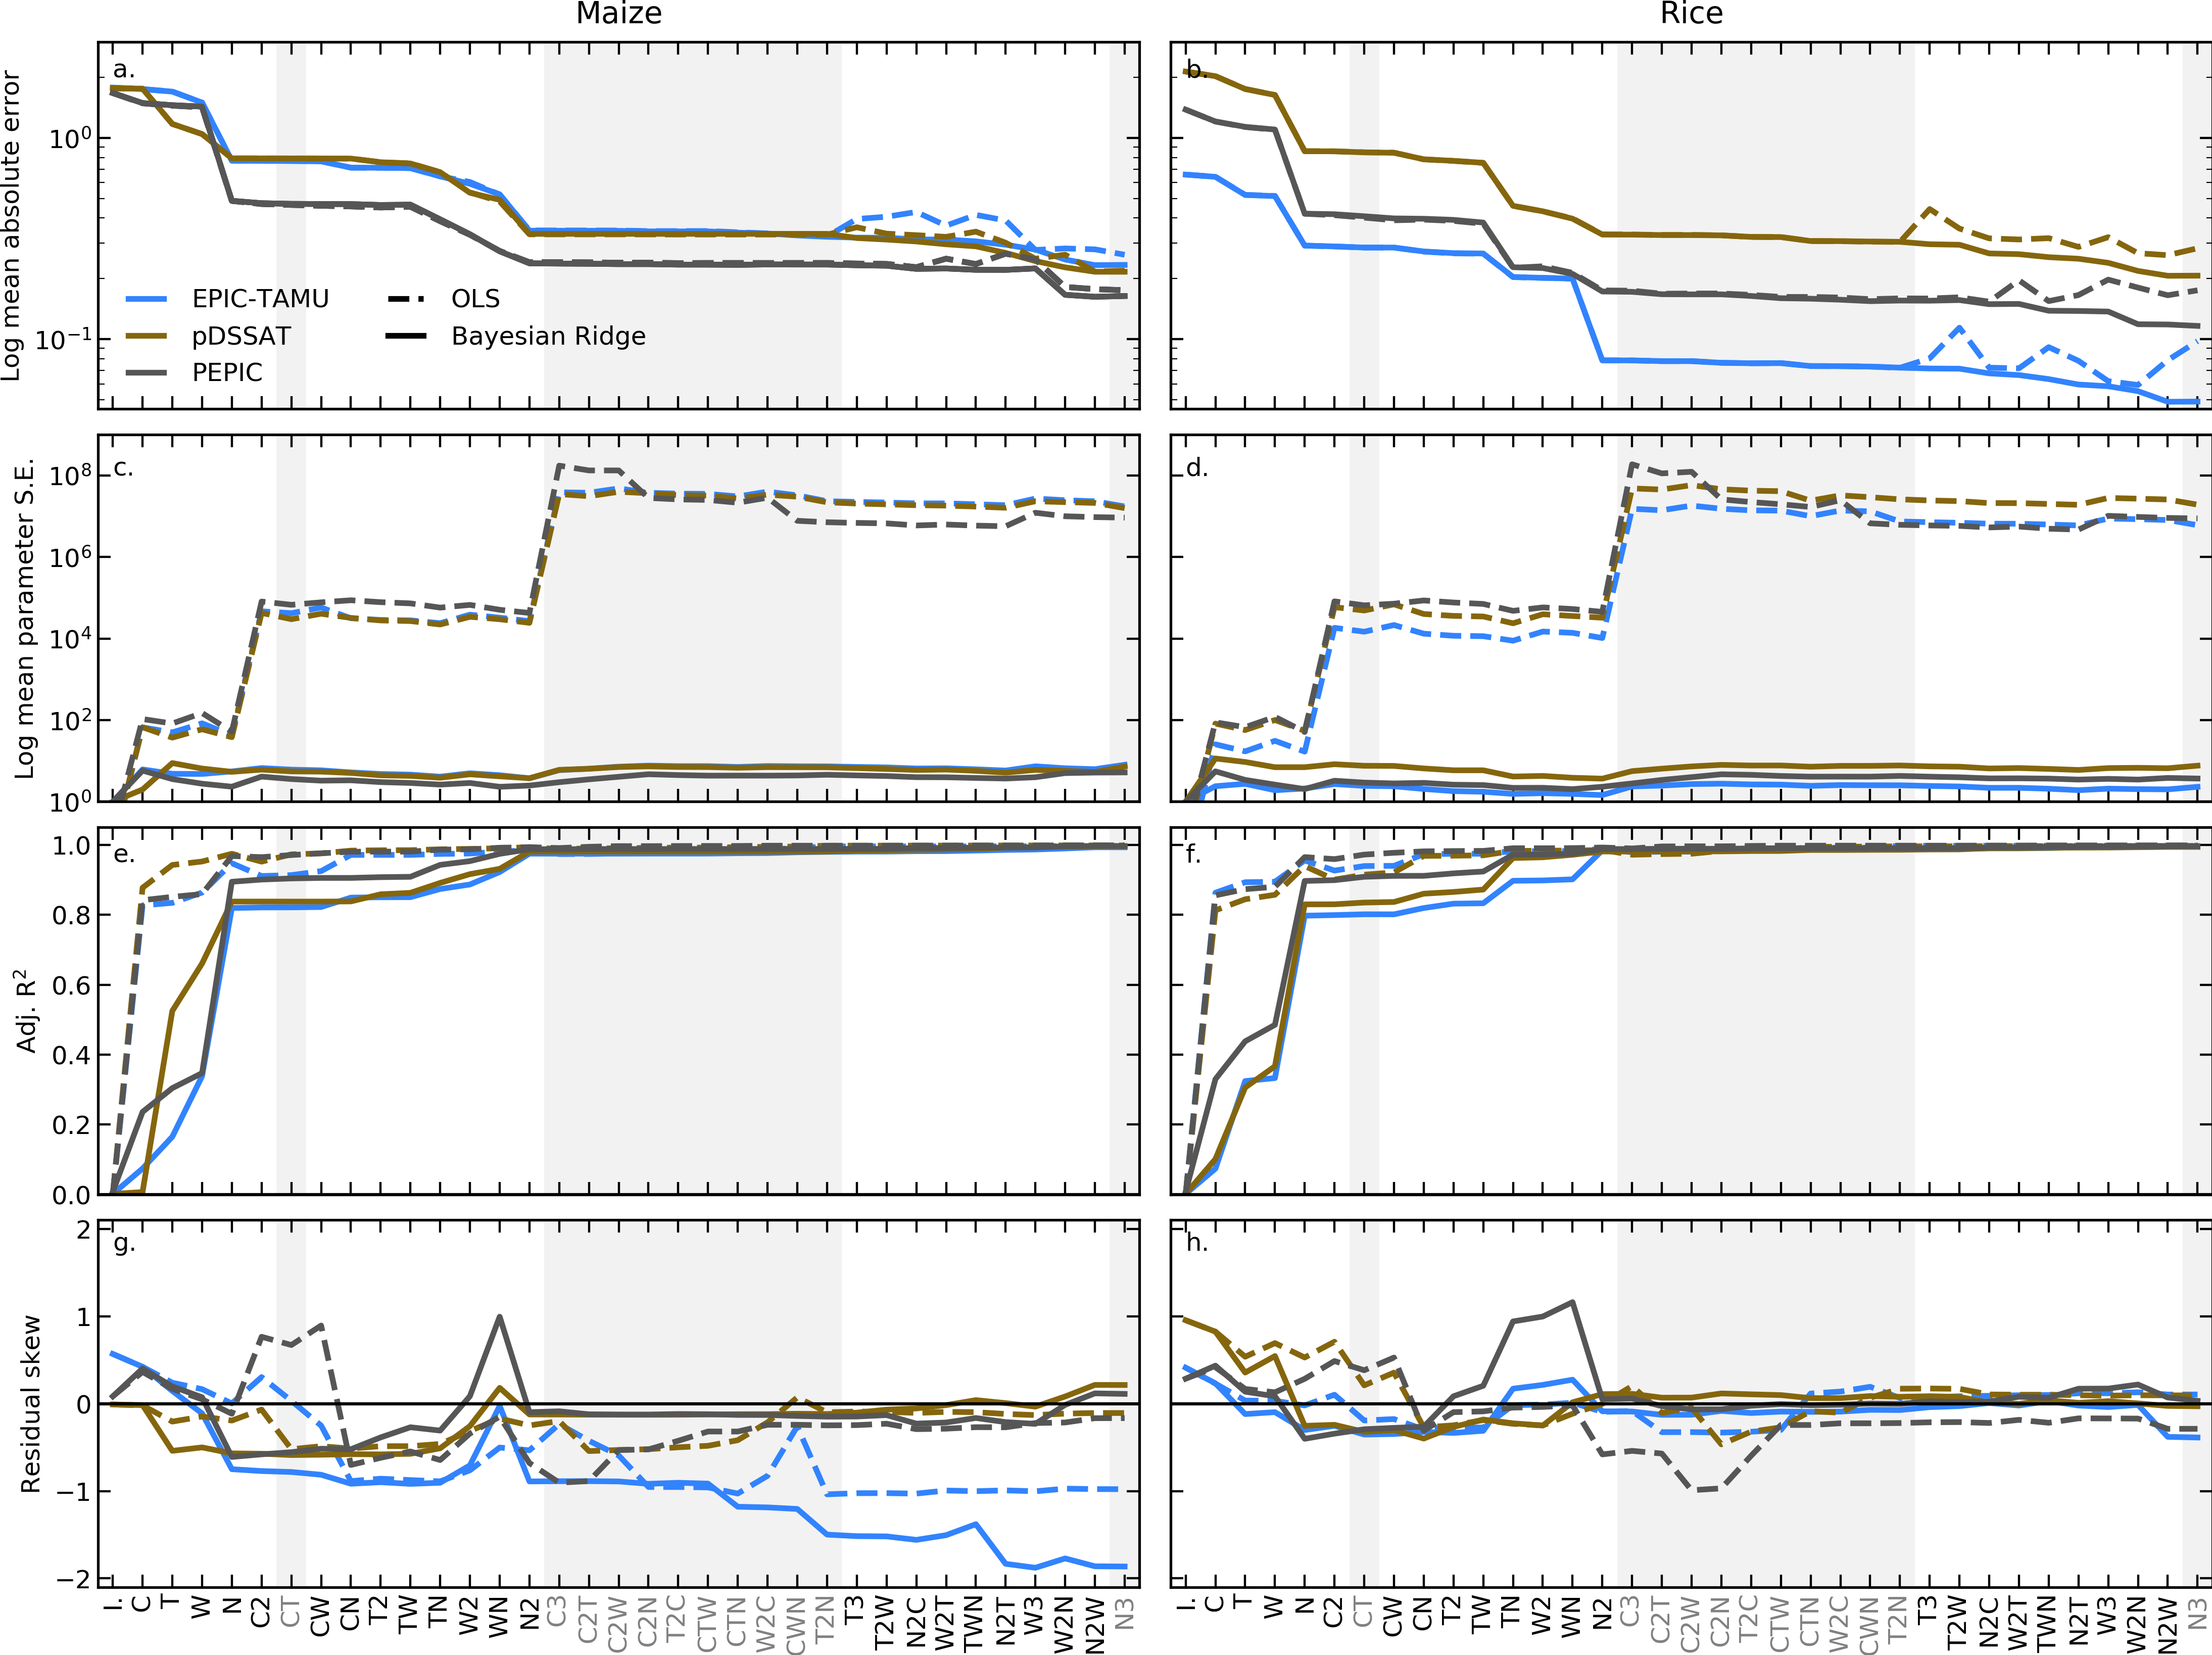
\includegraphics[width=12cm]{figures/model_select_maize_rice.png}
   \caption{Summary results from polynomial feature selection process.
   The top row illustrates log mean absolute error between emulated yield and simulated values calculated with a three fold cross validation process, where the emulator is trained on two thirds of the data and predicts the remaining third.
   The second row illustrates the adjusted R$^2$ score for the fit at each model specification where additional terms are penalized.
   The third row illustrates the log mean standard parameter error and the forth and fifth rows illustrate the distribution of the residuals.
   The X- axis indicates terms included in the model at each step progressively where T = temperature, T2 = temperature$^{2}$, TW  = temperature * water and so on. 
   The terms that did not reduce the aggregate error (horizontal lines) are not included in the final model. 
   Solid lines indicate Bayesian Ridge regression results and dashed lines indicated standard ordinary least squares. 
   Colors indicated three different crop models.}
   \label{fig:features}
\end{figure*}

Feature importance is remarkably consistent across models (Figure \ref{fig:features}). 
Even though the models exhibit different absolute levels of error, all three models agree remarkably well on feature importance indicated by the terms where the error is reduced and where additional terms provide no predictive benefit (line slopes match in Figure \ref{fig:features}). 
The feature selection process results in a final polynomial in 23 terms, with 11 terms eliminated. 
We omit the N$^3$ term, which cannot be fitted because we sample only three nitrogen levels. 
We eliminate many of the C terms: the cubic, the CT, CTN, and CWN interaction terms, and all higher order interaction terms in C. 
Finally, we eliminate two 2nd-order interaction terms in T and one in W. 
Implication of this choice include that nitrogen interactions are complex and important, and that water interaction effects are more nonlinear than those in temperature. 

\subsection{Model fitting}
To fit the parameters $K$, we use a Bayesian Ridge regularization method \citep{MacKay91}, which reduces volatility in parameter estimates when the sampling is sparse, by weighting parameter estimates towards zero. 
The choice results in a reduction in mean absolute error for some of th high-order interaction terms in the model (top row of Figure \ref{fig:features}) and drastically reduces standard parameter error in the model by stabilizing the estimates.
The estimation method scores relatively lower on adjusted $R^2$ (equation \ref{eqn:rsquare}, where $n$ is the number of samples and $k$ is the number of features) for the simplest parameter specifications, but reaches parity with the OLS at the number of terms included in this study.
The Bayesian Ridge method is necessary over the standard OLS to maintain a consistent functional form across all models and locations (see Table \ref{table:ASE}). 

\begin{equation}
    \label{eqn:rsquare}
    R^{2}_{adj} = 1 - \frac{(n-1) \cdot (1 - R^{2})}{n - k}
\end{equation}

The distribution of the residuals depends on the number of features included in the regression, the method for estimating the parameters, and the target distribution in the training set. 
Including additional higher order terms in the model tends to reduce the skew in the residuals in most cases.
The residuals are only normally distributed (Shapiro–Wilk test \citep{Shapiro1965} pvalue > 0.05) for one of the crop models shown in Figure \ref{fig:features} for any specification tested.
The EPIC-TAMU and pDSSAT crop module emulator residuals are never normally distributed by this metric for any feature specification proposed here. 

We use the implementation of the Bayesian Ridge estimator from the scikit-learn package in Python \citep{scikit-learn}. 
In the GGCMI Phase II experiment, the most problematic fits are those for models that provided a limited number of cases or for low-yield geographic regions where some modeling groups did not run all scenarios. 
We do not attempt to emulate models that provided less than 50 simulations. 
The lowest number of simulations emulated across the full parameter space is then 120 (for the PEPIC model). 

%%%%%%%%%%%%%%%%%%%%%%%%%%%%%%%%%%%%%%%%%%%%%%%%%%%%%%%%%%%%%%%
%%%%%%%%%%%%%%%%%%%%%%%%%%%%%%%%%%%%%%%%%%%%%%%%%%%%%%%%%%%%%%%
%%%%%%%%%%%%%%%%%%%%%%%%%%%%%%%%%%%%%%%%%%%%%%%%%%%%%%%%%%%%%%%
\section{Emulator evaluation}
\label{S:4}
In the following section we present some illustrations of emulator performance.
Model emulation with the parametric method used here is only possible when the crop yield responses are sufficiently smooth and continuous to allow fitting with a relatively simple functional form, but this condition largely holds in the GGCMI Phase II simulations. 
However, the principle of no-free-lunch applies, so losses between the emulator and simulations are great enough to be problematic in certain cases, especially for models with limited sampling or in geographic locations where crops are currently not grown. 
The errors between the simulation and the emulation are generally small compared to the difference across different crop models or across the response to different climate model inputs.

\subsection{Emulator behavior}
\begin{figure*}[ht]
\centerings
    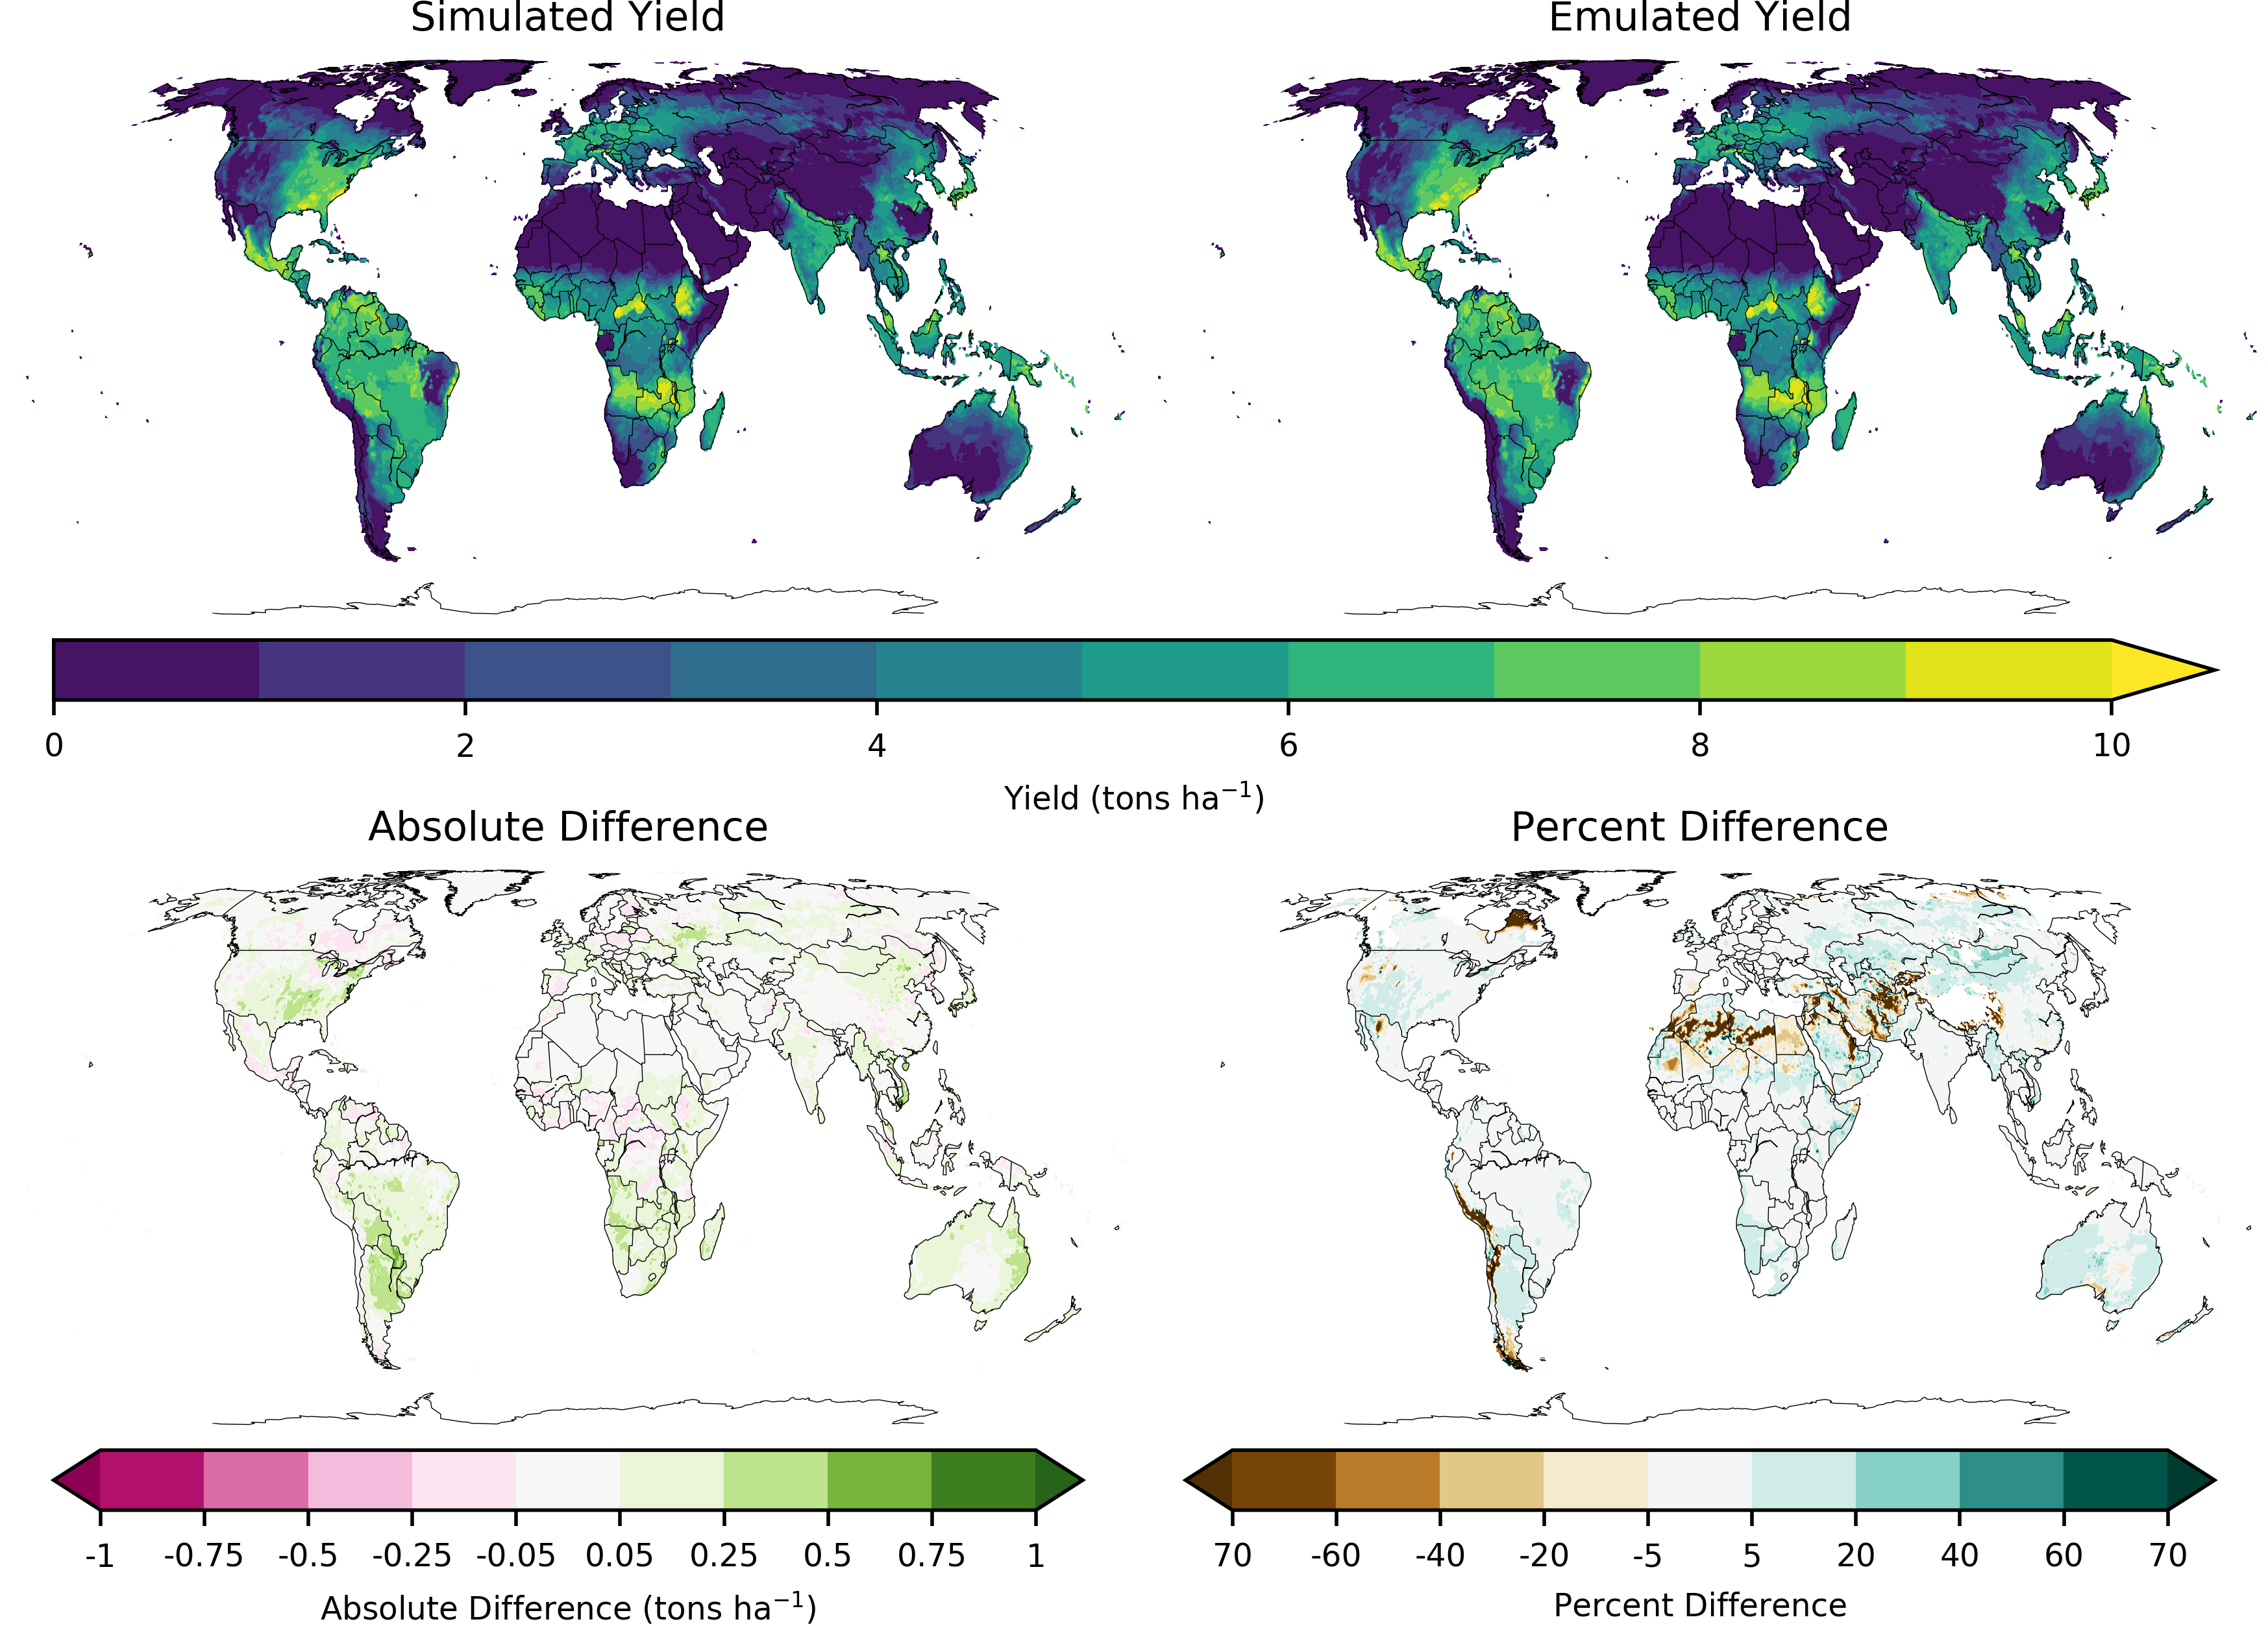
\includegraphics[width=16cm]{figures/lpjml_maize.png}
    \caption{Illustration of spatial pattern in baseline yield successfully captured by the emulator.
    Simulated and emulated yield under historical (1981-2010) conditions for rainfed maize from the LPJmL model.
    Absolute yield differences are less that 0.5 ton ha$^{-1}$ in almost all (99.8\%) grid cells across the globe.
    Percent differences (from simulated baseline) is below 5\% in most (75\%) grid cells currently cultivated in the real world.
    Approximately 7\% of grid cells have errors over 20\% different from baseline, but only 3\% of grid cells with current cultivation \citep{Portmann2010} have errors over 20\%.
    Notable exceptions include areas with very low baseline yield in the simulations including, for example, the Sahara, the Andes, and northern Quebec. 
    Percent error weighted by cultivation area globally is essentially zero (see also Table \ref{table:ASE}).
    Performance varies by crop and model. 
    See supplemental for more examples.
    }
   \label{fig:map_pattern}
\end{figure*}

\begin{figure*}[ht]
\centering
    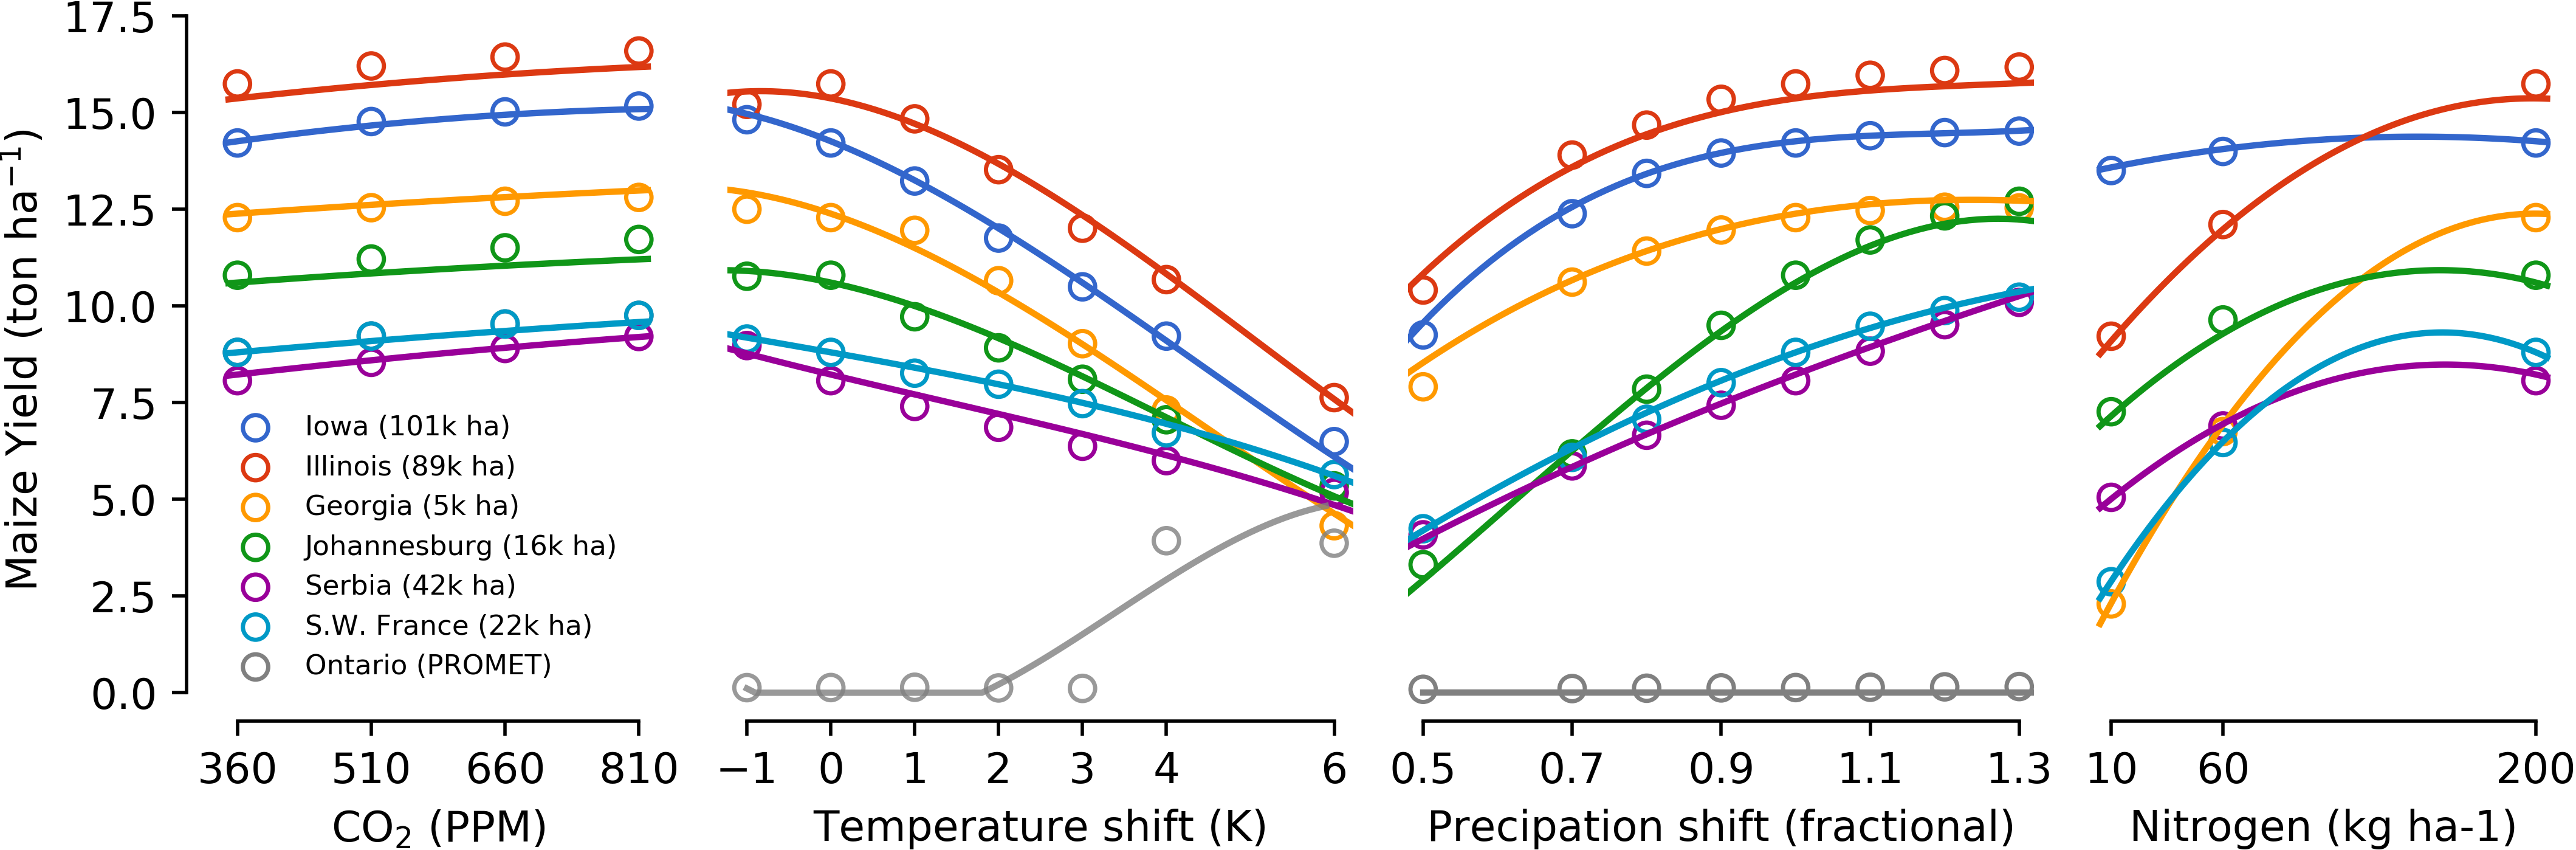
\includegraphics[width=16cm]{figures/regression_example_1.png}
    \caption{Illustration of spatial variations in yield response successfully captured by the emulator. 
    Figures show rainfed maize in the pDSSAT model in six example locations selected to represent high-cultivation areas around the globe. 
    Legend includes hectares cultivated in each selected grid cell. 
    Each panel shows variation along a single variable, with others held at baseline values. 
    Dots show climatological mean yields and lines the results of the full 4D emulator of Equation \ref{eqn:features_original}. 
    In general the climatological response surface is sufficiently smooth that it can be represented within the sampled variable space by the simple polynomial used in this work. 
    Extrapolation can however produce misleading results. 
    The rainfed maize response in north-central Ontario is shown for the PROMET model as a good example of an area where the emulator fails.
}
   \label{fig:regression}
\end{figure*}

\begin{figure*}[ht]
\centering
    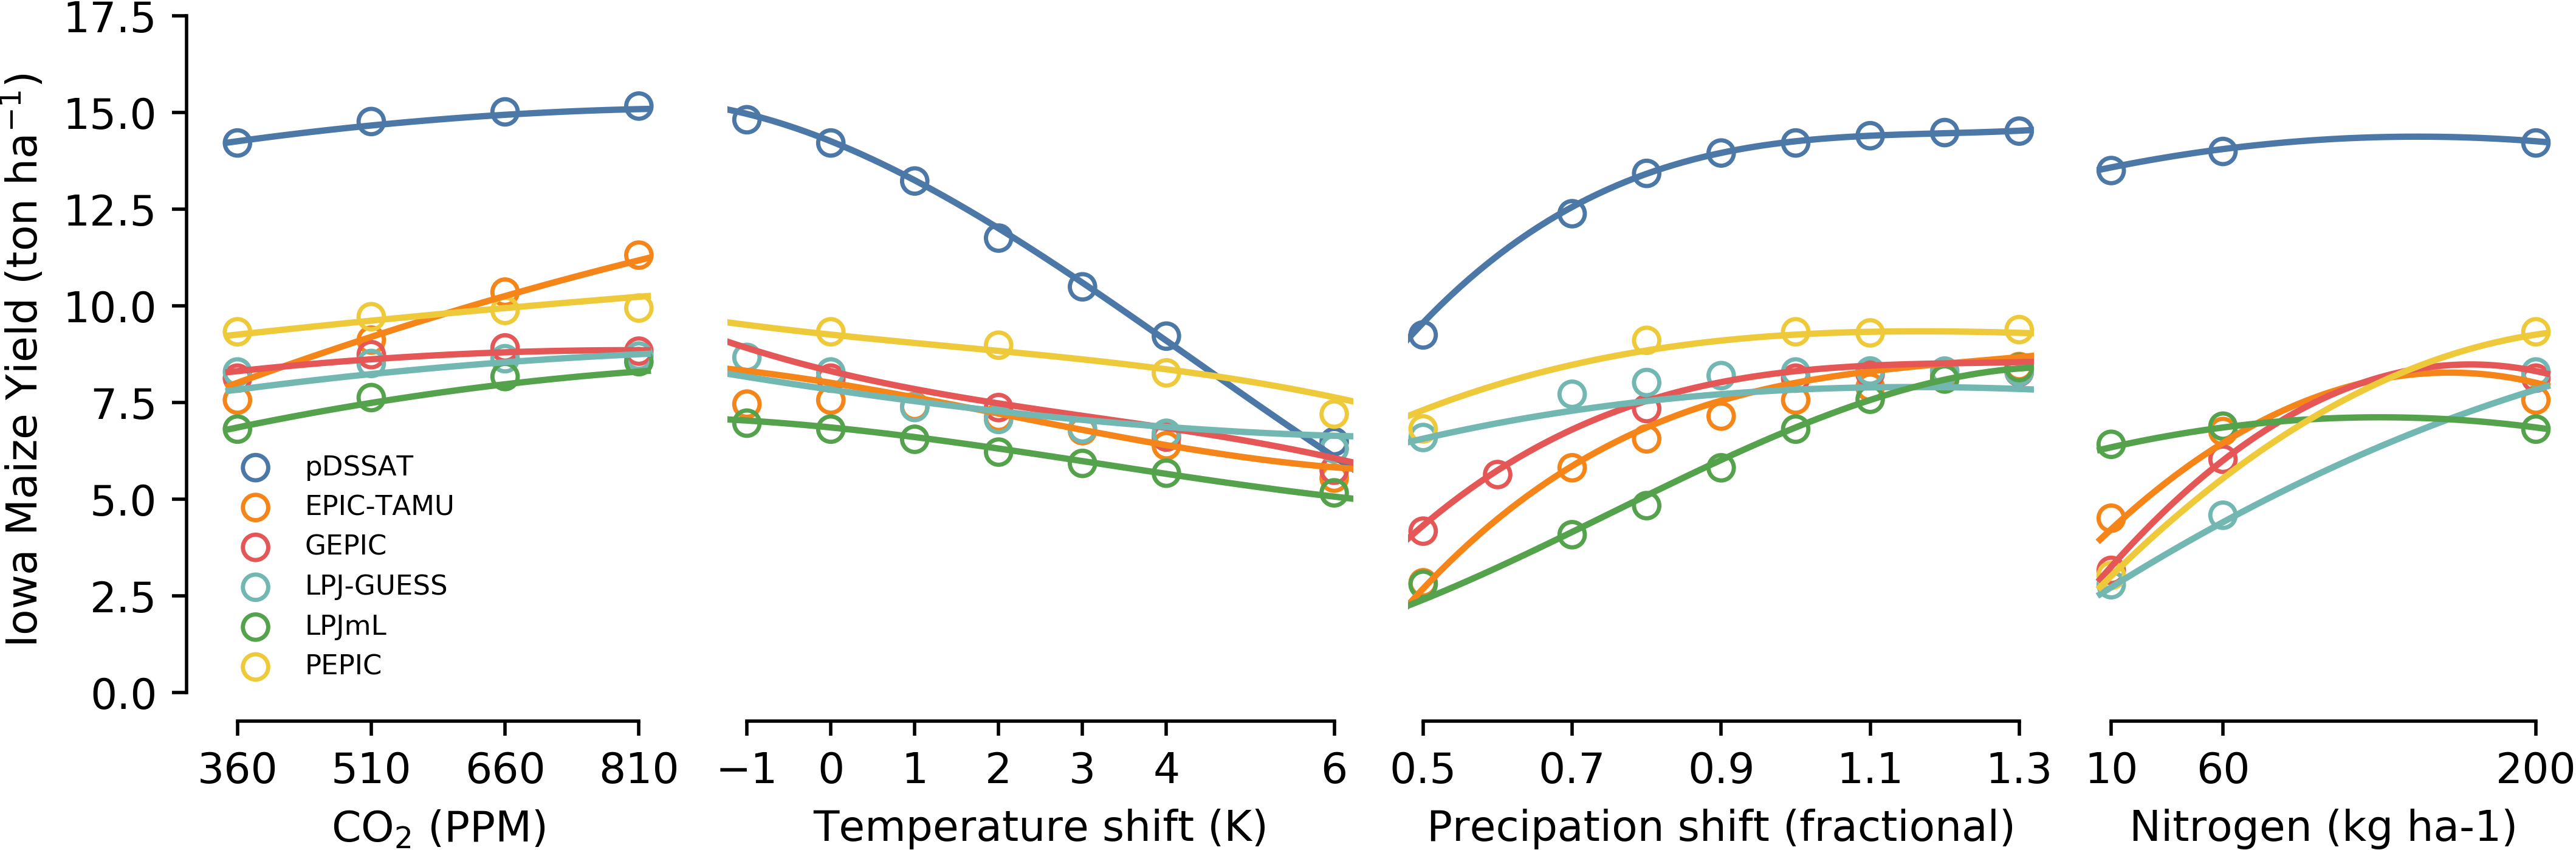
\includegraphics[width=16cm]{figures/regression_example_2.png}
    \caption{Illustration of across-model variations in yield response successfully captured by the emulator. 
    Figures shows simulations and emulations from six models for rainfed maize in the same Iowa grid cell shown in Figure \ref{fig:regression}, with the same plot conventions. 
    Models that do not simulate the nitrogen dimension are omitted for clarity. 
    Note that models are uncalibrated, increasing spread in absolute yields. 
    While most model responses can readily emulated with a simple polynomial, some response surfaces diverge slightly from the polynomial approach (e.g.\ LPJ-GUESS here) and lead to emulation error, though error generally remains small relative to inter-model uncertainty. 
    }
   \label{fig:regression_2}
\end{figure*}

The emulator is able to successfully capture the spatial pattern of yields for a single simulation case and emulation errors are low in regions currently under cultivation (Figure \ref{fig:map_pattern}). 
Nearly all grid cells have errors below 0.5 ha$^{-1}$ for the baseline case. 
However, emulation errors as a percentage of baseline yield does reach high values in some areas with no cultivation in the real world.
Many of these regions are not currently viable for agriculture and therefore have very low simulated baseline yields and may never become viable even under extreme climate change.  
Some differences in spatial skill exist across models and crops, with maize being the qualitatively easiest to emulate. 
See supplemental figures SXX-SXX for more crops and models. 

Yield responses are quite diverse across locations, crops, and models, but in most cases local responses are regular enough to permit emulation. 
Geographic diversity is high within a single crop and model (Figure \ref{fig:regression}, rainfed maize in pDSSAT); this heterogeneity supports the choice of emulating at the grid cell level. 
Each panel in Figure \ref{fig:regression} shows simulated yield output from scenarios varying only along a single dimension (CO$_2$, temperature, precipitation, or nitrogen addition), with other inputs held fixed at baseline levels, compared to the full 4D emulation across the parameter space. 
Yields evolve smoothly across the space sampled, and the polynomial fit captures the climatological response to perturbations. 
Crop yield responses generally follow similar functional forms across models, though with a large spread in magnitude partly due to the lack of calibration. 
Inter-model diversity for a single crop and location is also high (Figure \ref{fig:regression_2}, rainfed maize in northern Iowa, also shown in Figure \ref{fig:regression}). 
Differences in response shape can lead to  differences in the fidelity of emulation, though comparison here is complicated by the different simulation experiment sampling regimes across models. 
Note that models are most similar in their responses to temperature perturbations. 

While the nitrogen dimension is important, it is also the most troublesome to emulate in this work because of its limited sampling compared to other dimensions. 
The GGCMI Phase II protocol specified three nitrogen levels (10, 60 and 200 kg~N y$^{-1}$ ha$^{-1}$), so a third-order fit would be over-determined but a second-order fit can result in potentially unphysical results. 
Steep and nonlinear declines in yield with lower nitrogen levels mean that some regressions imply a peak in yield between the 100 and 200 kg~N y$^{-1}$ ha$^{-1}$ levels. 
While it is possible that over-application of nitrogen at the wrong time in the growing period could lead to reduced yields, these relative strength of this feature is are potentially an artifact of the fit. 
The Bayesian Ridge estimator (shown in Figure \ref{fig:regression}) tends to mitigate the `peak-decline effect' in the nitrogen dimension compared to ordinary least squares. 
In addition, the polynomial fit cannot capture the well-documented saturation effect of nitrogen application \citep[e.g.][]{Torsten77} as accurately as would be possible with a non-parametric model. 

\subsection{Emulator performance metrics}
\begin{figure}[ht]
\centering
    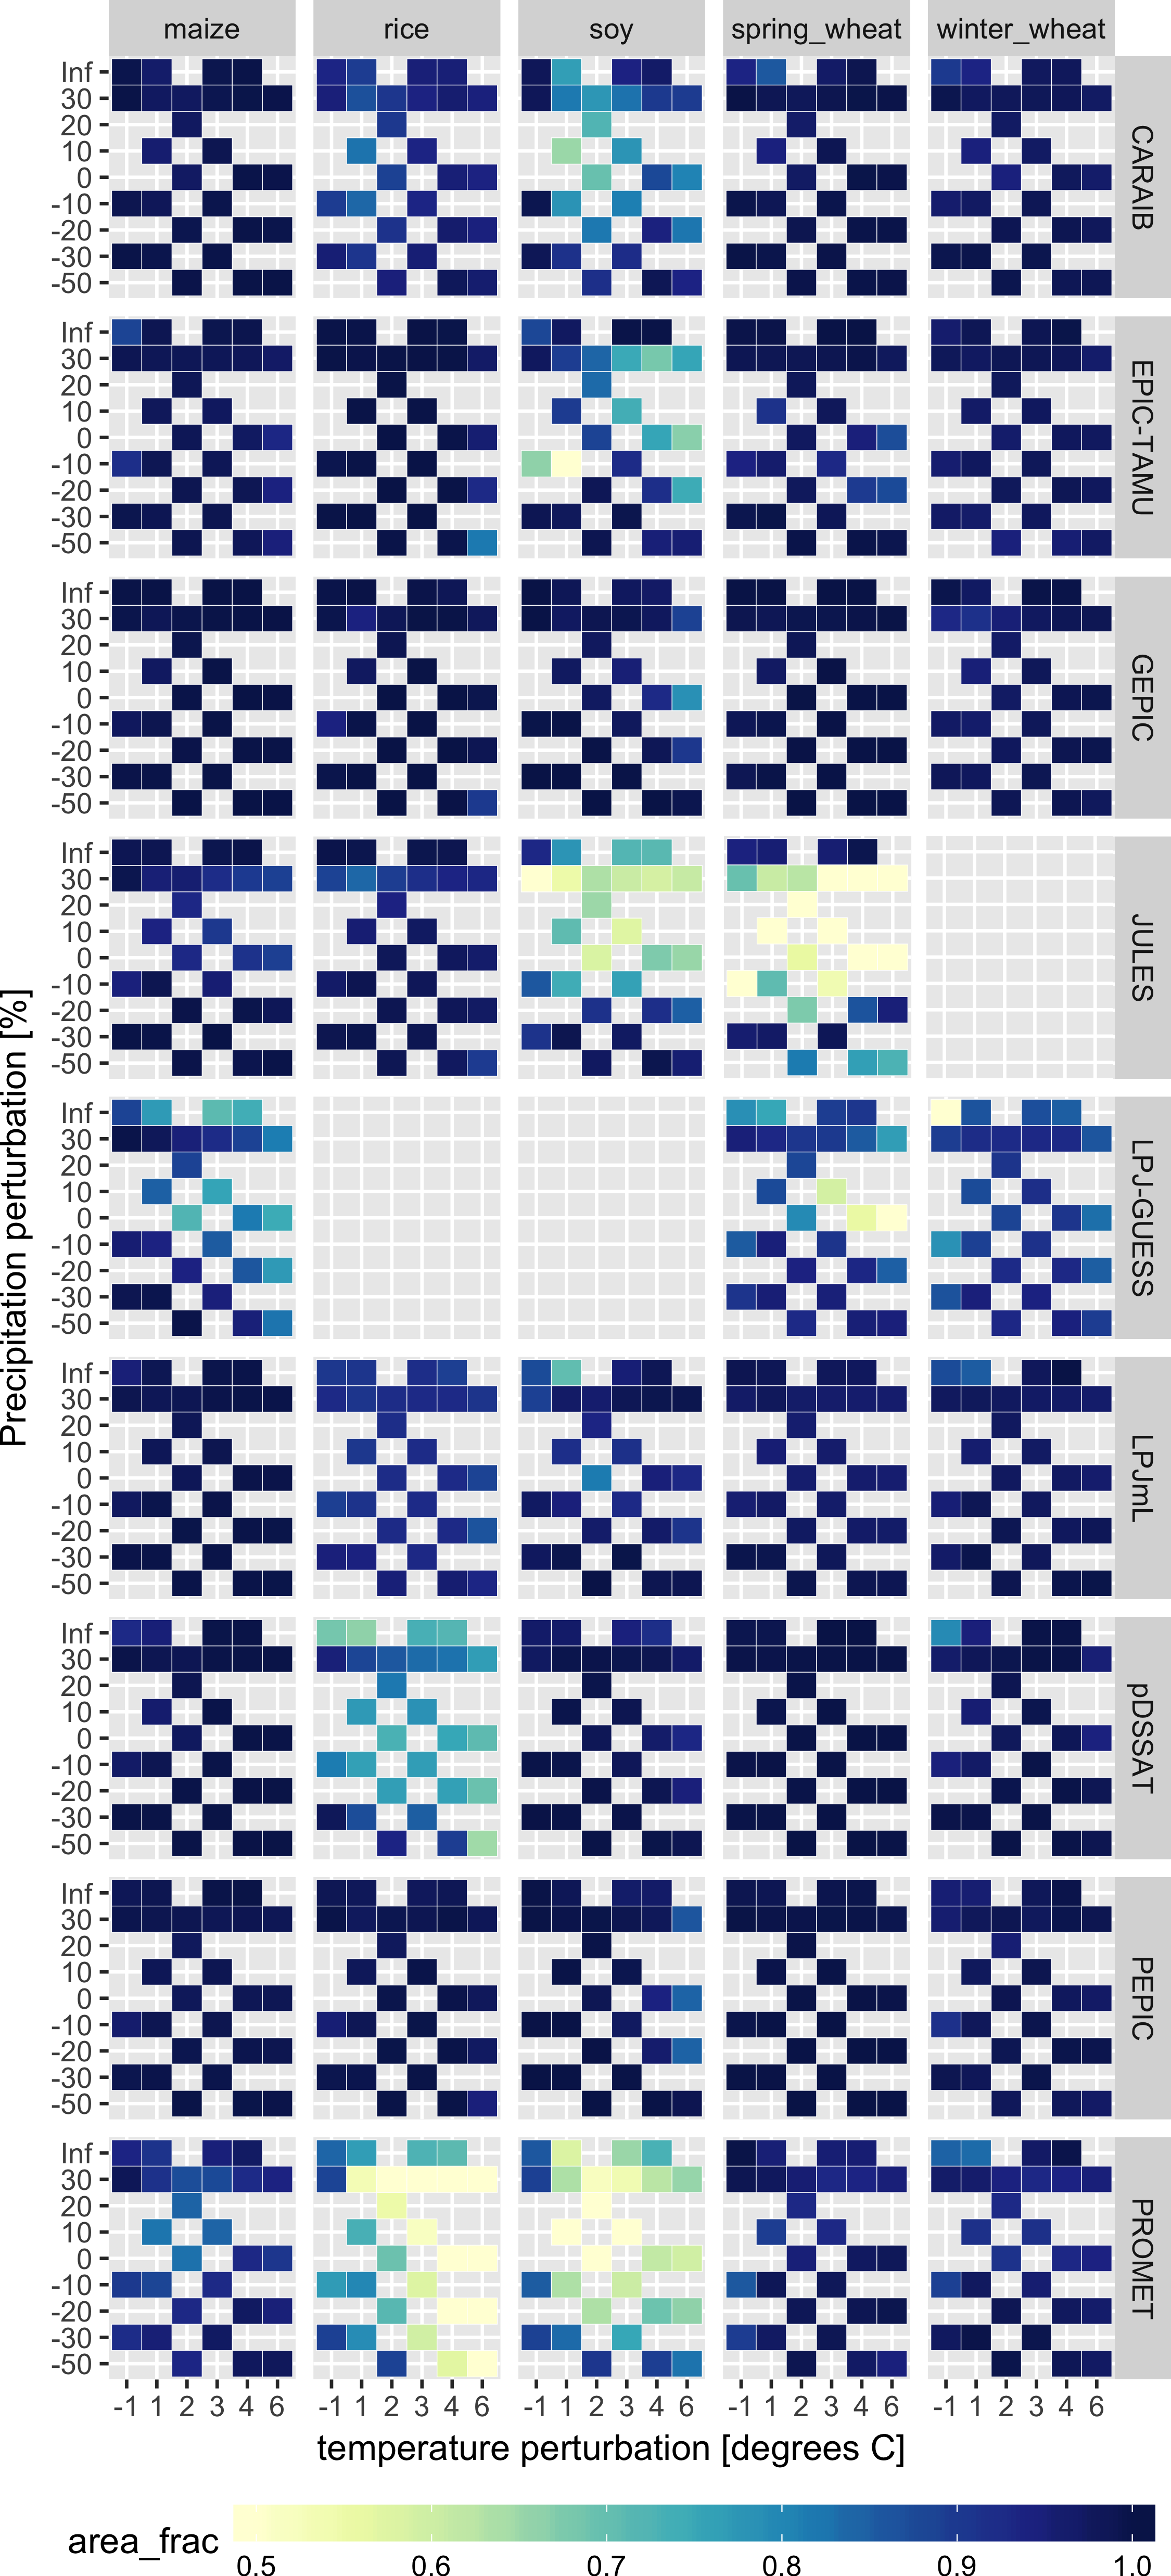
\includegraphics[width=6cm]{figures/error_360.png}
    \caption{Assessment of emulator performance over currently cultivated areas based on normalized error (Equations \ref{eqn:error}, \ref{eqn:per_yield}). 
    We show performance of all 9 models emulated, over all crops and all sampled T and P inputs, but with CO$_2$ and nitrogen held fixed at baseline values. 
    Large columns are crops and large rows models; squares within are T, P scenario pairs. 
    Colors denote the fraction of currently cultivated hectares (``area frac'') for each crop with normalized area $e$ less that 1 indicating the the error between the emulation and simulation less that one standard deviation of the ensemble simulation spread. 
    Of the 63 scenarios at a single CO$_2$ and N value, we consider only those for which all 9 models submitted data (Figure SX) so the model ensemble standard deviation can be calculated uniformly in each case. 
    JULES did not simulate winter wheat and LPJ-GUESS did not simulate rice and soy. Emulator performance is generally satisfactory, with some exceptions. 
    Emulator failures (significant areas of poor performance) occur for individual crop-model combinations, with performance generally degrading for hotter and wetter scenarios.}
   \label{fig:error_360}
\end{figure}

\begin{figure}[ht]
\centering
    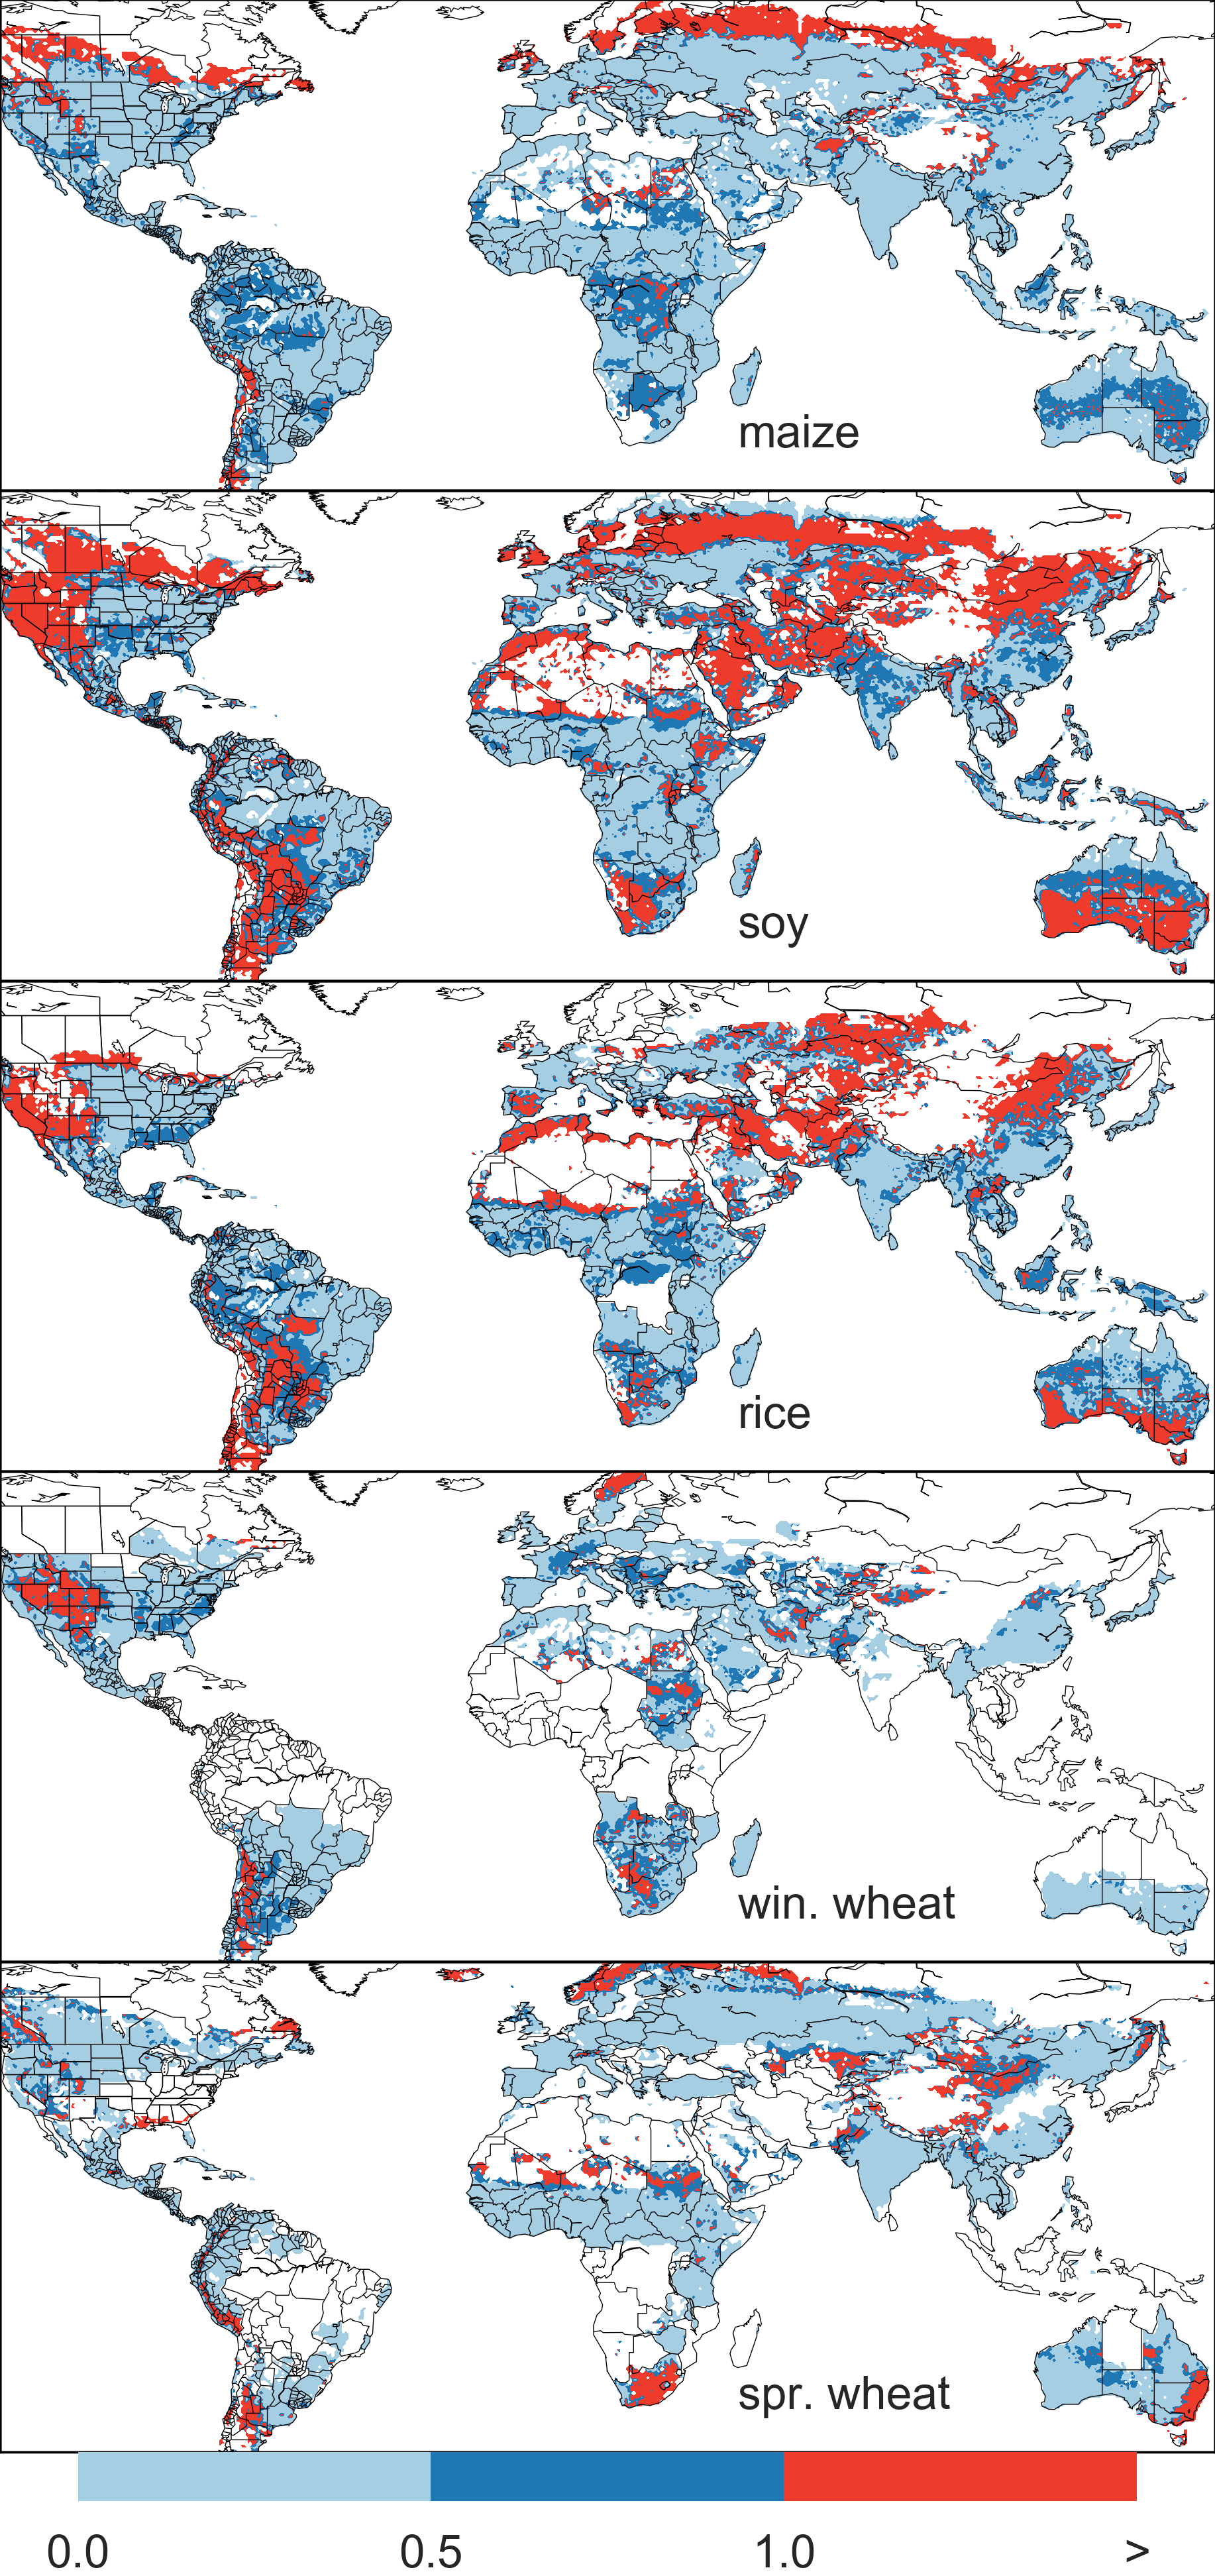
\includegraphics[width=6cm]{figures/em_err.png}
    \caption{Illustration of our test of emulator performance, applied to the CARAIB model for the T+4 scenario for rainfed crops. 
    Contour colors indicate the normalized emulator error $e$, where $e > 1$ means that emulator error exceeds the multi-model standard deviation. 
    White areas are those where crops are not simulated by this model. 
    Models differ in their areas omitted, meaning the number of samples used to calculate the multi-model standard deviation is not spatially consistent in all locations. 
    Emulator performance is generally good relative to model spread in areas where crops are currently cultivated (compare to Figure 1) and in temperate zones in general; emulation issues occur primarily in marginal areas with low yield potentials. 
    For CARAIB, emulation of soy is more problematic, as was also shown in Figure \ref{fig:error_360}.}
   \label{fig:error}
\end{figure}

No general criteria exist for defining an acceptable crop model emulator, so we present two different metrics. 
First, for a multi-model comparison exercise like GGCMI Phase II, one reasonable criterion is what we term the ``normalized error'', which compares the fidelity of an emulator for a given model and scenario to the inter-model uncertainty. 
Second, we show a out-of-sample cross-validation aggregate error for each model independent of the ensemble. 
We define the normalized error $e$ for each scenario as the difference between the fractional yield change from the emulator and that in the original simulation, divided by the standard deviation of the multi-model spread (Equations \ref{eqn:per_yield} and  \ref{eqn:error}):

\begin{equation}
    \label{eqn:per_yield}
    F_{\: scn.}= \frac{Y_{scn.}-Y_{baseline}}{Y_{baseline}}
\end{equation}

\begin{equation}
    \label{eqn:error}
    e_{\: scn.} = \frac{F_{em, \: scn.}-F_{sim, \: scn.}}{\sigma_{sim, \: scn.}}
\end{equation}

Here $F_{\: scn.}$ is the fractional change in a model's mean emulated or simulated yield from the defined historical baseline, in a certain setting or scenario (scn.) in C, T, W, and N space; $Y_{scn.}$ and $Y_{baseline}$ are the absolute emulated or simulated mean yields. 
The normalized error $e$ is the difference between the emulated fractional change in yield and that actually simulated, normalized by $\sigma_{sim}$, the standard deviation in simulated fractional yields change $F_{sim,\: scn.}$ across all models. 
The emulator is fitted across all available simulation outputs for each grid cell, model, and crop, and then the error is calculated across the each of the simulation scenarios provided by all nine models (Figure SX). 

The normalized error metric implies that emulation is generally satisfactory, with several distinct exceptions. 
Almost all model-crop combination emulators have normalized errors less than one over nearly all currently cultivated hectares (Figure \ref{fig:error}), but some individual model-crop combinations are difficult to emulate (e.g.\ PROMET for rice and soy, JULES for soy and spring wheat, Figures SXX-XX). 
Problems with emulating PROMET for rice and soy may have to do with the parametrization of the phenology for those crops which lengthens the growing season in some cases. 
Normalized errors for soy are somewhat higher across all models not because emulator fidelity is worse but because models agree more closely on yield changes for soy than for other crops (see Figure SXX), lowering the denominator. 
Emulator performance often degrades in geographic locations where crops are not currently cultivated. 
For example, emulator performance may be satisfactory over cultivated areas for all crops, but uncultivated regions may show some problematic areas (Figure \ref{fig:error} shows a CARAIB model case, see also Figure SXX).

The normalized error assessment procedure is relatively forgiving for several reasons. 
First, each emulation is evaluated against the simulation actually used to train the  (in-sample validation). 
Had we used a spline interpolation the error would necessarily be zero. 
Second, the performance metric scales emulator fidelity not by the magnitude of yield changes but by the inter-model spread in those changes. 
The normalized error $e$ for a model depends not only on the fidelity of its emulator in reproducing a given simulation but on the particular suite of models considered in the intercomparison exercise. 
Where models differ more widely, the standard for emulators becomes less stringent. 
Ensemble spread dependence can be readily seen when comparing assessments of emulator performance in simulations at baseline CO$_2$ (Figure \ref{fig:error_360}) with those at higher CO$_2$ levels (Figure SXX) because models disagree on the magnitude of CO$_2$ fertilization. 
The rationale for this choice of assessment metric is to relate the fidelity of the emulation to an estimate of true uncertainty, which we take as the multi-model spread. 
We therefore do not provide a formal parameter uncertainty analysis, but note that the GGCMI Phase II dataset is well-suited to statistical exploration of emulation approaches and quantification of emulator fidelity. 
More rigorous emulator assessments that could be preformed in future work include: testing other statistical specifications including non-parametric models and calculating standard error on emulator parameters.

\begin{table*}[t]
\caption{Mean absolute error of emulator representation of a simulation as a percentage of baseline yield for the cross-validation process for rainfed crops. 
A 3-fold stratified k-fold cross validation scheme is utilized where the model is trained on two-thirds of the data and validated on the held-out remaining third (repeated three times). 
The split does not represent a uniform number of samples in each location or in each model because simulation sampling extent in variable space is heterogeneous. 
The calculation only includes grid cells with at least 1\% of surface area cultivated with a specific crop (approximately 1000 grid cells in each case). 
The table shows the mean error (`WM') weighted by hectares grown in each grid cell \citep{Portmann2010} and the unweighted median across included grid cells `MD'. 
* Indicates cases where the OLS linear model fails.} 
\label{table:ASE}
\begin{tabular}{l | cc | cc | cc | cc | cc} 
\hline
{} & \multicolumn{2}{c|}{\textbf{Maize}} & \multicolumn{2}{c|}{\textbf{Soy}}& \multicolumn{2}{c |}{\textbf{Rice}} & \multicolumn{2}{c |}{\textbf{S. Wheat}} & \multicolumn{2}{c}{\textbf{W. Wheat}} \\
\textbf{Model}     & WM (\%)& MD (\%)& WM (\%)& MD (\%)& WM (\%)& MD (\%)& WM (\%)& MD (\%)& WM (\%) & MD (\%) \\ \hline
\textbf{CARAIB}    & 0.00  & 1.71  & 0.02  & 2.39  & 0.03  & 2.95  & 0.02  & 4.40  & 0.01  & 2.36  \\ \hline
\textbf{EPIC-TAMU} & 0.00  & 4.30  & 0.01  & 6.24  & 0.00  & 3.35  & 0.01* & 6.82* & 0.01  & 3.51  \\ \hline
\textbf{JULES}     & 0.11  & 6.13  & 0.01  & 10.2  & 0.01  & 6.97  & 0.04  & 15.1  & NA    & NA    \\ \hline
\textbf{GEPIC}     & 0.00  & 5.78  & 0.00  & 3.75  & 0.01  & 5.64  & 0.01  & 6.76  & 0.01  & 7.01  \\ \hline
\textbf{LPJ-GUESS} & 0.00  & 1.78  & NA    & NA    & NA    & NA    & 0.05  & 6.22  & 0.02  & 3.35  \\ \hline
\textbf{LPJmL}     & 0.00  & 9.44  & 0.00  & 3.25  & 0.01  & 8.37  & 0.01  & 9.83  & 0.01  & 4.98  \\ \hline
\textbf{pDSSAT}    & 0.00  & 2.93  & 0.05  & 3.02  & 0.01  & 3.97  & 0.01  & 2.97  & 0.01  & 4.67  \\ \hline
\textbf{PROMET}    & 0.01  & 4.19  & 0.00  & 6.03  & 0.01  & 9.85  & 0.01  & 7.04  & 0.01  & 3.68   \\ \hline
\textbf{PEPIC}     & 0.00* & 3.71* & 0.00* & 2.80* & 0.00* & 2.89* & 0.00* & 4.83* & 0.02* & 6.70*  \\ \hline
\end{tabular}
\end{table*}

We also provide a more stringent test of emulator performance; a three-fold cross validation (out-of-sample validation). 
Here the training data is split and the model is trained on two thirds of the data and tested on the held out portion (the process is then repeated three times to cover all data in the training set). 
We normalize the error in each grid cell by dividing by the yield in that grid cell in the baseline (T+0, W+0, C=360, N=200) case and show aggregations by grid cell and weighted by area cultivated per grid cell. 
Errors are generally low as a percentage of yield --even for this strict protocol-- and when weighted by area, essentially zero in most cases (Table \ref{table:ASE}). 
Note that the cross validation process often does not include ``edge'' simulations in the training set (i.e. those at the highest or lowest value in that dimension) on one or more folds of the training set split.
The ``edge'' cases are then predicted during the prediction phase of cross validation.
Such an extrapolation during cross validation is not representative based on the intended use of the emulator, which should only be used within the sample space of the overall training set.

%%%%%%%%%%%%%%%%%%%%%%%%%%%%%%%%%%%%%%%%%%%%%%%%%%%%%%%%%%%%%%%
%%%%%%%%%%%%%%%%%%%%%%%%%%%%%%%%%%%%%%%%%%%%%%%%%%%%%%%%%%%%%%%
%%%%%%%%%%%%%%%%%%%%%%%%%%%%%%%%%%%%%%%%%%%%%%%%%%%%%%%%%%%%%%%
\section{Emulator results and products}
\label{S:5}
\begin{figure*}[ht]
  \centering
  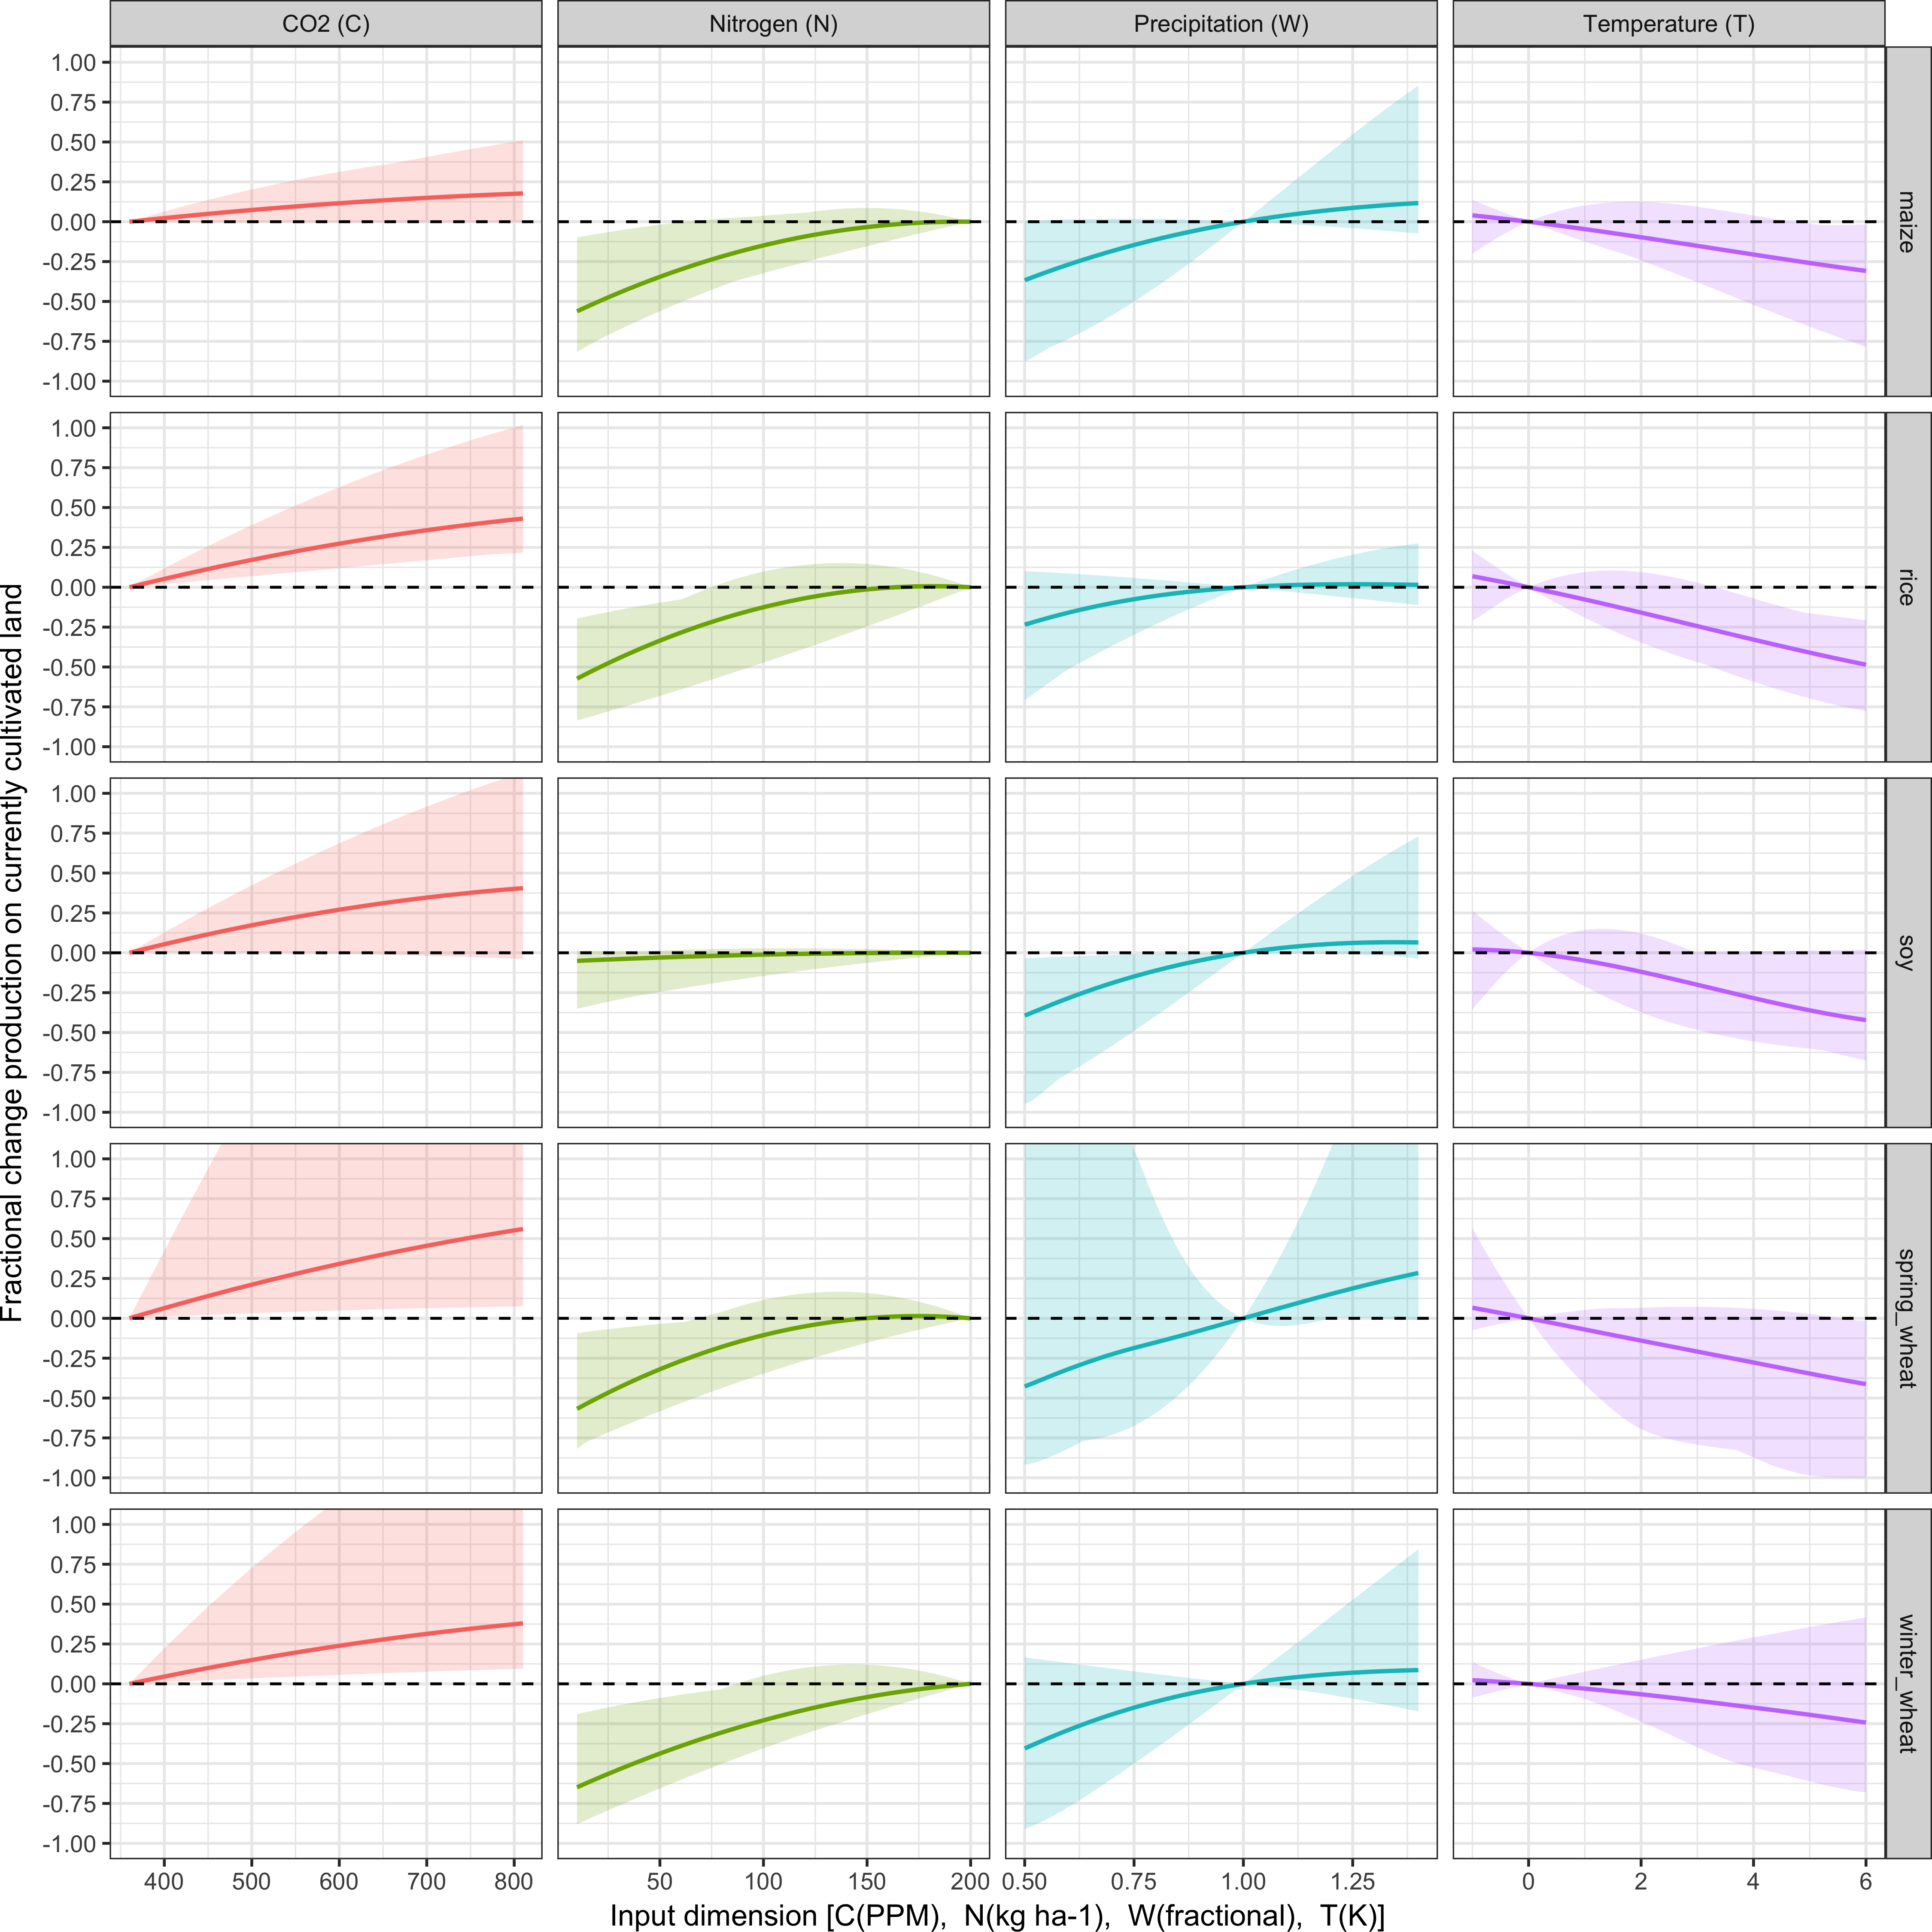
\includegraphics[width = 15cm]{figures/em_CTWN_all_crops.png}
  \caption{Emulated global damage functions for the five crops included in GGCMI Phase II, from the multi-model mean, for the four dimensions varied: CO$_2$, temperature, water, and nitrogen (collectively ``CTWN''). 
  Solid line shows the multi-model ensemble median and shaded area shows the high and low model projection. 
  All other covariates held constant at baseline values (T+0K, W+0\%, C = 360ppm, and N = 200kg ha-1). 
  Damages are reported as fractional change in production relative to the baseline case over currently cultivated land \citep{Portmann2010}.
  }
  \label{fig:all_dims}
\end{figure*}

\begin{figure}[ht]
    \centering
    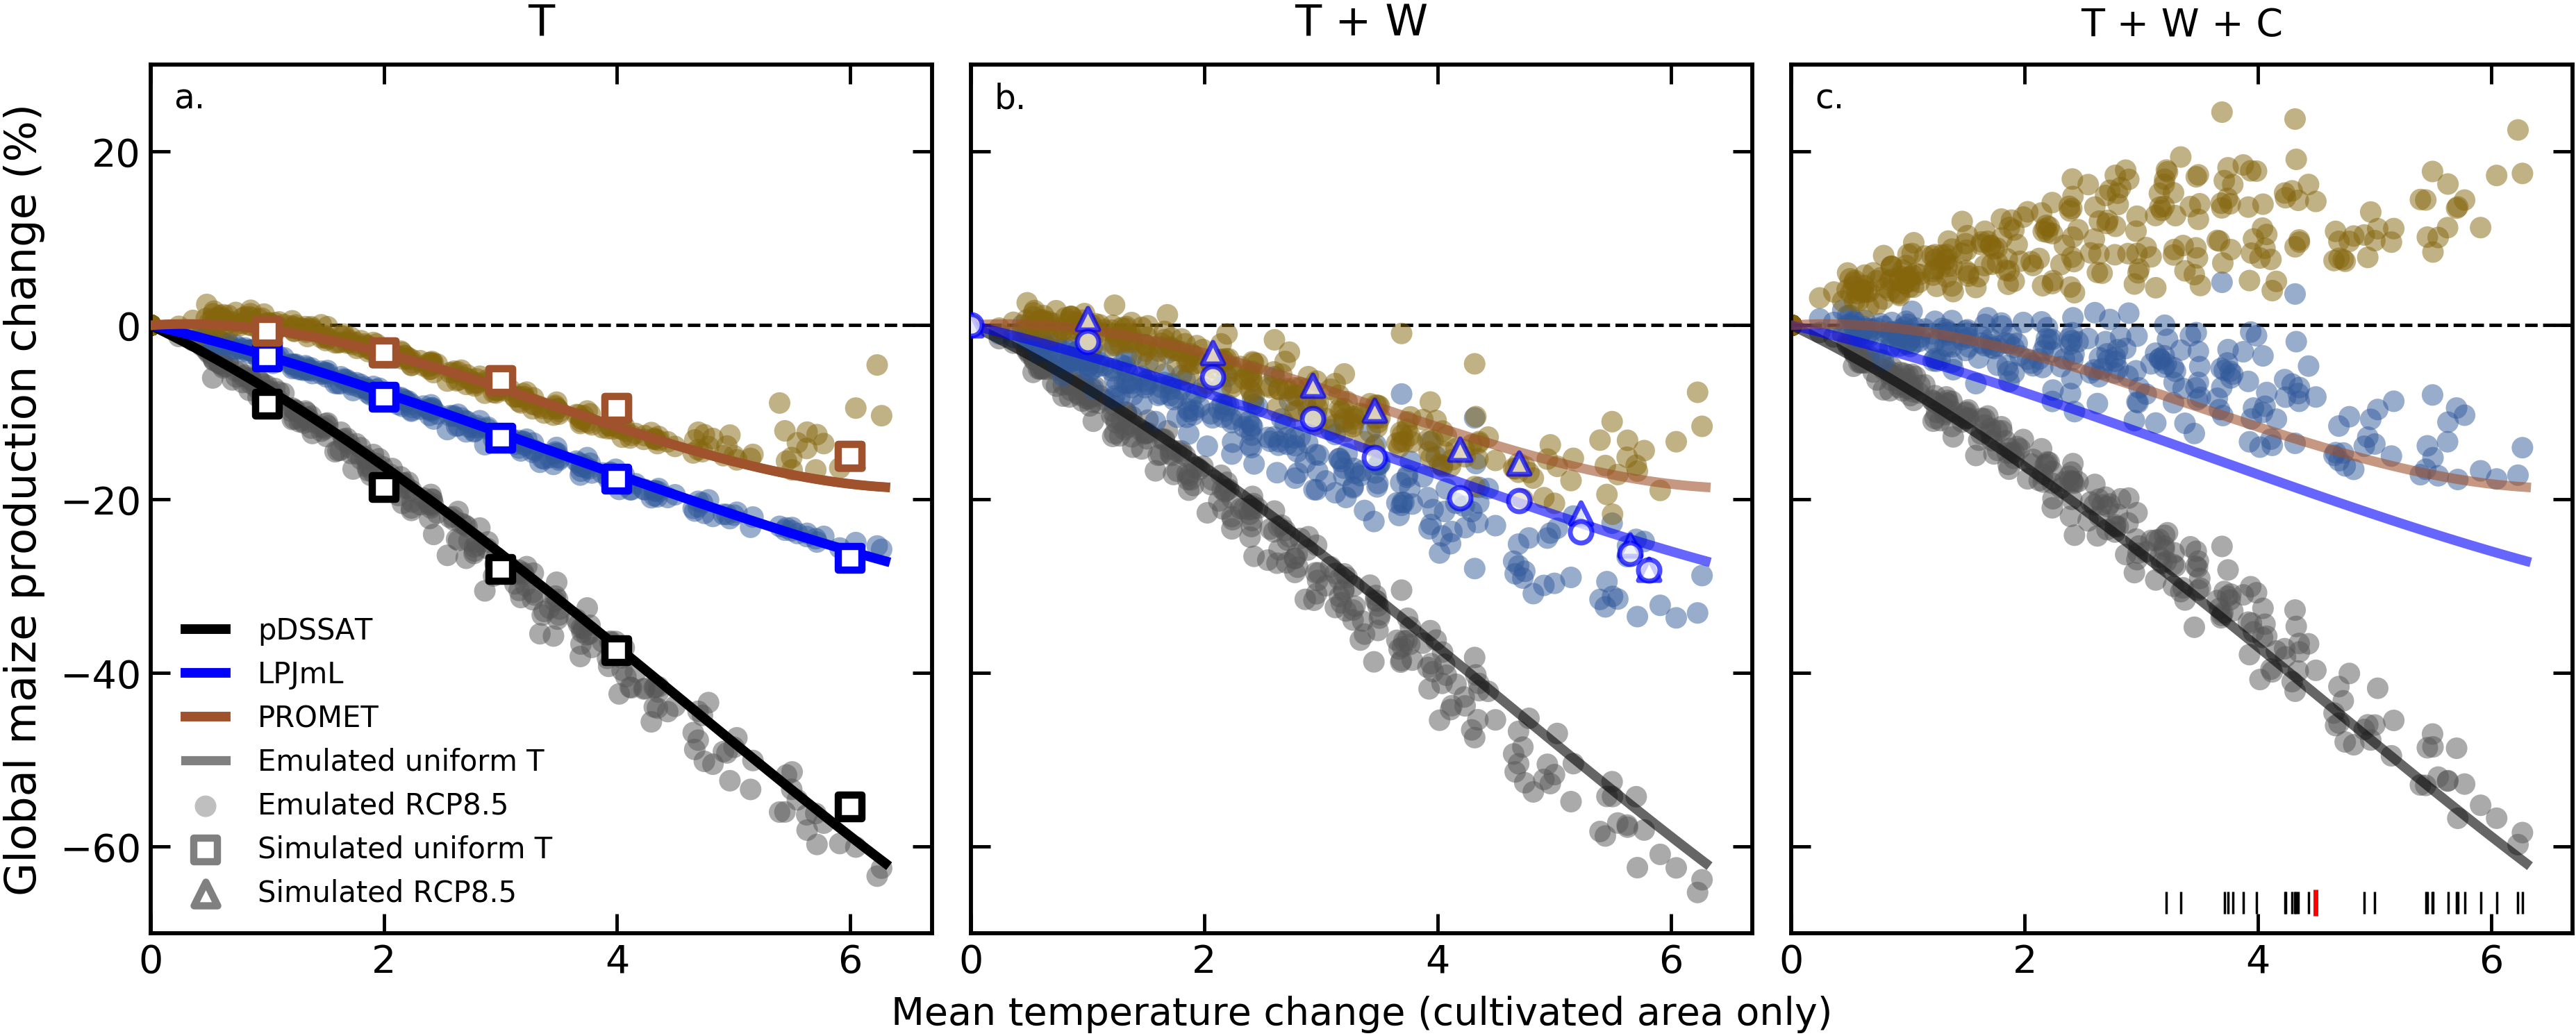
\includegraphics[width = 8.3cm]{figures/global_em_maize.png}
    \caption{Global emulated damages for maize on currently cultivated lands for three example GGCMI Phase II models. 
    Models not shown: CARAIB, EPIC-TAMU, JULES, GEPIC, LPJ-GUESS, and PEPIC.
    Scatter points show the emulated production change from the 1980-2010 mean value for each crop model using inputs from 30 climate models from the CMIP-5 archive \citep{Taylor2012} at the decadal timescale for RCP 8.5.
    The x-axis represents the mean temperature shift over all grid cells where crops are grown (unweighted).
    Temperature and precipitation vary in the climate runs but the effects of CO$_2$ are not included here.
    Open square markers show the Phase II simulated values at each temperature level with other inputs held at baseline values (W+0\%, C = 360ppm, and N = 200kg ha-1).
    Bold lines show emulated values with uniform global temperature shifts applied and precipitation held constant. 
    Rug plots show end of century (2090-2100 mean) values for temperature change for each CMIP-5 model and resultant production change for each crop and climate model combination (including the six models not shown in full).
    In all cases nitrogen is fixed at 200 (kg ha$^-1$) and global production values are aggregated up from the grid cell level based on the growing areas for rainfed and irrigated maize \citep{Portmann2010}. 
    }
    \label{fig:globe_em}
\end{figure}

\begin{figure}[ht]
\centering
   \includegraphics[width=7cm]{figures/figure_10_alt_1.png} \hspace{10mm} \includegraphics[width=7cm]{figures/figure_10_alt_2.png}
   \caption{alternate
   }
   \label{fig:yearly}
\end{figure}

Because the emulator or ``surrogate model'' transforms the discrete simulation sample space into a continuous response surface at any geographic scale, it can be used for a variety of applications, including construction of continuous damage functions. 
As an example, we present global damage functions constructed from the 4D emulation, across all four dimensions tested in this study (Figure \ref{fig:all_dims}). 
In general, across model spread is qualitatively similar across different crops and different dimensions with some notable exceptions. 
Model spread is highest for spring wheat in general and the CO$_2$ response for the wheats and soy.
On the other side, muted responses include soy, an efficient atmospheric nitrogen-fixer, is relatively insensitive to nitrogen, rice is not generally grown in water-limited conditions so it shows the lowest response to changes in precipitation, and maize has a muted response to CO$_2$ as a C4 plant.

Note that these functions are presented only as examples and do not represent true global projections, because they are developed from simulation data with a uniform temperature shift while increases in global mean temperature should manifest non-uniformly in space and distributions \citep[e.g]{Sippel2015}. 
The global coverage of the GGCMI Phase II simulations allows impacts modelers to apply arbitrary geographically-varying climate projections, as well as arbitrary aggregation masks, to develop damage functions for any climate scenario and any geopolitical or geographic level bigger than 0.5 degrees in latitude and longitude.

Finally, the emulator can be used to quickly project crop yield responses to climate change under a variety of conditions. 
The emulated crop model yield responses to business-as-usual climate change (Representative Concentration Pathway (RCP) 8.5) are shown in Figure \ref{fig:globe_em}.

30 climate models from the CMIP-5 archive \citep{Taylor2012}. 


aggregated to global yield, \textcolor{red}{with simulated transient climate run values shown for comparison} (Figure \ref{fig:globe_em}, which shows maize on currently cultivated land). 


%%%%%%%%%%%%%%%%%%%%%%%%%%%%%%%%%%%%%%%%%%%%%%%%%%%%%%%%%%%%%%%
%%%%%%%%%%%%%%%%%%%%%%%%%%%%%%%%%%%%%%%%%%%%%%%%%%%%%%%%%%%%%%%
%%%%%%%%%%%%%%%%%%%%%%%%%%%%%%%%%%%%%%%%%%%%%%%%%%%%%%%%%%%%%%%

\section{Discussion and conclusions} 
\label{S:6}
We show that the systematic parameter sampling in the GGCMI Phase II experiments allow emulating climatological crop yield responses with a relatively simple reduced-form statistical model. 
The sampling provides information on the influence of multiple interacting factors in a way that realistic climate model simulations cannot, and allows isolating long-term impacts from confounding factors that lead to different year-over-year responses. 
The use of a relatively simple functional form in turn offers the possibility of physical interpretation of parameter values that can assist in model intercomparison and evaluation. 
The yield output for a single GGCMI Phase II model that simulates all scenarios and all five crops is $\sim$12.5 GB; the emulator is $\sim$20 MB, a reduction of nearly three orders of magnitude. 

Several cautions should be noted when using the emulator. While the emulator allows estimating agricultural impacts under arbitrary climate scenarios, extrapolation outside the sample space should be avoided. 
Additionally, because the simulation protocol was designed to focus on change in yield under climate perturbations and not on replicating real-world yields, the models are not formally calibrated so cannot be used for impacts projections except in conjunction with historical yield information. 
Finally, because the GGCMI Phase II simulations apply uniform perturbations to historical climate inputs, they do not sample potential changes in climate variability. 
Although such changes are uncertain and remain poorly characterized \citep[e.g.][]{Alexande2006, Kodra2014}, follow-up experiments may wish to consider them. 
Several recent studies have described procedures for generating simulations that combine historical data with model projections of changes in the marginal distributions or temporal dependence of temperature and precipitation(e.g.\ \citet{Leeds2015, poppick2016, Won16} and \citet{Haugen2018}).

The GGCMI Phase II dataset invites a broad range of potential future avenues of analysis, especially because emulation allows statistical distillation of the large dataset (40 billion simulated yields) into a tractable form. 
Potential studies might include a detailed examination of interaction terms between the major input drivers, robust quantification of model sensitivities to input drivers, exploration of yield responses to extremes, and evaluation of geographic shifts in optimal growing regions. 
The dataset also enables studies of emulation itself, including a more systematic evaluation of different statistical and machine learning model specifications.
In general, the development of multi-model ensembles involving systematic parameters sweeps has large promise for better understanding potential future crop responses and for improving process-based crop models.

%%%%%%%%%%%%%%%%%%%%%%%%%%%%%%%%%%%%%%%%%%%%%%%%%%%%%%%%%%%%%%%
\codedataavailability{The polynomial emulator parameter matrices for all crop model emulators are available at {doi.org/10.5281/ zenodo.2605374.}}

%\appendix
%\section{}
%\subsection{Data Access}
%\noappendix %% use this to mark the end of the appendix section

\authorcontribution{J.E., C.M, A.R., J.F., and E.M.\ designed the research. C.M., J.J., J.B., P.C., M.D., P.F., C.F., L.F., M.H., C.I., I.J., C.J., N.K., M.K., W.L., S.O., M.P., T.P., A.R., X.W., K.W., and F.Z.\ performed the simulations. J.F., J.J., A.S., M.L., and E.M.\ performed the analysis and J.F., C.M., and E.M.\ prepared the manuscript.}

\competinginterests{The authors declare no competing interests.}

\begin{acknowledgements}
We thank Michael Stein and Kevin Schwarzwald, who provided helpful suggestions that contributed to this work. 
This research was performed as part of the Center for Robust Decision-Making on Climate and Energy Policy (RDCEP) at the University of Chicago, and was supported through a variety of sources. 
RDCEP is funded by NSF grant \#SES-1463644 through the Decision Making Under Uncertainty program. J.F.\ was supported by the NSF NRT program, grant \#DGE-1735359. 
C.M.\ was supported by the MACMIT project (01LN1317A) funded through the German Federal Ministry of Education and Research (BMBF). 
C.F.\ was supported by the European Research Council Synergy grant \#ERC-2013-SynG-610028 Imbalance-P. 
P.F.\ and K.W.\ were supported  by the Newton Fund through the Met Office Climate Science for Service Partnership Brazil (CSSP Brazil). 
K.W.\ was supported by the IMPREX research project supported by the European Commission under the Horizon 2020 Framework programme, grant \#641811. 
A.S.\ was supported by the Office of Science of the U.S. Department of Energy as part of the Multi-sector Dynamics Research Program Area. 
S.O.\ acknowledges support from the Swedish strong research areas BECC and MERGE together with support from LUCCI (Lund University Centre for studies of Carbon Cycle and Climate Interactions). 
R.C.I.\ acknowledges support from the Texas Agrilife Research and Extension, Texas A \& M University. 
This is paper number 35 of the Birmingham Institute of Forest Research. 
Computing resources were provided by the University of Chicago Research Computing Center (RCC).
\end{acknowledgements}

\bibliographystyle{copernicus}
\bibliography{bib}

\end{document}

%%%%%%%%%%%%%%%%%%%%%%%%%%%%%%%%%%%%%%%%%%%%%%%%%%%%%%%%%%%%%%%
%%%%%%%%%%%%%%%%%%%%%%%%%%%%%%%%%%%%%%%%%%%%%%%%%%%%%%%%%%%%%%%
%%%%%%%%%%%%%%%%%%%%%%%%%%%%%%%%%%%%%%%%%%%%%%%%%%%%%%%%%%%%%%%
%%%%%%%%%%%%%%%%%%%%%%%%%%%%%%%%%%%%%%%%%%%%%%%%%%%%%%%%%%%%%%%
%  OLD UNUSED 
%%%%%%%%%%%%%%%%%%%%%%%%%%%%%%%%%%%%%%%%%%%%%%%%%%%%%%%%%%%%%%%
%%%%%%%%%%%%%%%%%%%%%%%%%%%%%%%%%%%%%%%%%%%%%%%%%%%%%%%%%%%%%%%
%%%%%%%%%%%%%%%%%%%%%%%%%%%%%%%%%%%%%%%%%%%%%%%%%%%%%%%%%%%%%%%
%%%%%%%%%%%%%%%%%%%%%%%%%%%%%%%%%%%%%%%%%%%%%%%%%%%%%%%%%%%%%%%


\begin{figure*}[ht]
\centering
    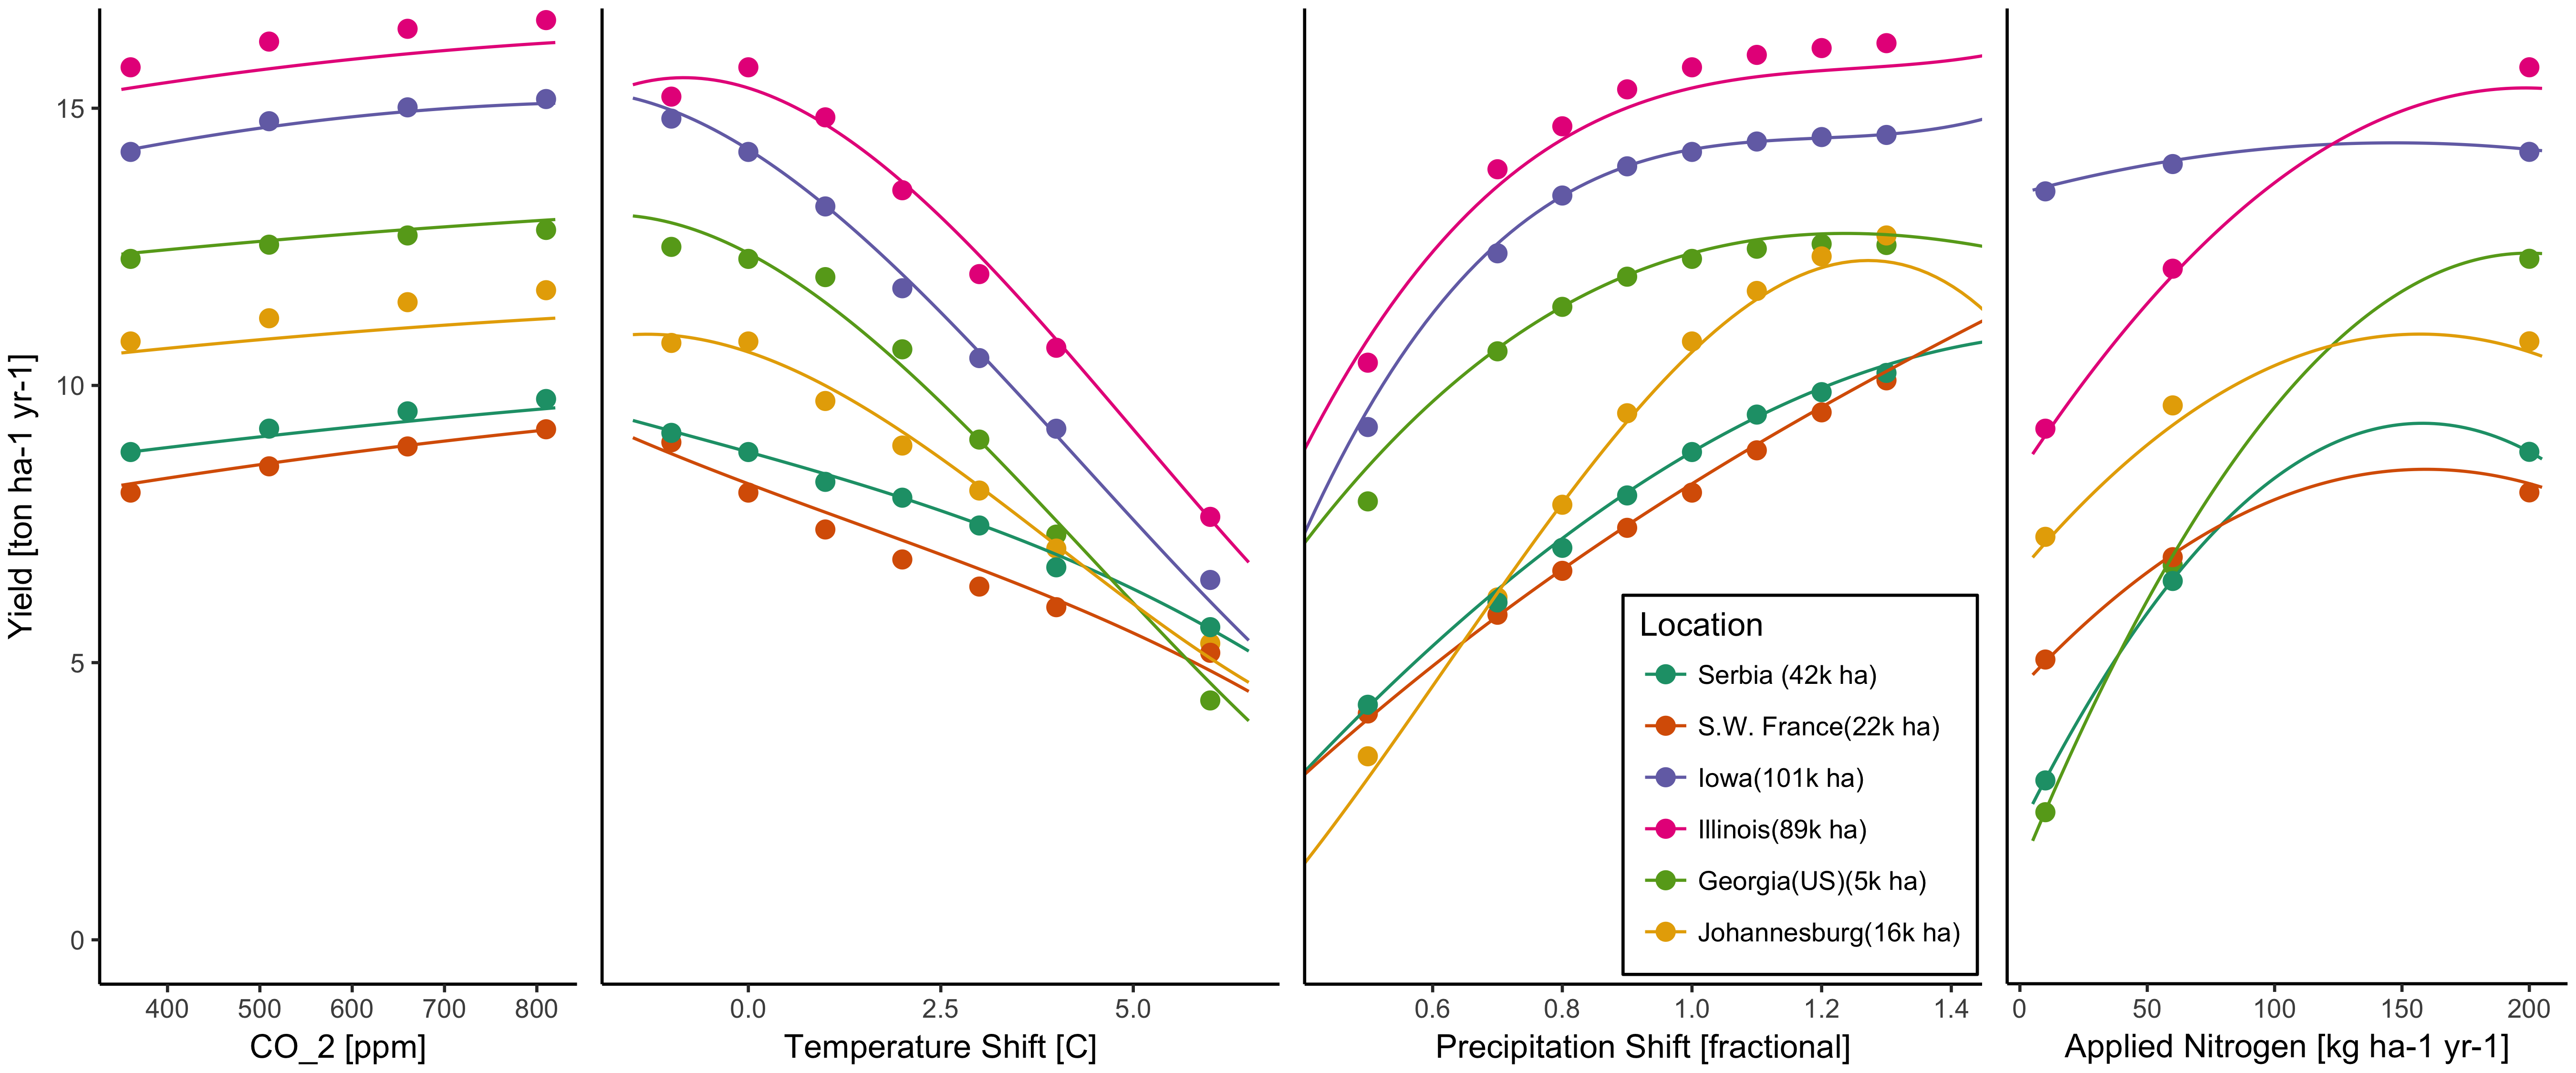
\includegraphics[width=16cm]{figures/regression_areas.png}
    \caption{Illustration of spatial variations in yield response successfully captured by the emulator. 
    We show rainfed maize in the pDSSAT model in six example locations selected to represent high-cultivation areas around the globe. 
    Legend includes hectares cultivated in each selected grid cell. 
    Each panel shows variation along a single variable, with others held at baseline values. 
    Dots show climatological mean yields and lines the results of the full 4D emulator of Equation \ref{eqn:features_original}. 
    In general the climatological response surface is sufficiently smooth that it can be represented within the sampled variable space by the simple polynomial used in this work. 
    Extrapolation can however produce misleading results. 
    Nitrogen fits in some cases may not be realistic at intermediate values given limited sampling. 
    For more detailed emulator assessment, see Appendix B.}
   \label{fig:regression}
\end{figure*}

\begin{figure*}[ht]
\centering
    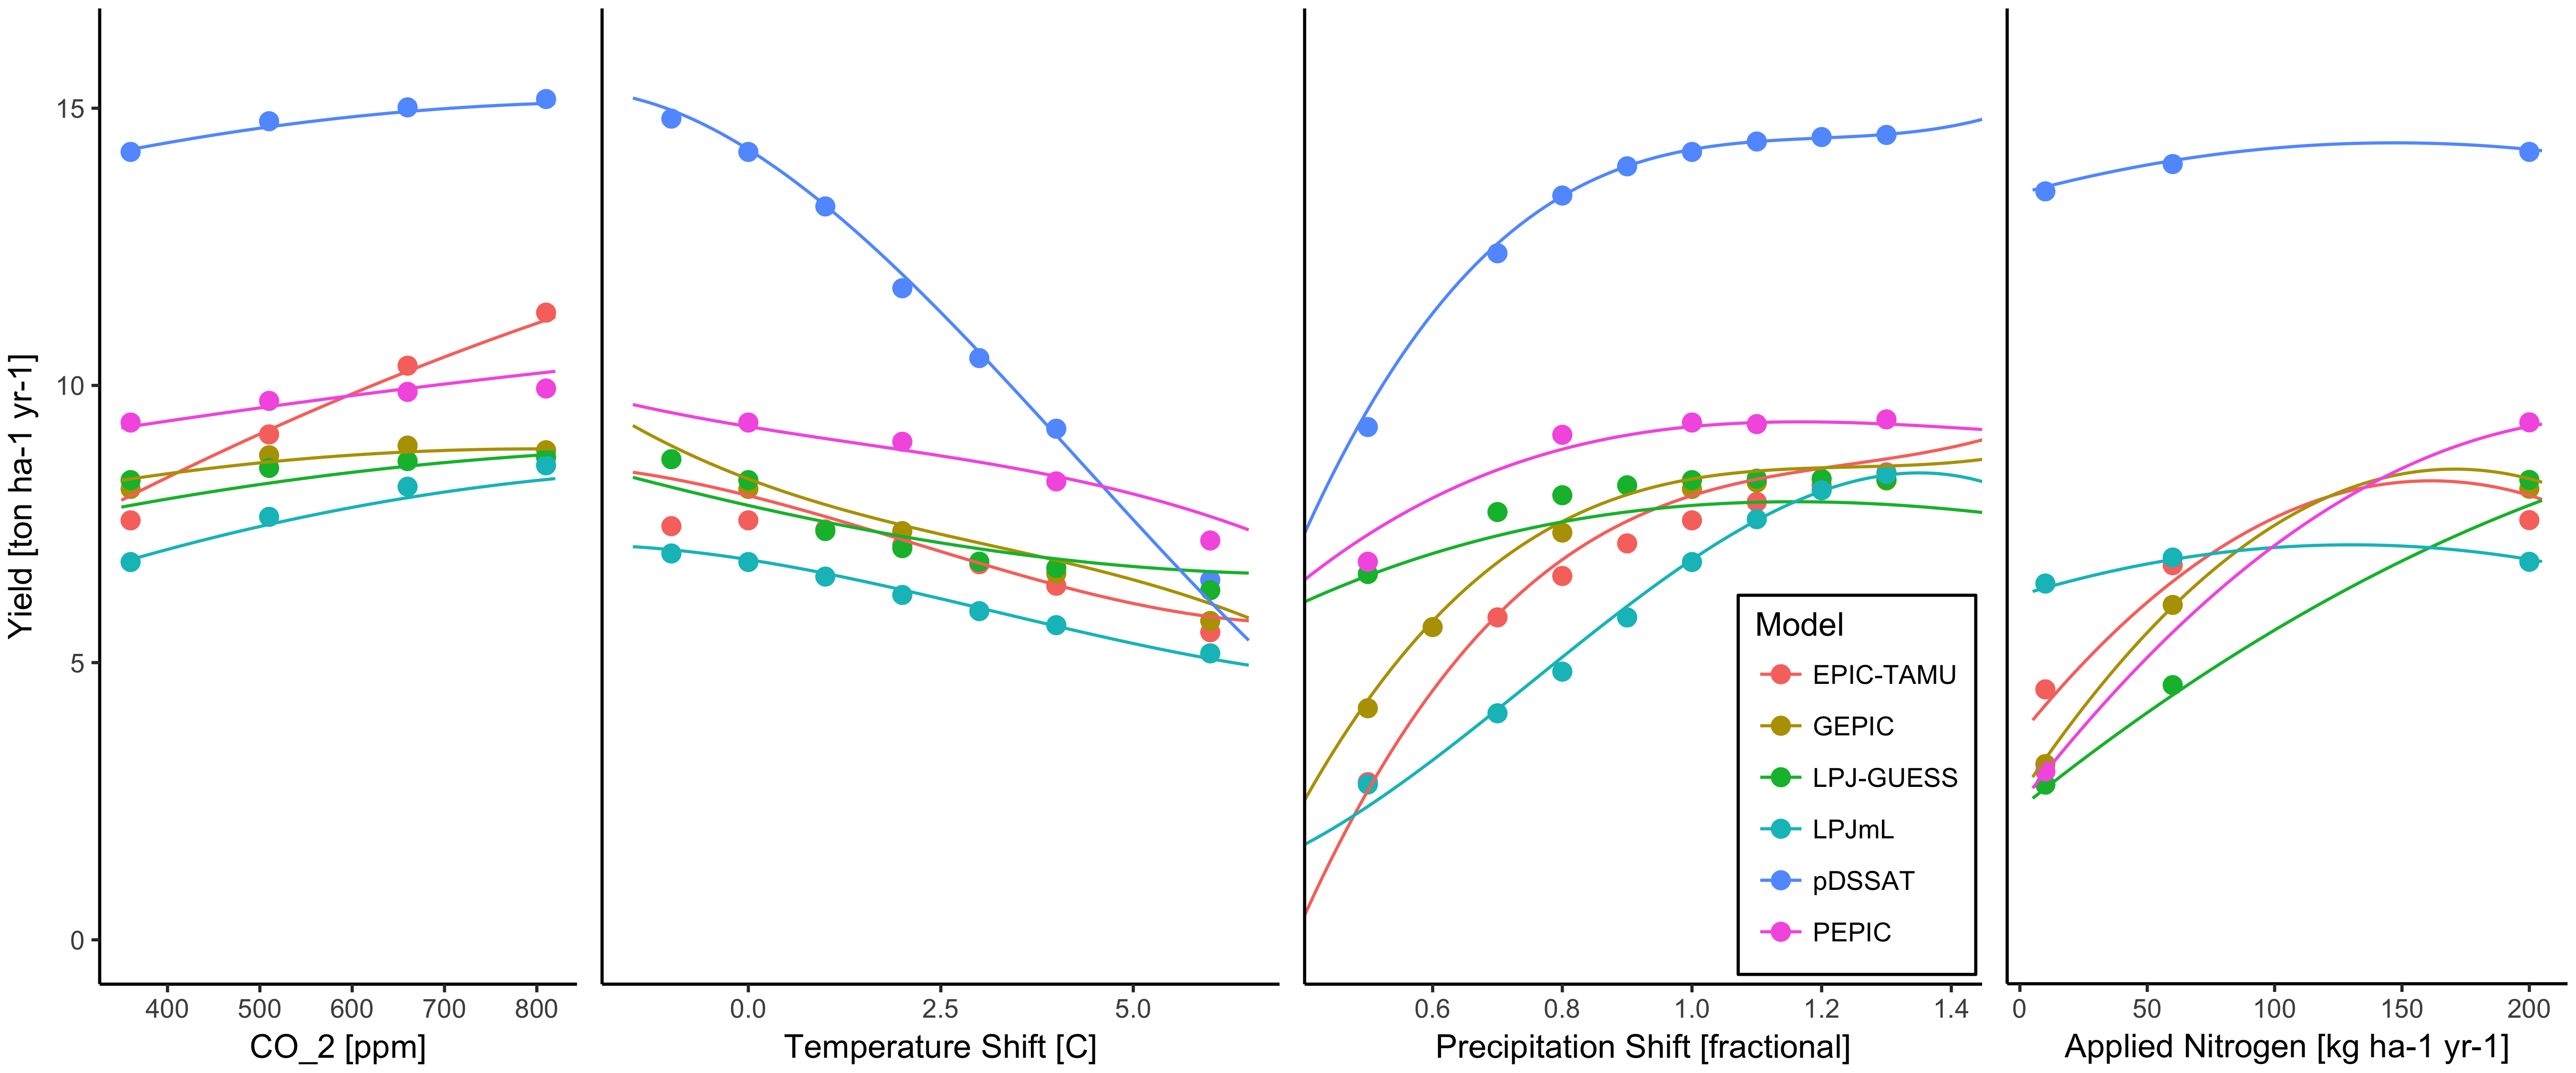
\includegraphics[width=16cm]{figures/regression_model.png}
    \caption{Illustration of across-model variations in yield response successfully captured by the emulator. 
    Figures shows simulations and emulations from six models for rainfed maize in the same Iowa grid cell shown in Figure \ref{fig:regression}, with the same plot conventions. 
    Models that do not simulate the nitrogen dimension are omitted for clarity. 
    Note that models are uncalibrated, increasing spread in absolute yields. 
    While most model responses can readily emulated with a simple polynomial, some response surfaces diverge slightly from the polynomial approach (e.g.\ LPJ-GUESS here) and lead to emulation error, though error generally remains small relative to inter-model uncertainty. 
    For more detailed emulator assessment, see Appendix B. 
    As in Figure \ref{fig:regression}, extrapolation out of the sample space is potentially problematic.}
   \label{fig:regression_iowa}
\end{figure*}

\begin{figure}[ht]
\centering
   \caption{Example showing distinction between crop yield responses to year-to-year and climatological mean precipitation shifts. 
   Figure shows rainfed maize for a representative high-yield region (nine adjacent grid cells in northern Iowa) from the pDSSAT model, for the baseline 1981-2010 historical climate (gray) and for the scenario of maximum and minimum precipitation change (brown and green). 
   Other covariates are held at baseline values.
   Open black circles mark climatological mean yield values for all seven precipitation scenarios (W -50\%, -30\%, -20\%, -10\%, W, +10\%, +20\%, +30\%). 
   Colored lines show total least squares linear regressions of year-over-year variations in each scenario. 
   Bold Black line shows the emulator fit through the climatological mean values.}
   \label{fig:yearvclimpr}
\end{figure}

    {Totals} & {9} & {8} & {8} & {8} & {9} & {8} & {5240 | 3378}\\


We include interaction terms (both linear and higher-order) because past studies have shown them to be significant effects. 
To limit over-fitting and unstable parameter estimation, we apply a feature selection procedure (described below) that reduces the potential 34-term polynomial (for the rainfed case) to 23 terms.
We regress 30-year climatological mean yields against a third-order polynomial in C, T, W, and N with interaction terms. 


\begin{align}
    \label{eqn:features_original}
    Y\ = \ & K_{1}  \\
    + \ & K_{2} C      + K_{3} T      + K_{4} W      + K_{5} N   \nonumber \\
    + \ & K_{6} C^2    + K_{7} T^2    + K_{8} W^2    + K_{9} N^2 \nonumber \\
    + \ & K_{10} C W   + K_{11} C N   + K_{12} T W   + K_{13} T N   + K_{14} W N \nonumber \\
    + \ & K_{15} C T   + K_{16} T^3   + K_{17} W^3   + K_{18} C^3   + K_{19} N^3 \nonumber \\
    + \ & K_{20} T W N + K_{21} T^2 W + K_{22} W^2 T + K_{23} W^2 N + K_{24} C W N \nonumber \\
    + \ & K_{25} C T N + K_{26} N^2 C + K_{27} N^2 T + K_{28} N^2 W + K_{29} T^2 N \nonumber \\
    + \ & K_{30} T^2 C + K_{31} W^2 C + K_{32} C^2 W + K_{33} C^2 T + K_{34} C^2 N \nonumber
\end{align}


%The resulting statistical model (Equation \ref{eqn:features_final}) is used for all grid cells, models, and rainfed crops. 
%(The regressions for irrigated crops do not contain the W terms and the models that do not sample the nitrogen levels omit the N terms.)

%\begin{align}
%    \label{eqn:features_final}
%    Y\ = \ & K_{1}  \\
%       + \ & K_{2}  C     + K_{3}  T     + K_{4}  W     + K_{5}  N   \nonumber \\
%       + \ & K_{6}  C^2   + K_{7}  T^2   + K_{8}  W^2   + K_{9}  N^2 \nonumber \\
%       + \ & K_{10} C W   + K_{11} C N   + K_{12} T W   + K_{13} T N + K_{14} W N \nonumber \\ % lost 1 term, CT
%%      + \ & K_{15} T^3   + K_{16} W^3   + K_{17} T W N  \nonumber \\ % lost 2 terms, C^3 and N^3
%       + \ & K_{18} T^2 W + K_{19} W^2 T + K_{20} W^2 N  \nonumber \\ % lost 2 terms, CWN and CTN
%%      + \ & K_{21} N^2 C + K_{22} N^2 T + K_{23} N^2 W  \nonumber    % lose 6 terms: T^2N and T^2C, W^2C, 3 C^2 terms
%\end{align}


\begin{figure}[ht]
\centering
   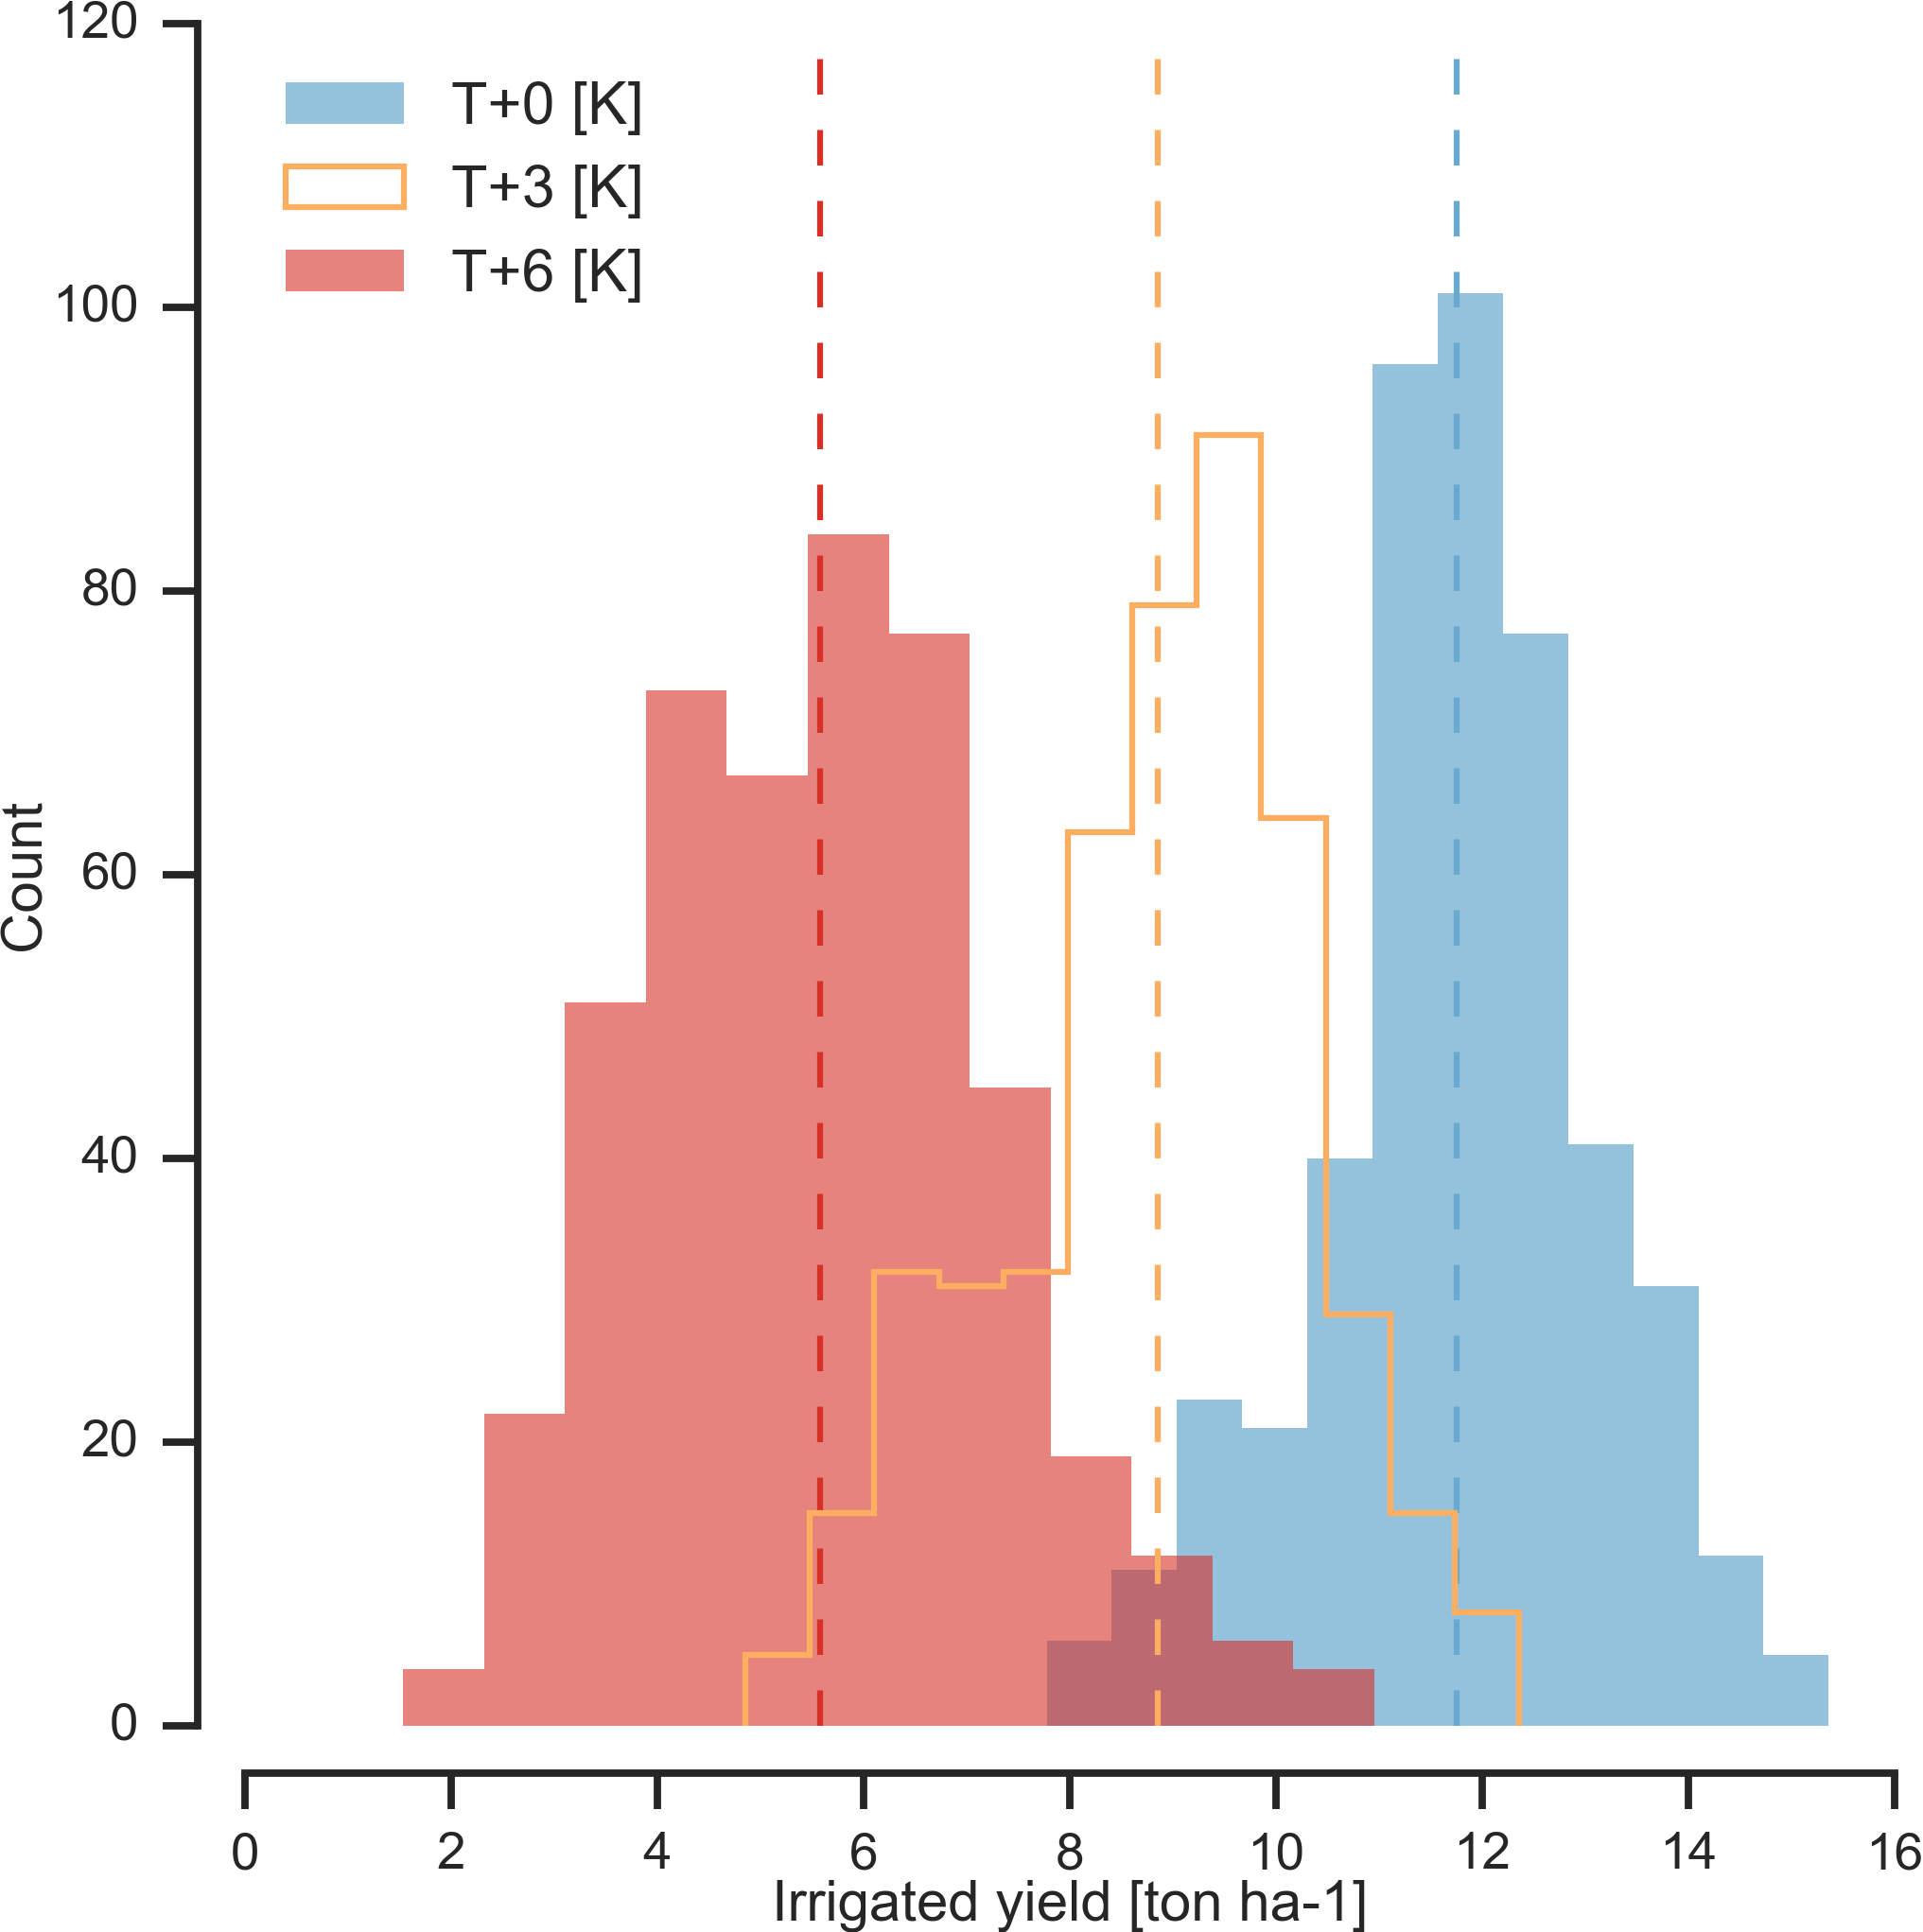
\includegraphics[width=8.3cm]{figures/hist_year.png}
   \caption{
   Example showing results of 
increased crop yield sensitivity to year-over-year climate variations 
under climate stress. Figure shows distributions of yields from examples 
of Figure 1, of irrigated (left) and rainfed (right) maize in Iowa in 
scenarios of altered temperature (left) and precipitation (right)..  
Under large warming (T+6) or drying (P-50\%), increased sensitivity means 
that distributions of year-over-year crop yields widen relative to 
present-day simulations, even though input timeseries has identical 
variance in climate drivers.

   Example showing climatological mean yields and distribution of yearly yields for three 30-year scenarios. 
   Figure shows irrigated maize for nine adjacent high-yield grid cells of Figure \ref{fig:yearvclim} from the pDSSAT model, for the baseline 1981-2010 historical climate (blue) and for scenarios with temperature shifted by T+3 (orange) and T+6 K (red), with other variables held at baseline values. 
   The stronger year-over-year temperature response with higher temperatures seen in Figure \ref{fig:yearvclim} is manifested here as larger variance in annual yields even though the variance in climate drivers is identical. 
   In this work we emulate not the year-over-year distributions but the climatological mean response (dashed vertical lines).
   }
   \label{fig:yearly}
\end{figure}

\begin{figure*}[ht]
\centering
    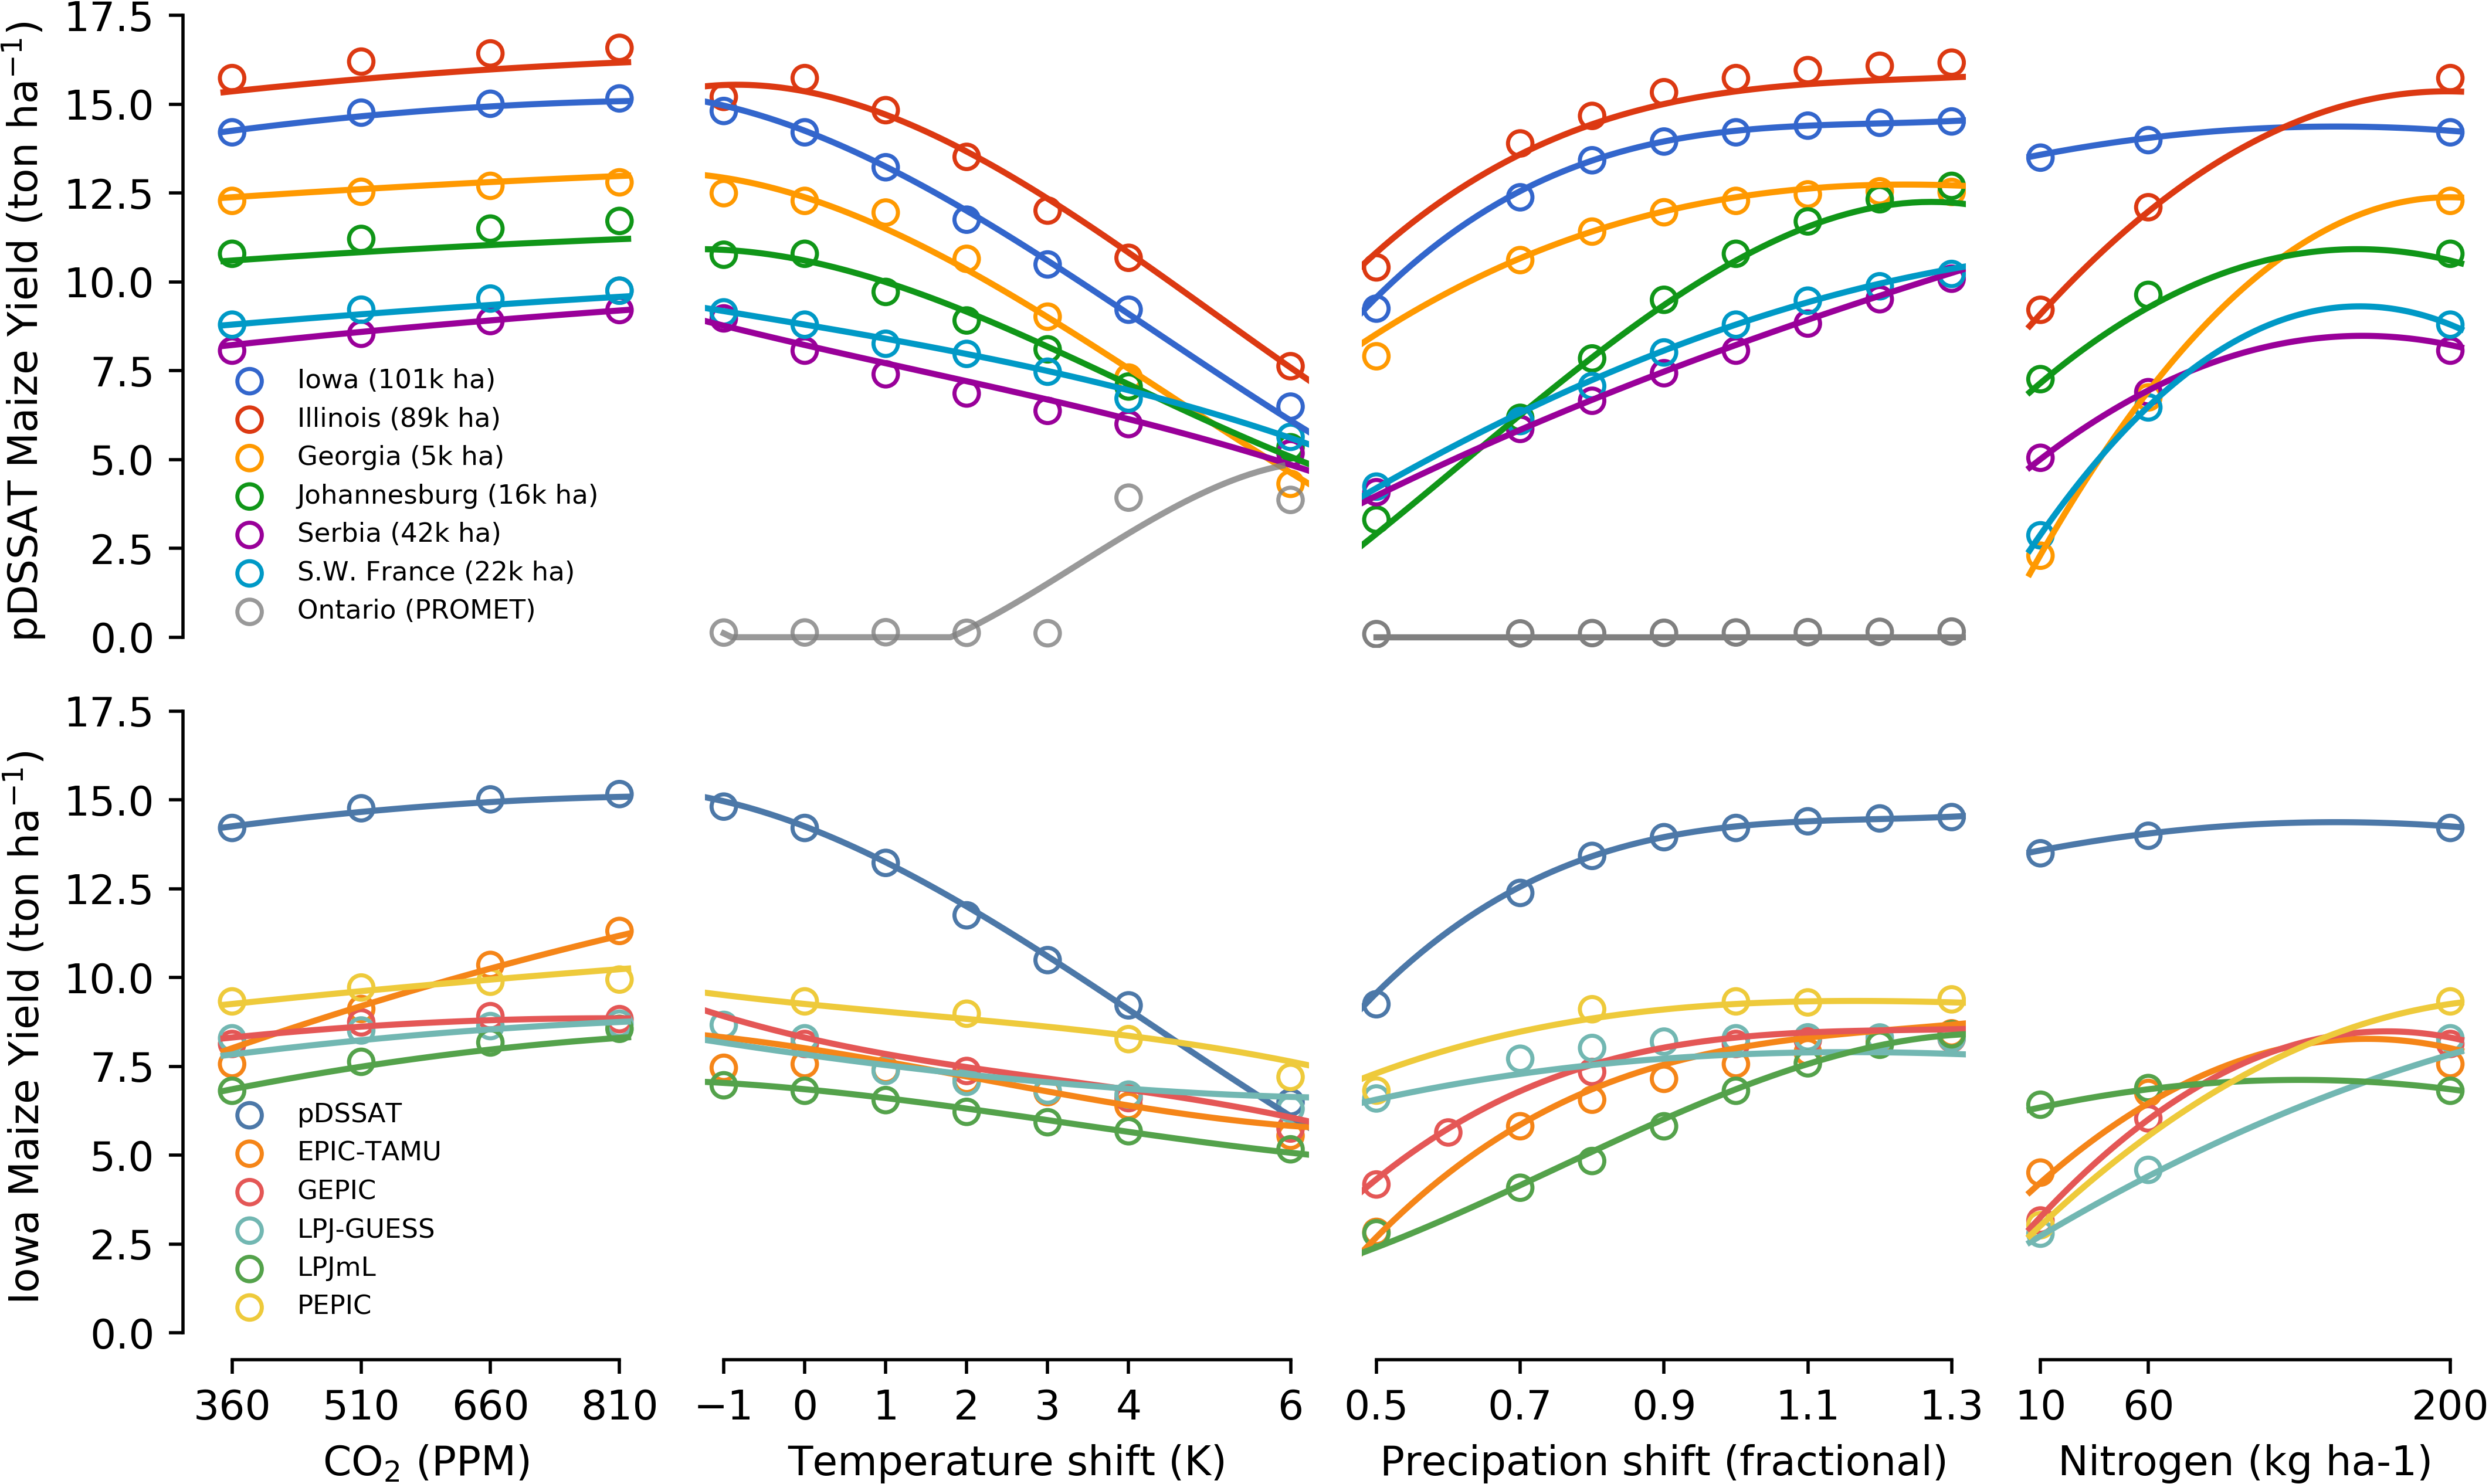
\includegraphics[width=16cm]{figures/regression_example.png}
    \caption{Illustration of spatial and across model variations in yield response successfully captured by the emulator. 
    Top row: simulations and emulations for rainfed maize in the pDSSAT model in six example locations selected to represent high-cultivation areas around the globe. 
    Legend includes hectares cultivated in each selected grid cell. 
    Bottom row: simulations and emulations from six models for rainfed maize in the same Iowa grid cell shown in the top row. 
    Models that do not simulate the nitrogen dimension are omitted for clarity.
    Each panel shows variation along a single variable, with others held at baseline values. 
    Dots show climatological mean yields and lines the results of the full 4D emulator of Equation \ref{eqn:features_original}. 
    In general the climatological response surface is sufficiently smooth that it can be represented within the sampled variable space by the simple polynomial used in this work. 
    While most model responses can readily emulated with a simple polynomial, some response surfaces diverge slightly from the polynomial approach (e.g.\ LPJ-GUESS here) and lead to emulation error, though error generally remains small relative to inter-model uncertainty. 
    The rainfed maize response in north-central Ontario is shown for the PROMET model as a good example of an area where the emulator fails.
    Note that some models are uncalibrated, increasing spread in absolute yields. 
    }
   \label{fig:regression}
\end{figure*}


Finally, we show a damage function constructed from the 4D emulation, aggregated to global yield, with simulated values shown for comparison (Figure \ref{fig:globe_em}, which shows maize on currently cultivated land; see Figures SXX-XX for other crops and dimensions). 
The emulated values closely match simulations even at this aggregation level.


\begin{figure}[ht]
    \centering
    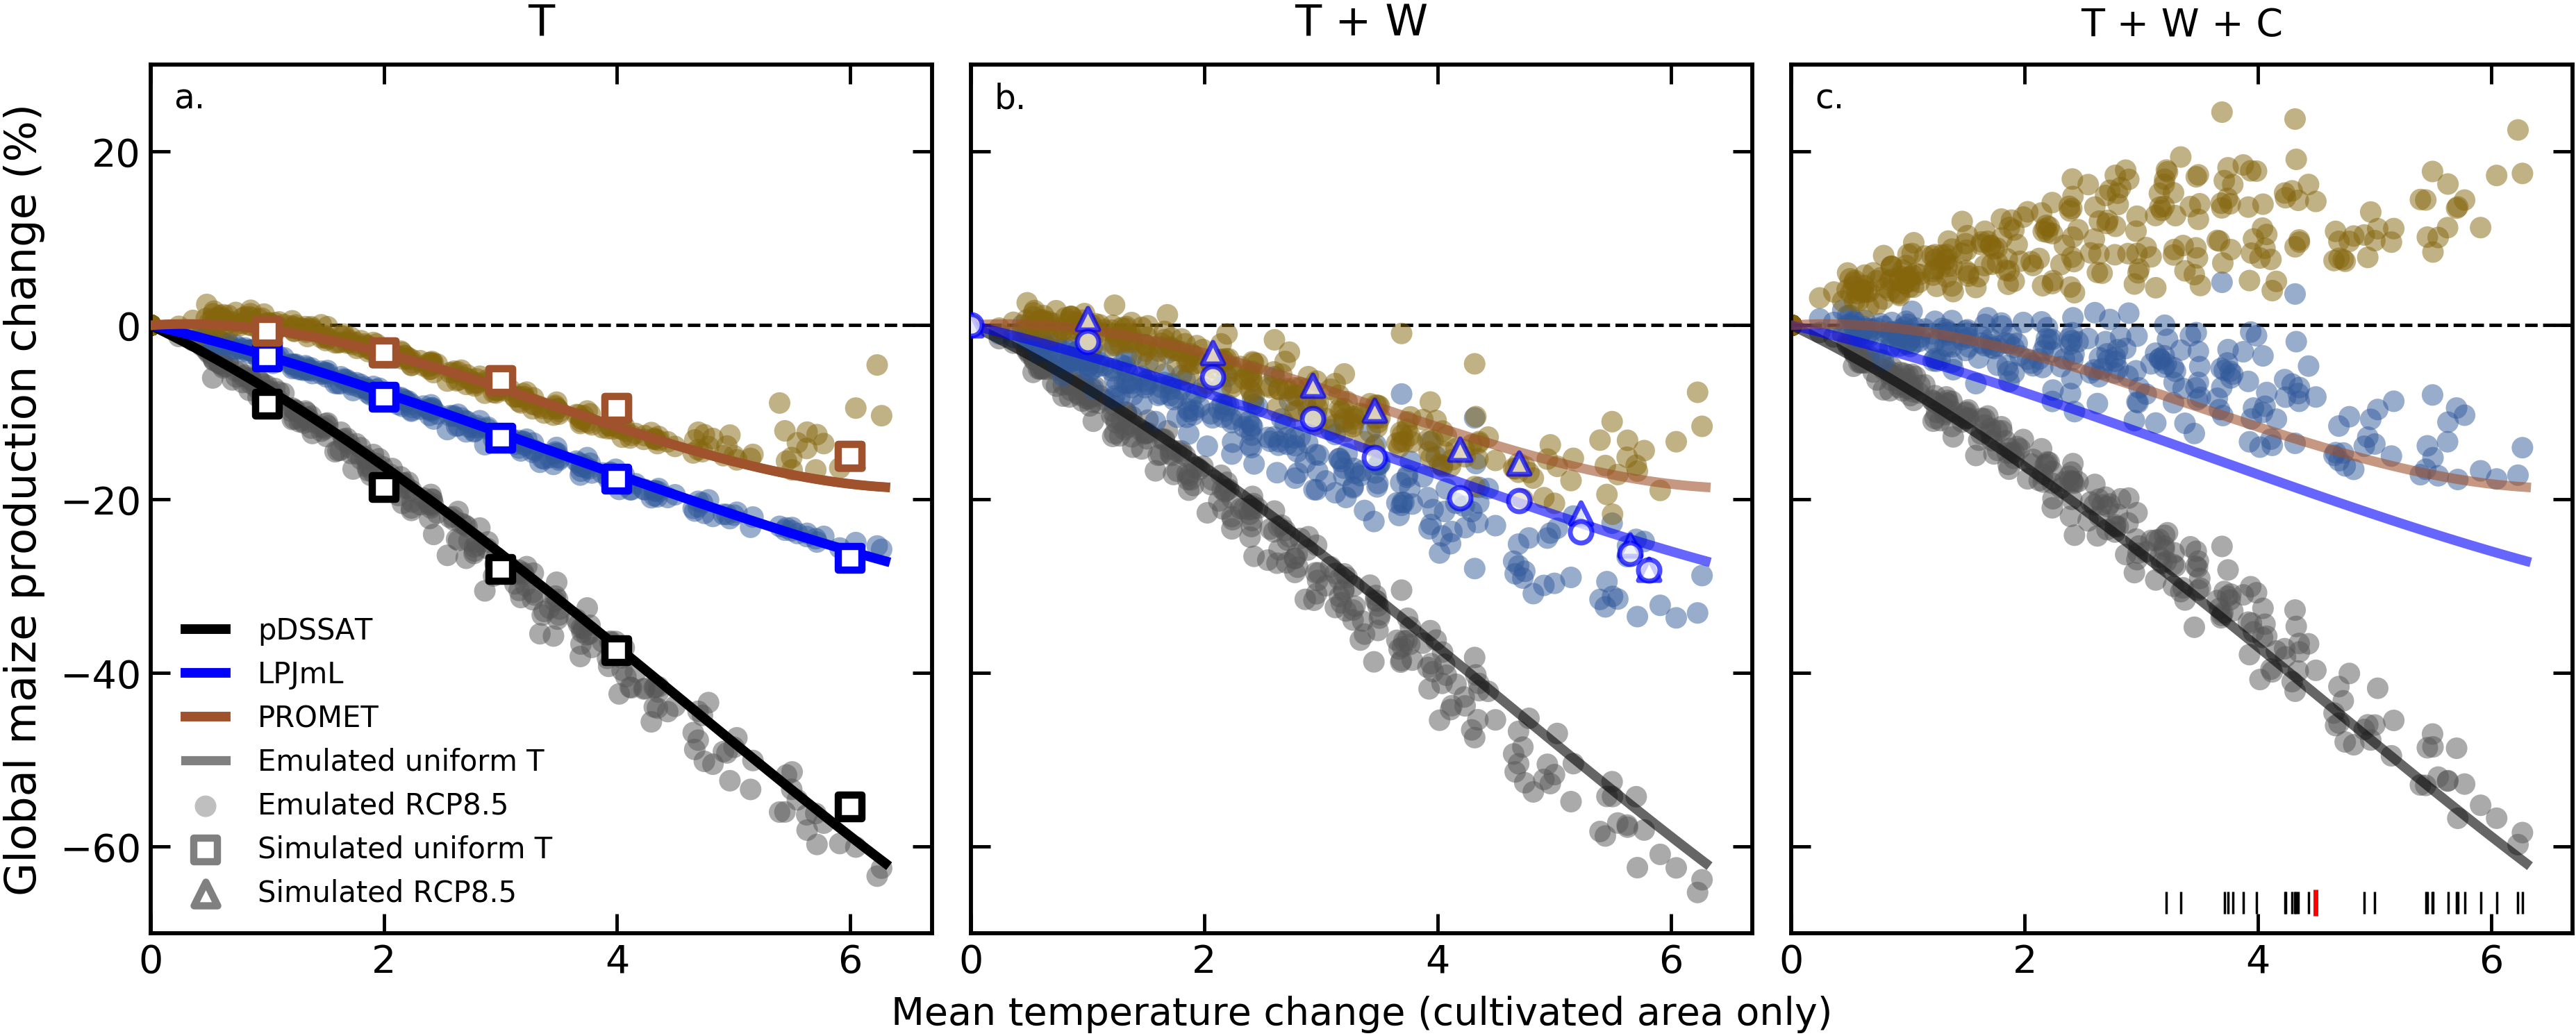
\includegraphics[width=8.3cm]{figures/global_em_maize.png}
    \caption{Global emulated damages for maize on currently cultivated lands for the GGCMI Phase II models emulated, for uniform temperature shifts with other inputs held at baseline. 
    (The damage function is created from aggregating up emulated values at the grid cell level, not from a regression of global mean yields.) 
    Lines are emulations for rainfed (solid) and irrigated (dashed) crops; for comparison, dots are the simulated values for the rainfed case.  
    For most models, irrigated crops show a sharper reduction than rainfed because of the locations of cultivated areas: irrigated crops tend to be grown in warmer areas where impacts are more severe for a given temperature shift (the exceptions are PROMET, JULES, and LPJmL, see \citet{Franke2019a} for more details). 
    For other crops and scenarios see Figures SXX-XX in the supplemental material.}
    \label{fig:globe_em}
\end{figure}
